\documentclass[12pt]{article}
\usepackage{float}
\usepackage{graphicx} 
\usepackage{mathtools}
\usepackage{amsmath, amsthm, amssymb}
\usepackage{siunitx} % SI Unit Functionality
\usepackage{times} % Times New Roman Font
\usepackage[symbols,americanvoltages]{circuitikz}%Circuit Illustration Package
\usepackage{steinmetz} %allows use of \phasor
\lefthyphenmin=5 %STOP HYPHENATING SMALL WORDS
\usepackage[toc,page]{appendix}

\title{\huge\bfseries Three Phase Open Loop Configuration PWM Generator for Use in Low Speed Brushless Motor Control
}
\author{
  \\
  \\
  \\
  \huge Santos, Matthew\\
  \\
  \texttt{\huge 103103503}
  \and
  \\
  \\
  \\
  \huge Schulz, Kurtis\\
  \\
  \texttt{\huge 104077177}
}
\date{\phantom\\
    \phantom\\
    \phantom\\
    \phantom\\
    \phantom\\
    \phantom\\
    {\scshape\Large University Of Windsor}\\
    \phantom\\
    {\Large\itshape Department of Computer and Electrical Engineering}\\
    \phantom\\
    \phantom\\
    \phantom\\
    \phantom\\
    Submitted April 3rd, 2016
}

\begin{document}

\begin{titlepage}
	\centering
	
\includegraphics[width=0.65\textwidth]{Data/UW_Header.png}\par\vspace{1cm}

	{\huge\bfseries Three Phase Open Loop Configuration PWM Generator for Use in Low Speed Brushless Motor Control\par}
	\vspace{1cm}
	{\scshape\Large 88-226-01: Electronics I\par}
	\vspace{1cm}
	{\scshape\Large Project Final Report \par}

	\vspace{2cm}
	{\Large\itshape Department of Computer and Electrical Engineering\par}
	\vfill
	Attention to\par
	Dr.~Mitra \textsc{Mirhassani}

	\vfill

% Bottom of the page
	{\large April 3rd,2016\par}
\end{titlepage} %done

\maketitle

\pagebreak
\tableofcontents
\pagebreak

\begin{abstract}
\addcontentsline{toc}{section}{Abstract}

    Brushless motors have both superior efficiency and durability however they require more complex control methods. Two of the more common control methods include sinusoidal pulse width modulation and trapezoidal pulse width modulation. This report seeks to design, build and evaluate a brushless motor control circuit that implements both of these techniques without the use of any positional feedback information.
    
    This circuit was realized through the coalescence of several smaller sub-circuits including that of a Wien Bridge Oscillator, Triangle Wave Generator, Three Phase Generator, Three Phase Comparator, a Modulation/Inversion Circuit, and an H-Bridge Driver. Physical analysis of the initial prototype revealed several imperfections arising from the non-idealities present in real world devices. These include instability in Wien Bridge Oscillations, deviations from expected phase shifts, and the presence of back-emf voltage waveforms generated through the rotating of the motor.
    
    In conclusion it was successfully shown that both SPWM and TPWM control techniques were capable of actuating the motor in frequency ranges between $5Hz$ to $95Hz$ while also allowing for the regulation of overall current delivered to the motor. Lastly it was observed that in accordance with expectations the method of SPWM control produced smoother actuation in contrast to the more bumpy TPWM technique.
    
\end{abstract}

\section{Introduction}%done

Electric motors serve as one of the most practical methods of transferring electrical energy into mechanical motion and have been in widespread use since its initial invention in 1827 by Hungarian physicist Anyos Jedik\cite{wiki:xxx}. Since then this mechanism has been refined and improved endlessly and now comes in a number of variations. Some of the most distinguished of which include the Brushed DC Motor, Brushless DC Motor (BLDC), AC Induction Motor, AC Synchronous Motor, and the AC Linear Motor.

In terms of operation, the brushed DC motor is considered to be the simplest and also serves as a good foundation for understanding the general principles of operation for an electric motor. Within a brushed DC motor, there are five essential parts the axle, the commutator, the armature, the field magnet, and the brushes themselves. These components can be seen in Figure \ref{DCMotor} which illustrates a simple two pole variant.

\begin{figure}[H]
\centering
\caption{Components of a Simple Brushed DC Motor\cite{dirjish_2012}}
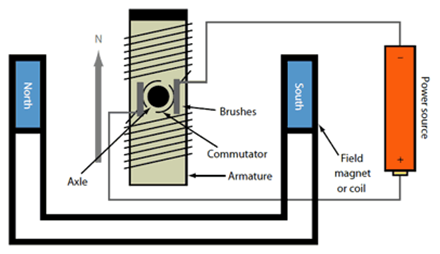
\includegraphics[scale=0.65]{Data/BrushMotor_Kurtis.png}
\label{DCMotor}
\end{figure}

As shown in the figure, the power source directly connects to the brushes which in turn interact with the commutator. The theory of operation is such that when the brushes induce a current flow across the commutator it generates an electromagnetic field due to the circular flow of current along the armature coils. This magnetic field then interacts with the field magnet and generates an magnetic force which acts to rotate the armature into a position that minimizes magnetic field intensity. However as the armature swings, the brushes which are held fixed slide across the commutator and upon the alignment of the two fields they reach a particular point and undergo the process of commutation or actuation. This process reverses the direction of current flow through the commutator and thus flips the magnetic field by $180^{\circ}$ which thus causes the magnetic force to be restored and rotation to continue.

While useful brushed motors do lack in efficiency and durability due to the mechanical interaction of the commutator and brushes which can induce electrical arching and degrade over time. In contrast however brushless motors allow for rotations without the need for any physical interaction with armature for commutation. Instead the task of controlling the direction of current is left to an external controller which senses the armature position and reverses current flow with appropriate calibrated timings. Typical brushless designs place the field magnet on the external rotor and the coils on the stationary internal stator however there is no set standard. An example of a three phase six pole brushless DC motor is illustrated in Figure \ref{BLDC}.

\begin{figure}[H]
\centering
\caption{Three-Phase Six-Pole Brushless Motor\cite{wilson_2012}}
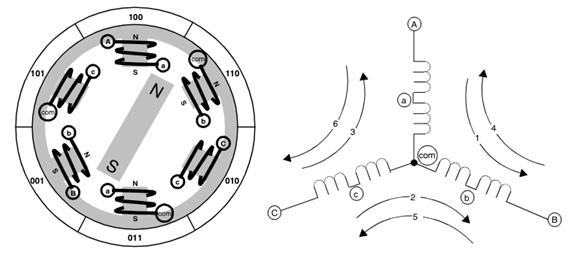
\includegraphics[scale=0.65]{Data/3PhaseMotor_Kurtis.png}
\label{BLDC}
\end{figure}

The addition of the third phase and extra poles allows for smoother operation and is another one of the more modern approaches to motor design. Poles are effectively connected together to make three main coil loops which alternate around the perimeter as shown in the figure. The external controller serves to cycle the current through each of these main loops in the sequence displayed in Table \ref{Control_Sequence} in order to active a rotational force.

\begin{table}[H]
\centering
\caption{Standard 6 Stage BLDC Commutation Sequence}
\label{Control_Sequence}
\begin{tabular}{|c|c|c|}
\hline
\textbf{Phase A}&\textbf{Phase B}&\textbf{Phase C}\\ \hline
$-V_{s}$&$+V_{s}$&$NC$\\ \hline
$NC$&$+V_{s}$& $-V_{s}$\\ \hline
$+V_{s}$&$NC$& $-V_{s}$\\ \hline
$+V_{s}$&$-V_{s}$& $NC$\\ \hline
$NC$&$-V_{s}$& $+V_{s}$\\ \hline
$-V_{s}$& $NC$& $+V_{s}$\\ \hline
\end{tabular}
\end{table}

Numerous current switching control methods exist for brushless motors however some current state of the art strategies include what is known as sinusoidal pulse width modulation (SPWM) and trapezoidal pulse width modulation (TPWM). These two methods are of particular interest and are discussed in detail in section~3 of this report.

Regardless of the control method, in order for the controller to identify the proper timing of when to perform commutation, a feedback signal from the motor is required which identifies the positioning of the rotor with respect to the stator. There are two primary means of feedback sensing. The first makes use of hall effect sensors to monitor the movement of the induced magnetic field around the motor. The positioning and calibration of these sensors is however of critical importance and thus they are typically built into high quality motors by default. For the more economical motors the second feedback method known as sensorless back-emf triggering is used. This method compromises the overall torque of the motor by allowing one of its main coils to remain idle during each sequence and serve instead as a sensor. As the motor rotates this coil receives an induced current through the rotation of the magnetic rotor about itself. Through the examination of the amplitude change in this induced current the moment of actuation can be directly observed and hence used for timing control. 

Both the hall effect sensors and back-emf techniques have been proven to work effectively at high actuation frequencies however issues arise with the back-emf method in the low frequency range. A slower rotation rate imposes a reduced rate of change in the magnetic field motion and thus corresponds to a very low amplitude back-emf. This in turn makes any actuation timing determination impossible. In order to compensate for this problem and allow the operation of brushless motors in the low frequency range without the need for hall effect sensors an open loop configuration is utilized.

Open loop configuration implies that their is no feedback signal and the controller just assumes the rotor position is traveling at the rate in which it is performing commutation. Utilizing this method low speed control becomes possible however as a compromise relative speed alterations must be kept small in order to give the motor enough time to acclimate to new speed setpoints. Although this restriction is not ideal, it is significantly more economical when compared with the cost of precision hall effect sensors.
\pagebreak
\section{Design Objectives}%done

Overall project design requirements include a restriction to the use of analogue devices for implementation along with the required use of at least one 555 Clock Timer. In addition the overall cost of all non-passive components and elements not included in the provided circuit kit are limited by a maximum budget of \$10. While adhering to these regulations the following project specific design objectives were pursued in accordance with the request of a third party.

\begin{enumerate}
\item Primary Objectives
    \begin{enumerate}
     \item Ability to Actuate an "EMAX Model 2213-935kV" BLDC Motor
     \item Dynamic Speed Control (priority being low speed)
     \item Variable Current Output
    \end{enumerate}
\item Secondary Objectives
    \begin{enumerate}
    \item Modular/Adaptable Overall Design to Allow for Easy Transfer to Other Applications
    \item Incorporate advanced control techniques to examine any improvements in operation
    \end{enumerate}
\end{enumerate}

\section{State of the Art}%done

Numerous modern day BLDC controllers exist and are readily available in the form of integrated circuits and programmable micro-controllers. The majority of these devices make use of digital logic devices for control, consequently purely analogue variants are a rarity. There exists two primary methods by which to produce the necessary PWM pulses needed to operate a motor using analogue devices.
\pagebreak
\subsection{Sinusoidal Pulse Width Modulation}%done

This method is the most popular and considered by many to be the standard BLDC control method. It functions through approximating a sine wave using width varying pulses of uniform amplitude. These pulses are then directly used to control the switches responsible for switching the flow of current in the device. The reason pulses are utilized instead of sine waveform is due to the fact that the switches in question are generally current limiting devices that are by design only capable of operating above a specified minimum voltage level. Through the pulse approximation of the sine waveform the switches are able to properly transition from on to off states in a more gradual fashion which allows for smoother overall operation.

In order to generate the SPWM control pulses using analogue techniques a simple comparator circuit is used to examine a given input sine waveform to a reference high frequency triangle waveform. The resulting output of the comparator is thus a pulse width modulated approximation of the input sine wave. This method of control pulse generation is illustrated in Figure \ref{SPWMSample}.

\begin{figure}[H]
\centering
\caption{Three Phase Sinusoidal PWM Generation\cite{developer}}
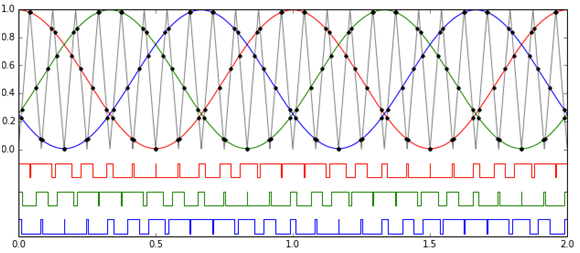
\includegraphics[scale=0.65]{Data/PWM_Waveform_Kurtis.png}
\label{SPWMSample}
\end{figure}

Naturally the relative accuracy of the approximation is relative to the frequency of the reference triangle waveform. For control device with a large operating frequency range it is sometimes necessary to also alter its reference waveform's frequency in parallel.
\pagebreak
\subsection{Trapezoidal Pulse Width Modulation}%done

Similar to the SPWM technique the TPWM method works by approximating a trapezoidal waveform using uniform amplitude pulses. The generation of these signals is carried out in exactly the same way as its sinusoidal counterpart and is illustrated in Figure \ref{TPWMSample} for a single phase.

\begin{figure}[H]
\centering
\caption{Trapezoidal PWM Generation\cite{Patel_useof}}
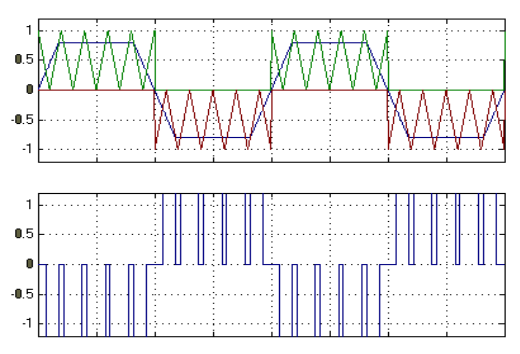
\includegraphics[scale=0.65]{Data/TPWMSample.png}
\\Note: Switches only trigger on positive pulses
\label{TPWMSample}
\end{figure}

As evident through the figure TPWM has a more steady driving force due to its plateau region which is sometimes more desirable depending on the motor specific application. In contrast however it has a much more abrupt transition from on to off states that consequently leads to more bumpy rotations then its SPWM counterpart. 

%(Kurtus is this you taking a shot at me???)
%There are many examples of motor controlling circuits online, but most of these circuits were quite simple to assemble, and nothing really would have been learned from submitting one of those designs as the final product. Instead of copying the designs straight from the Internet, it was decided that a custom design was going to be created and tested.


%This circuit is custom in a variety of ways. One of these ways is that instead of a simple DC motor being controlled, the motor used in this design is called a brushless DC electric motor (BLDC motor). The BLDC motor acts slightly different from the brushed DC motor because of the way that the rotation is generated.

\section{Deliverables}%done (improve?)

In order to satisfy the design objectives of the project and grant full control of the proposed "EMAX" motor at low speeds, the following deliverables were proposed.

\begin{enumerate}
\item Controlled Actuation Speeds ranging from <1Hz to 5Hz
\item Current Regulation from 0 to 1.5 Amps at any frequency
\item Ability to switch modes of operation for comparing control techniques
\begin{enumerate}
\item Incorporation of the SPWM Control Technique
\item Inclusion of a rough TPWM Control Technique
\end{enumerate}
\item Ability to be powered from any dual regulated voltage supply with reasonably wide input voltage operational limits.
\item Modular Design strategy to allow easy addition of additional functions after project submission (brakes, back-emf detection, reverse rotation, etc).
\item Calibration of the overall circuit to allow for full range control of the proposed "EMAX" motor in open loop configuration.
\end{enumerate}

\section{Design Methodology}%done

In order to accomplish the design task extensive research was conducted into existing designs. However none of the observed schematics fulfilled the both the requirement of using purely analogue devices and the requirement of remaining within the proposed budget without trivializing circuit construction through the use custom integrated circuits. Thus a fully custom overall circuit design was proposed that could perform both SPWM and a rough form of TPWM. This overall circuit design is summarized in Figure \ref{Circuit_Schematic_Summary} and illustrated in Appendix A.1 in full detail, the respective sections of this design and their functionality are individually described in the proceeding sections.

\begin{figure}[H]
\centering
\caption{Overall Circuit Design Block Diagram}
\includegraphics[scale=0.49]{Circuits/Overall_Design_Block.png}
\label{Circuit_Schematic_Summary}
\end{figure}

\subsection{Sine Wave Generation}%done

In order to accomplish full frequency control of sine waveform the use of a 555 timer was dismissed due to limitations in duty cycle control over large frequency ranges. Instead the more typical Wien Bridge Oscillator approach was selected and appropriately controlled through the use of a $10k\Omega$ POT resistor appropriately named $R_s$ for speed. The finalized design of the oscillator can be seen in Appendix~A.2.

The Wien Bridge oscillator works by establishing a feedback path through an operational amplifier with a set gain. The gain in this particular setup is established through resistors $R1$ and $R2$ and set to be precisely $A=3$ with hindsight. Along the feedback path are two impedances consisting of an RC series circuit and a RC parallel circuit in series which form a selective RC network. Treating them as a hypothetical voltage divider allows for the quick derivation of the associated transfer function. Further simplifying by setting the feedback resistors and capacitors equal produces the following relation.

\begin{equation}
    H_{feedback}(s)= \frac{RCs}{R^2C^2s^2+3RCs+1}
\end{equation}

Substituting in $s=j\omega$ and applying the op-amp gain $A_{o}$ to this equation results in the following relation for overall circuit gain.

\begin{equation}
    A(\omega)= \frac{A_oj\omega RC}{1+3j\omega RC-\omega^2R^2C^2}
\end{equation}

Now in order for the input and output waveforms to be in phase it is required that $1-\omega^2R^2C^2=0$ which implies that $\omega=1/RC$ and thus the selective frequency is determined to be as follows.

\begin{equation}
    f=\frac{1}{2\pi RC}
\end{equation}

Under this condition the gain equation simplifies to $A=A_o/3$ which implies that for an op-amp gain of less then 3 the output waveform will decay and only remains stable for $A_o=3$. For the case of $A_o>3$ the waveform grows in amplitude until it saturates as a result of the upper limits in which the op-amp can operate. 

In this circuit the diodes act to establish variations in op-amp gain in order to help maintain $A_o=3$. Finally the output of the oscillator is appropriately buffered at half magnitude to allow for some headroom in the upcoming stages. The results of LT-spice simulations on the proposed circuit are illustrated in Appendix B.1 and demonstrate the effectiveness of the control of frequency through alterations in $R_s$.

\subsection{Triangle Wave Generation}%done

The generation of the required high frequency triangle waveform was accomplished through the aggressive filtering of a high frequency 555 timer square wave signal as shown in Appendix A.3. In order to remove the 555 timer's intrinsic DC offset, it's reference to ground was purposely connected to the negative supply voltage line. 

The 555 timer was of course configured in astable operating mode and utilizing the indicated component values its output is established as follows.

\begin{equation}
    f=\frac{1.44}{2RC}\approx 1532Hz
\end{equation}
\begin{equation}
    DutyCycle=\frac{0.69RC}{1.38RC}\approx 0.5
\end{equation}

Afterwards a low pass RC filter was introduced in order to generate an reasonable approximation to a triangle waveform. This waveform was then connected to an non-inverting operational amplifier which was used to both buffer the sensitive signal and provide gain control through the variation of $R_a$. The results of LT-spice simulations concerning the variations of $R_a$ are described in detail in Appendix B.2.

\subsection{Phase Generation}%done

In order to generate the required PWM control signals the output of the sine wave generator circuit needed to be separated into three offset phases this is accomplished using the circuit seen in Appendix A.4 through the use of the left most column of operational amplifiers. The upper operational amplifier acts as a unity gain inverting buffer and outputs the first phase as an inverse of the input sine waveform and hence at $180^{\circ}$ relative phase shift. The lower amplifier is however fed a phase shifted version of the input sine waveform as a result of an RC filter.

\begin{equation}
    \psi=-arctan(2\pi fRC)
\end{equation}

The values for R and C are carefully selected to maintain a $60^{\circ}$ shift at the provided input frequency. The use of a passive RC shifter in this section does reduce the signal amplitude reaching the lower op-amp and hence it is given a higher gain to compensate. The lower op-amp is also configured in non-inverting configuration thus establishing an output that is at $60^{\circ}$ with respect to the input waveform. Lastly the middle op-amp acts as a inverting summer of the two other phases. As such its output phase with respect to the input is $ (180^{\circ}+60^{\circ})+180^{\circ}=420^{\circ}$. Ignoring the reference to the input waveform it is clear that the relative phase shifts between these outputs are all offset by $120^{\circ}$ as desired. In order to verify the correct generation of all three phases an LT-spice simulation was conducted and the results as shown in Appendix B.3 showed perfect agreement.

In order to allow for full variation of the input frequency while maintaining the required phase shift value it was decided to have one control vary both accordingly. In order to accomplish this equations (3) and (5) were equated for frequency and the resulting capacitance values selected such that both the wien bridge resistor and the phase shift resistor would share the same value and could thus be controlled through a ganged potentiometer.

\subsection{Pulse Generation}%done

In the second half of the circuit illustrated in Appendix C.3 lives the core element of the controller design. Three op-amps are arranged in difference amplifier configurations with unity gains and serve to produce pulse signals by direct comparison of the three input sine wave phases to a reference signal. A two pole switch is utilized to control the reference waveform. Here SPWM pulses as mentioned in section 3.1 are generated by connecting the triangle wave generator to the reference input terminal and the initial stage of rough TPWM generation is produced through referencing to a negative DC voltage. LT-spice simulation results for the proposed configurations are illustrated in Appendix B.4 and B.5 respectively.

\subsection{Modulation and Inversion}%done

The circuit of Appendix A.5 is used to perform amplitude like modulation on the TPWM generated signals from the previous stage and perform unity gain inversion of the SPWM signals. For the case of the SPWM inversion this circuit has no effect as a relative phase shift of 180 degrees does not influence the overall result. Appendix B.7 illustrates the inversion portion of the circuit and its negligible effect. Instead the inversion is simply an accepted consequence of the need for operational amplifiers in inverting configuration for the TPWM mode of operation.

In the TPWM setting the input waveforms to this stage are the inverted versions of the desired PWM signals and as such need to be flipped. At the same time a trapezoidal like modulation is applied to the waveform by summing the triangle wave signal with the input wave using summing amplifiers in inverting configuration. The resulting output of this is shown in Appendix B.6. While not a true form of Trapezoidal Pulse Width Modulation it does serve to produce a magnitude controllable consistent strength PWM signal with sudden transitions in accordance with what TPWM signals are defined by.

\subsection{Power Generation and Distribution}%done

While the control pulses generated in the previous section could be used to drive a motor they lack the required current needed to produce enough torque. In order to achieve the needed current a system of power transistors is utilized and controlled through the PWM signals. For this circuit bipolar junction transistors were selected. The usual power transistor motor configuration circuit is known as an H-Bridge and is illustrated in Appendix A.6. It operates by switching the direction of current flow through each coil as shown in Figure \ref{HBridge}.

\begin{figure}[H]
\centering
\caption{Basic H-Bridge Operation}
\includegraphics[scale=0.62]{Data/H-BridgeOperation.png}
\label{HBridge}
\end{figure}

For this circuit the transistors act as switches and were operated near the middle of the saturation region. This was done intentionally so that regardless any potential timing irregularities the maximum amount of current traversing a node would not exceed 2A even in the event of a direct short. If needed however the transistors could easily be allowed to permit increased current flow by increasing the supply voltage level of $V_{cc}$.
\pagebreak
\section{Values and Constraints}%done

Utilizing the design strategy as outlined in the previous section three essential control parameters are needed to fully govern motor movement in addition to one operating mode switch. These controls and their respective functions are described below.

\begin{enumerate}
\item Variable Speed Control ($R_s$)
    \begin{itemize}
     \item A three gang $10k\Omega$ Potentiometer 
     \item Adjusts the Wien Bridge Oscilating Frequency
     \item Maintains the required $60^{\circ}$ phase shift in three phase generator
    \end{itemize}
\item Variable Current Control ($R_a$)
    \begin{itemize}
    \item A center tapped $5k\Omega$ Potentiometer
    \item Controls the effective magnitude of the triangle waveform and hence overall magnitude of the output PWM pulses
    \end{itemize}
\item Pulse Delay Control ($R_d$)
    \begin{itemize}
    \item A small $1k\Omega$ Trimming Potentiometer
    \item Used to control the time delay between pulse signals in TPWM operating mode
    \item Serves to prevent the simultaneous activation of H-bridge transistor vertical pairings
    \end{itemize}
\item Operating Mode Switch ($S_1$)
    \begin{itemize}
    \item Acts to switch between SPWM and TPWM operating modes
    \end{itemize}
\end{enumerate}

These control components as well as all other devices necessary for circuit implementation are illustrated in Table \ref{budget} alongside their respective costs.

\begin{figure}[H]
\centering
\caption{Parts List and Respective Cost Breakdown}
\includegraphics[scale=0.65]{Data/Final_Budget.png}
\label{budget}
\end{figure}

From the table it is clear that the overall budget was maintained in accordance with project requirements. It is additionally noted that the respective power supply and "EMAX" motor were provided on loan from the prospective customer in order to verify and test correct circuit operation and as such are not included in cost projections.%It is unfortunate that the proposed budget limit of $\$10$ existed as it prevented the development of a sensorless back-emf configuration.

\section{Physical Implementation}%done

Physical realization of the proposed circuit was conducted upon a standard prototype board and the various features of each sub-circuit evaluated at the time of its initial creation. The initial design and testing environment is illustrated in Figure~\ref{Setup} and demonstrates the availability of parts and testing apparatus.

\begin{figure}[H]
\centering
\caption{Circuit Construction Environment}
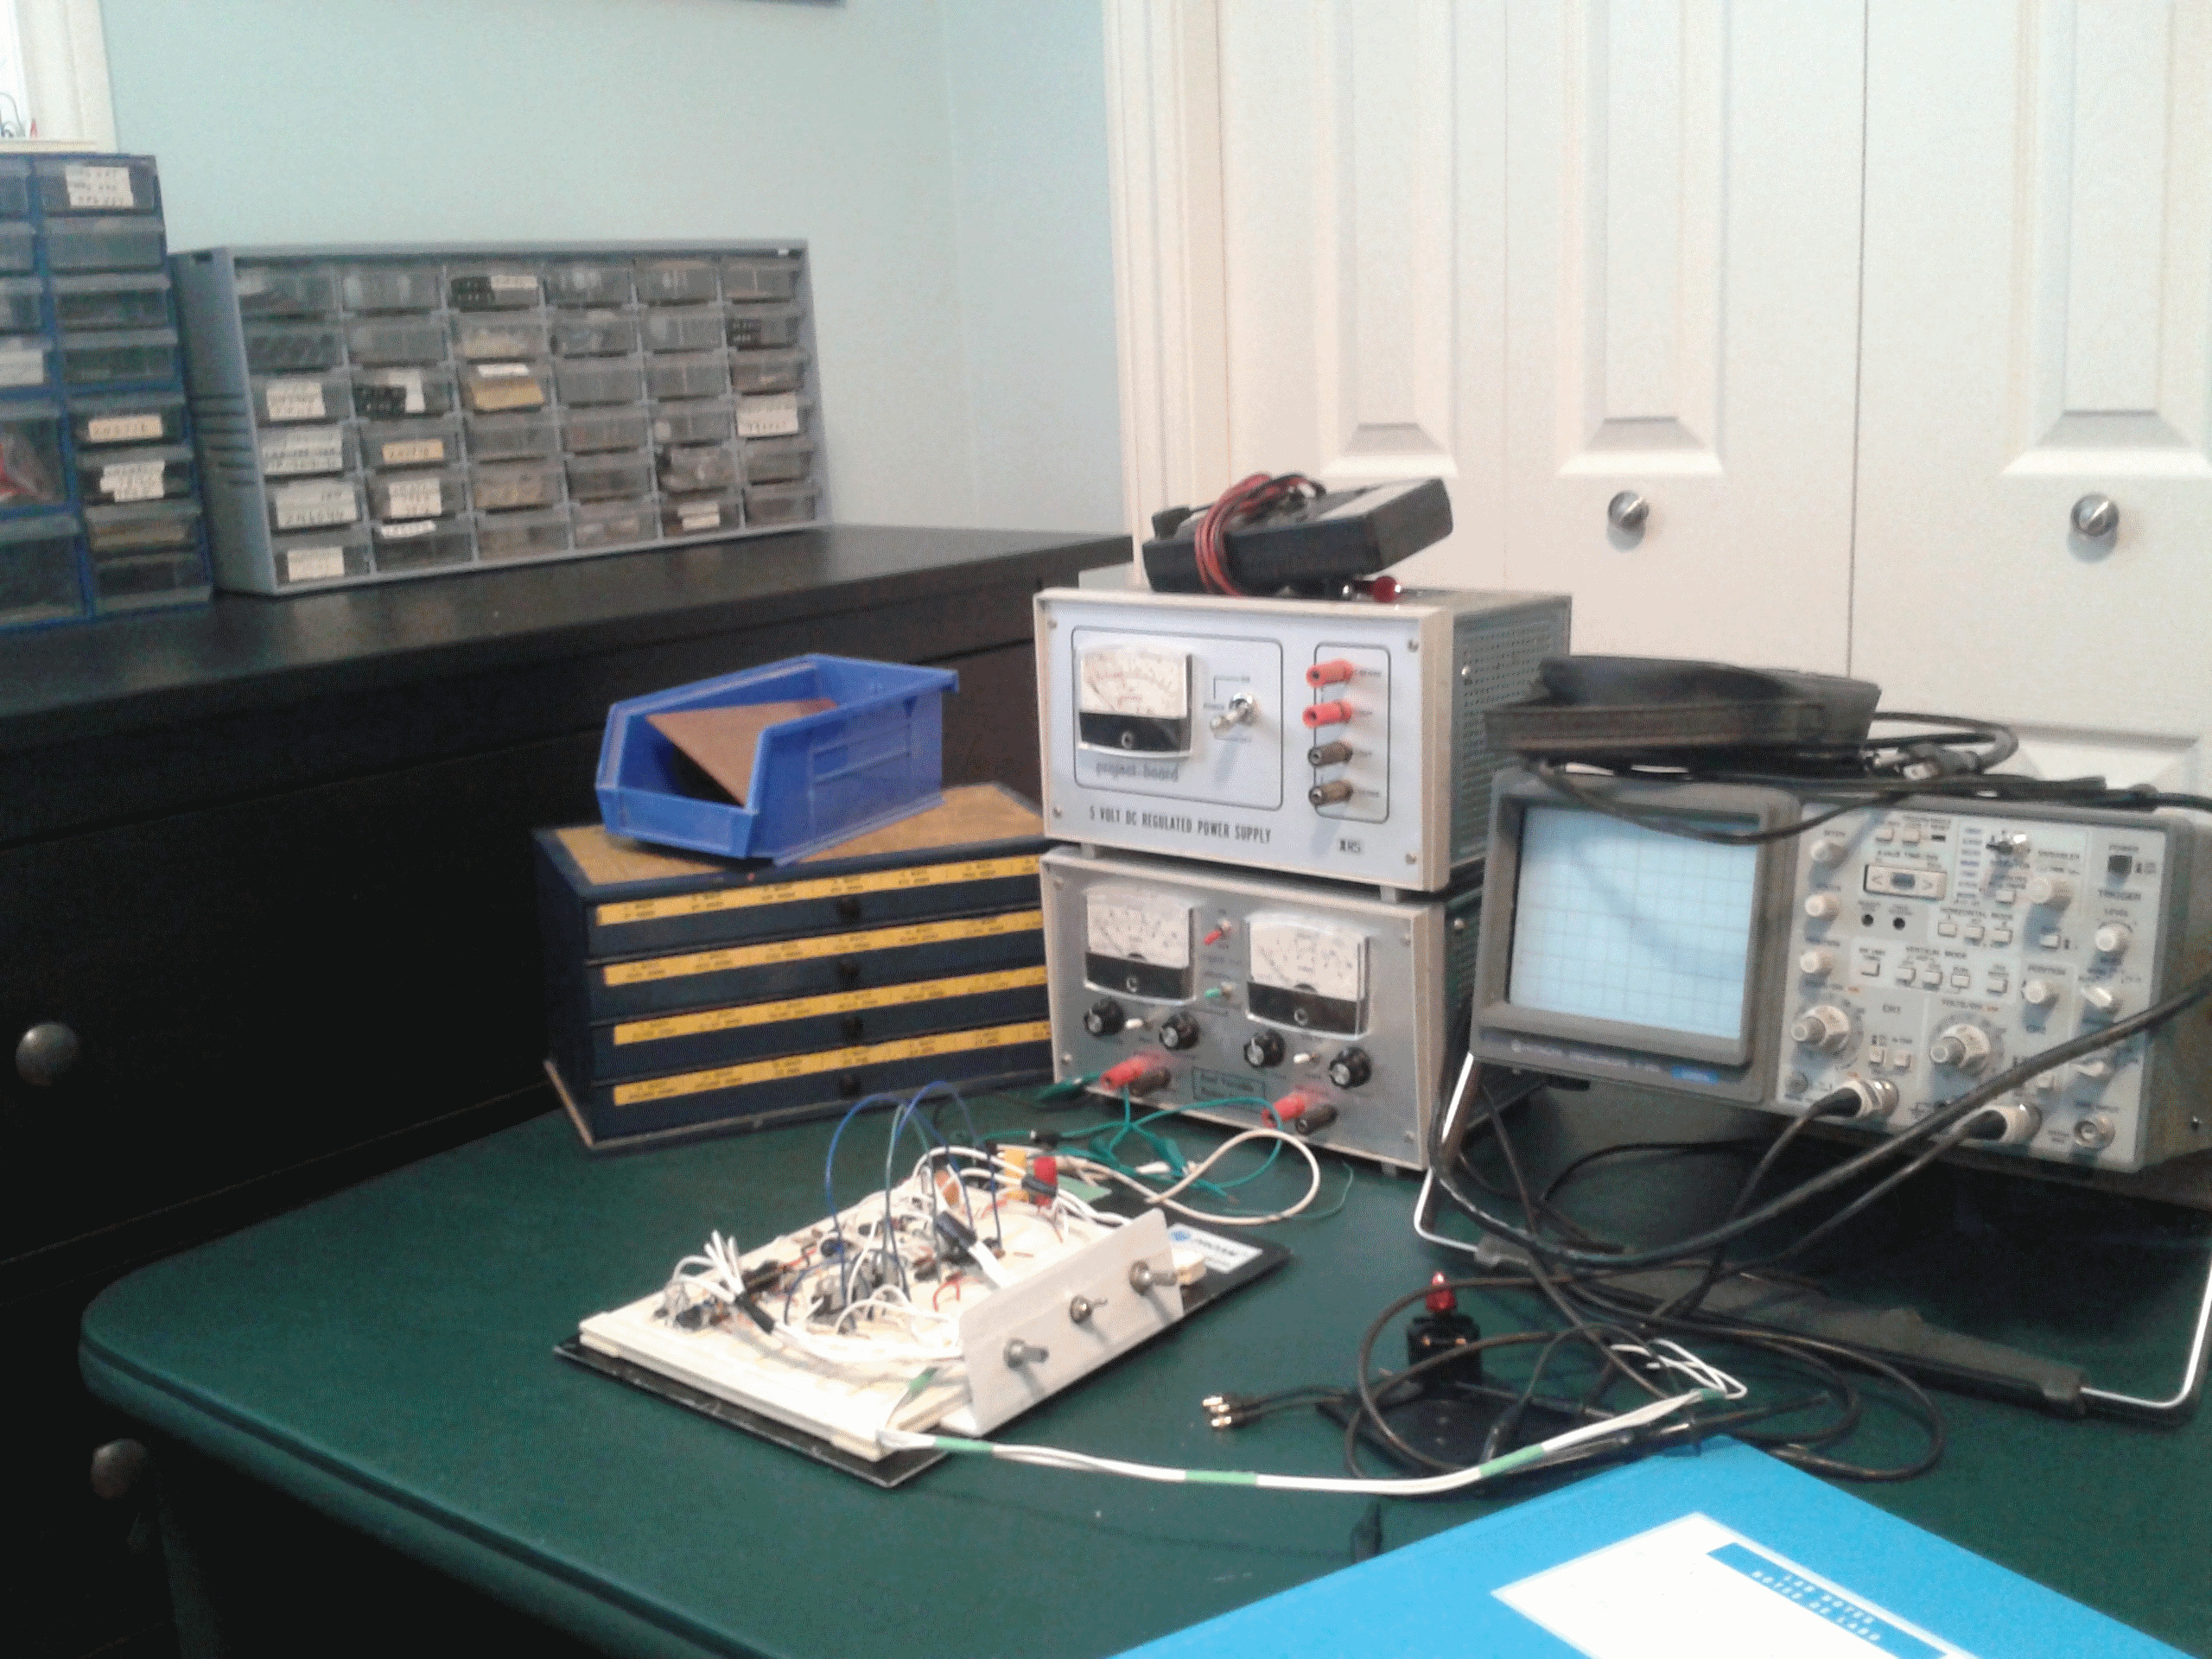
\includegraphics[scale=0.1]{Circuits/Setup.jpg}
\label{Setup}
\end{figure}

Over the course of construction several alterations to the proposed design were required in order to account for real world circuit behavior that was not observed in the simulations.

The first alteration was for the Wien Bridge Oscillator, the proposed design produced highly unstable waveforms as the relative gain across the op-amp fluctuated wildly. In order to rectify this the circuit design was altered to include a small trimming potentiometer to function as gain control. This resistor was placed in series with $R1$ and $R2$ and the diodes $D1$ and $D2$ were connected in parallel with it. The modified circuit is illustrated in Figure \ref{WBOFIXED} and was shown to provide superior operation. 

\begin{figure}[H]
\centering
\caption{Modified Wien Bridge Oscillator Schematic}
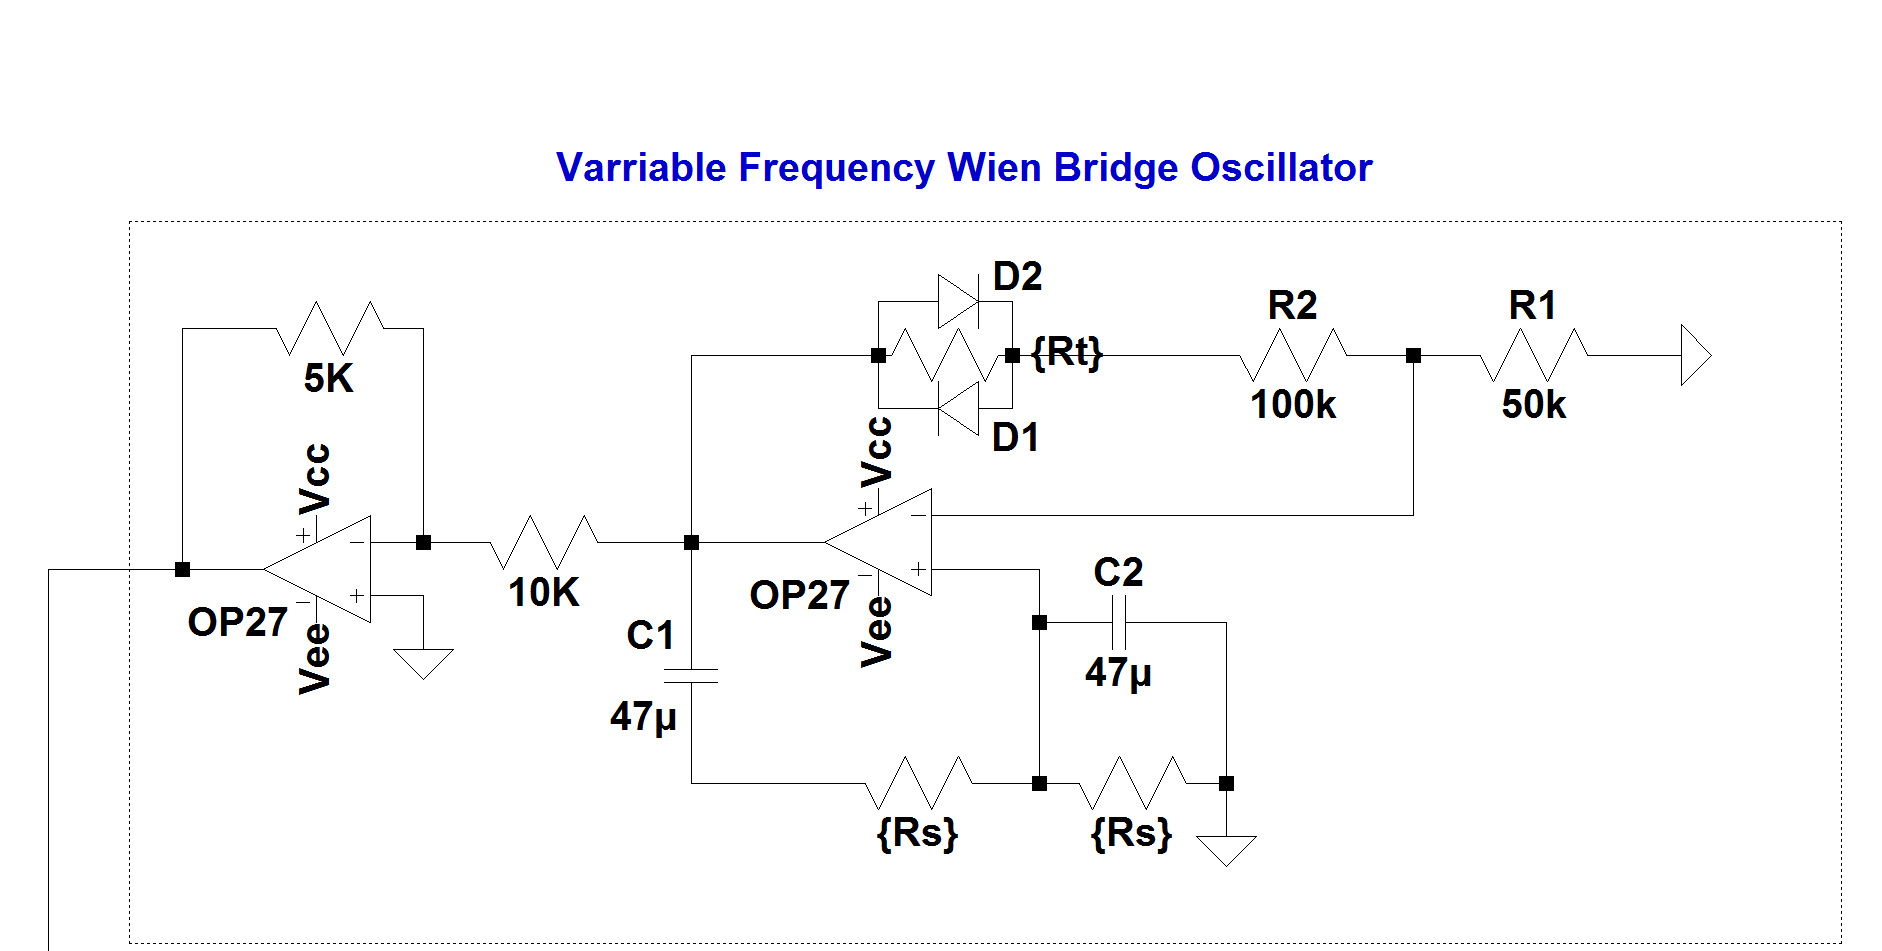
\includegraphics[scale=0.3]{Circuits/WBOFIXED.png}
\label{WBOFIXED}
\end{figure}

In addition upon observation of the physical operation of the motor it was shown that an actuation speed of $5Hz$ was to slow and could hardly be observed. To allow for the a better range of operation, the wien bridge capacitors $C1$ and $C2$ were swapped for $4.7\mu F$ versions which brought the upper range of frequencies to the $100Hz$ region. It is noted that speeds greater then $100Hz$ were tested and shown to be to fast and simply resulted in the motor slipping due to its own inertia which is one of the expected drawbacks to open loop configurations. The completed prototype is illustrated in Figure \ref{CircuitFinal} from a top down view.

\begin{figure}[H]
\centering
\caption{Finalized Prototype}
\includegraphics[scale=0.15]{Data/CircuitFinal.jpg}
\label{CircuitFinal}
\end{figure}


\pagebreak
\section{Experimental Results}%done

Following the successful completion of the physical prototype, the circuit was rigorously examined for performance and accuracy. The results of this analysis are presented in the following sections.

\subsection{Wien Bridge Oscillator}%done

First the operation of wien bridge oscillator was examined in order to verify that it produced the stable sine waveforms at various frequencies. Through direct observation it was seen that waveform stability existed throughout the low frequency range of operation but frequencies greater then $95Hz$ caused a complete collapse. This is theorised to be a result of the limiting tolerance of the utilized POT resistor $R_s$ as it is quoted to have deviations of up to $10\%$ and as such cannot operate effectively at extremely low values (it just becomes a short). 

To further verify the correct operation of the oscillator the variation of $R_s$ was examined in tandem with output waveform frequency and amplitude response. The results of this analysis are illustrated in Figures~\ref{WBOFrequency}~and~\ref{WBOAmplitude} respectively.

\begin{figure}[H]
\centering
\caption{Wien Bridge Oscillator Frequency Response}
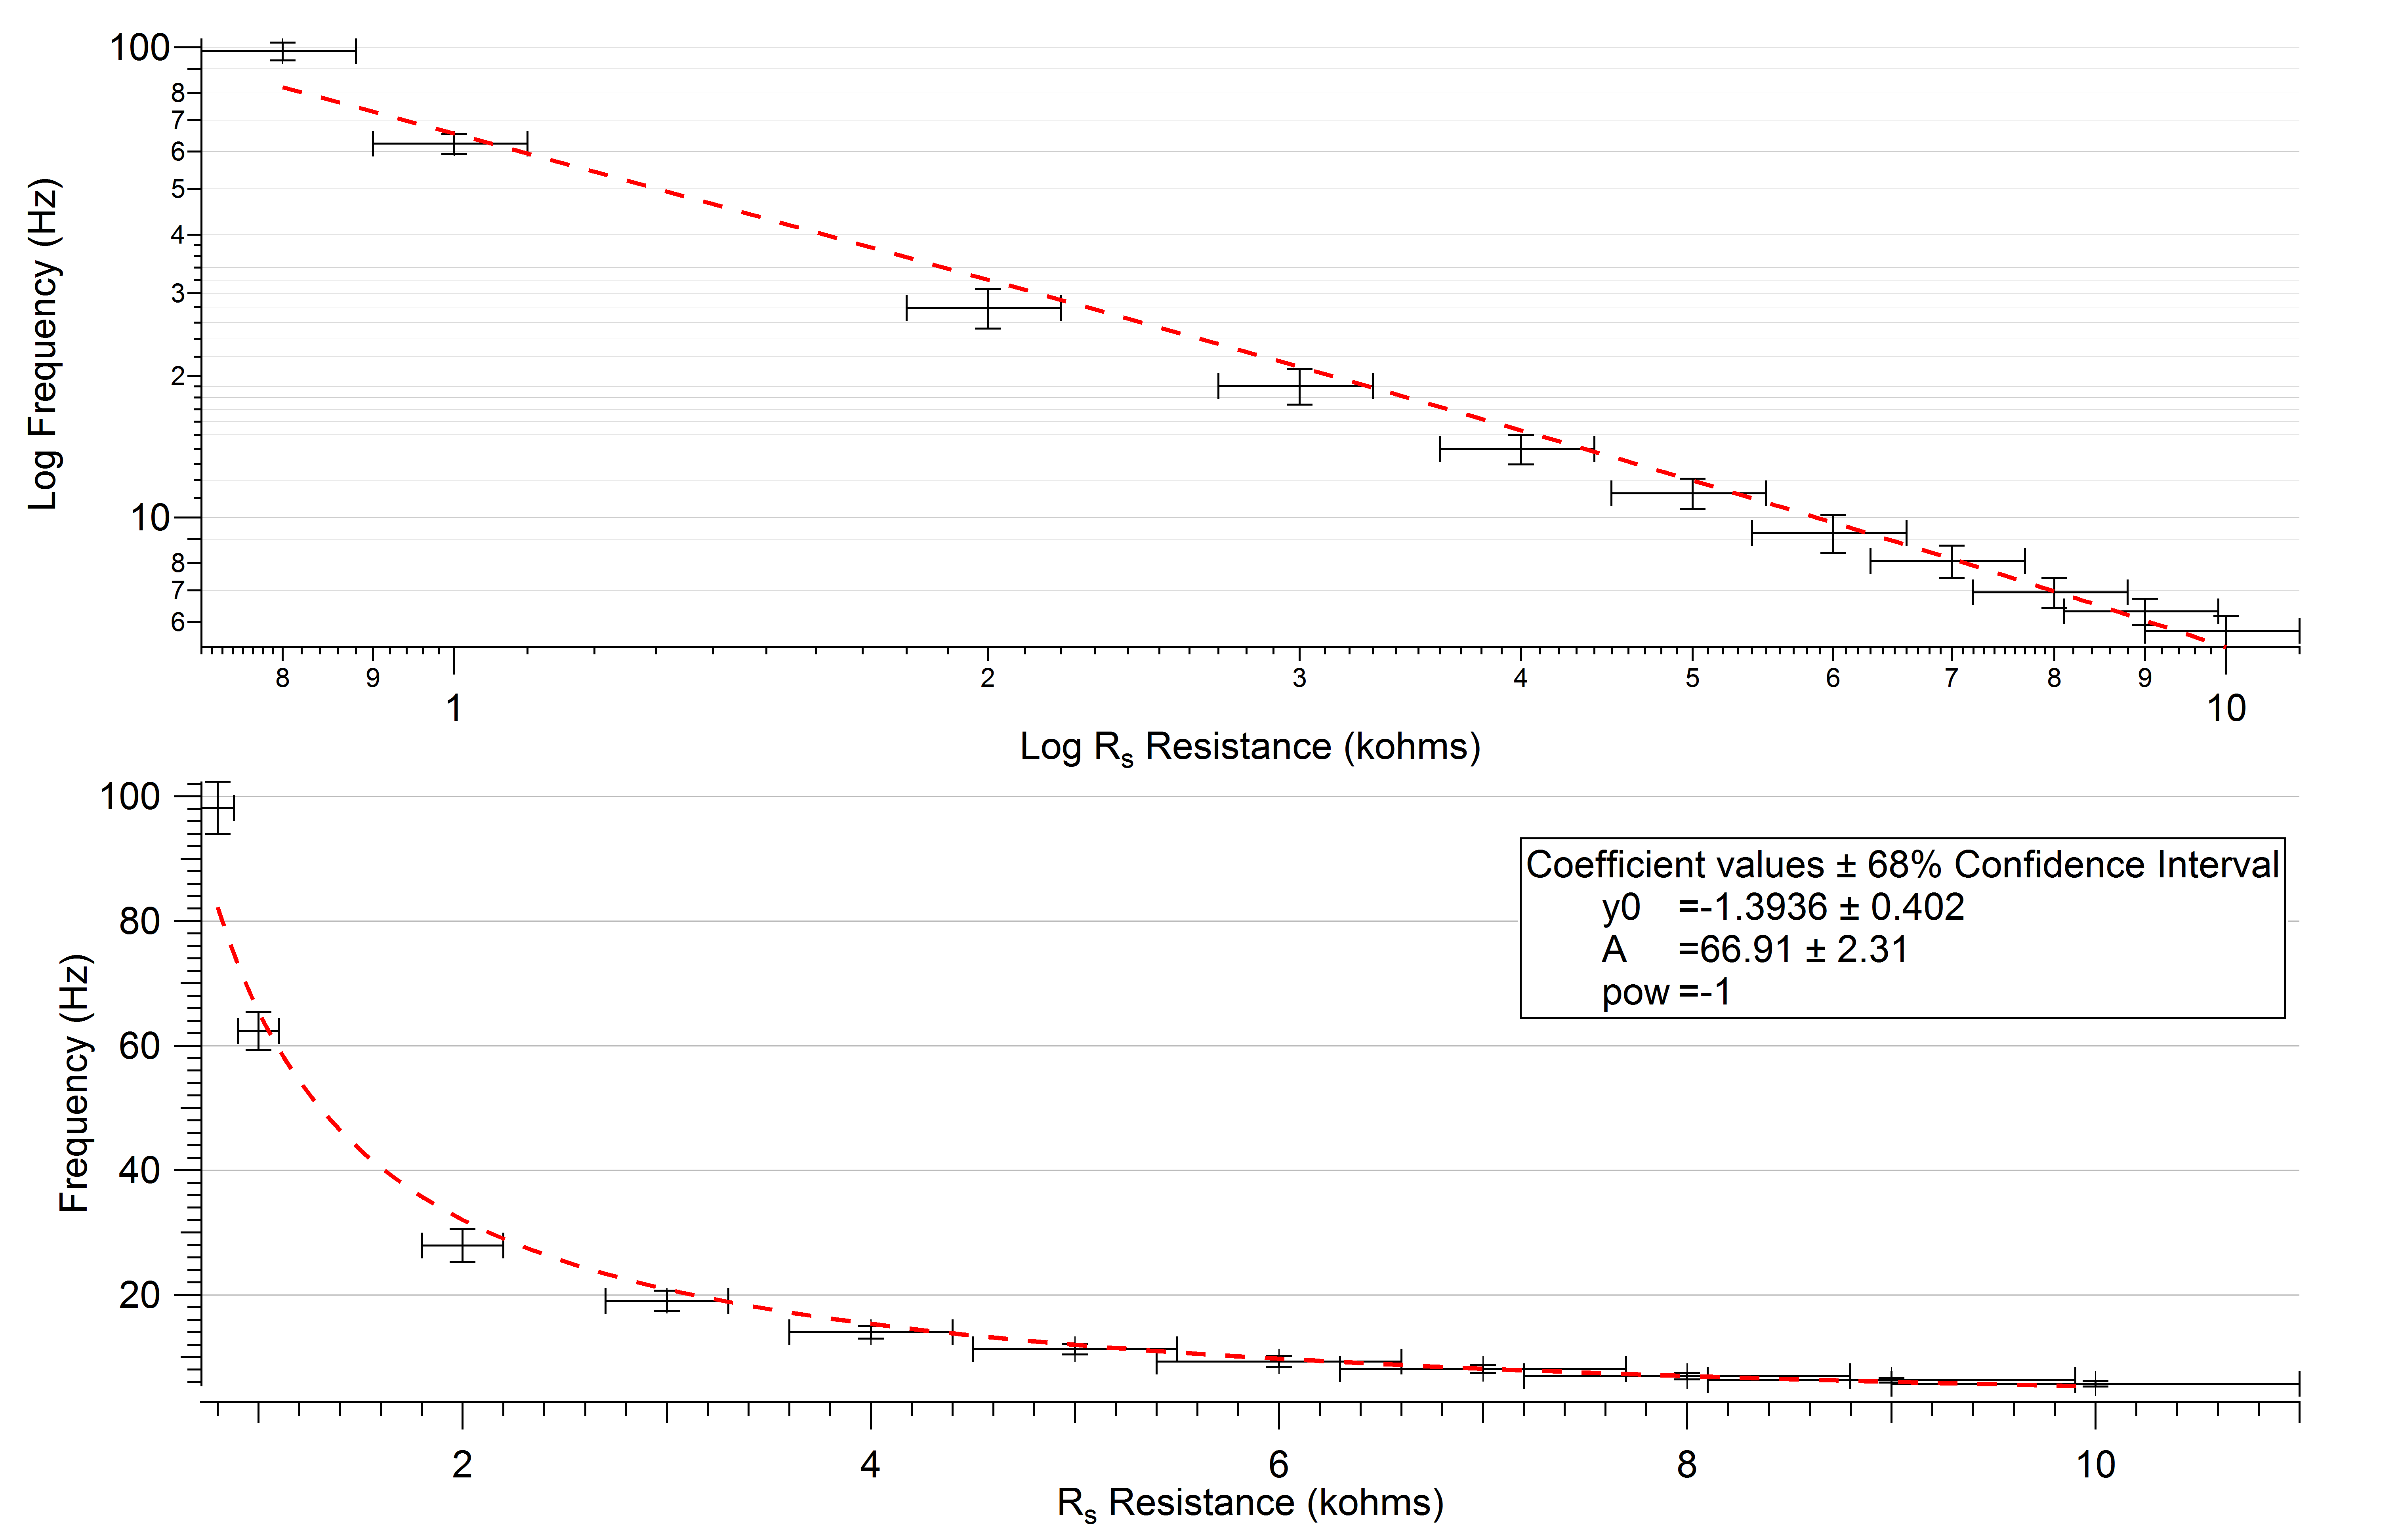
\includegraphics[scale=0.3]{Data/WienBridgeFrequency.png}
\label{WBOFrequency}
\end{figure}

\begin{figure}[H]
\centering
\caption{Wien Bridge Oscillator Amplitude Response}
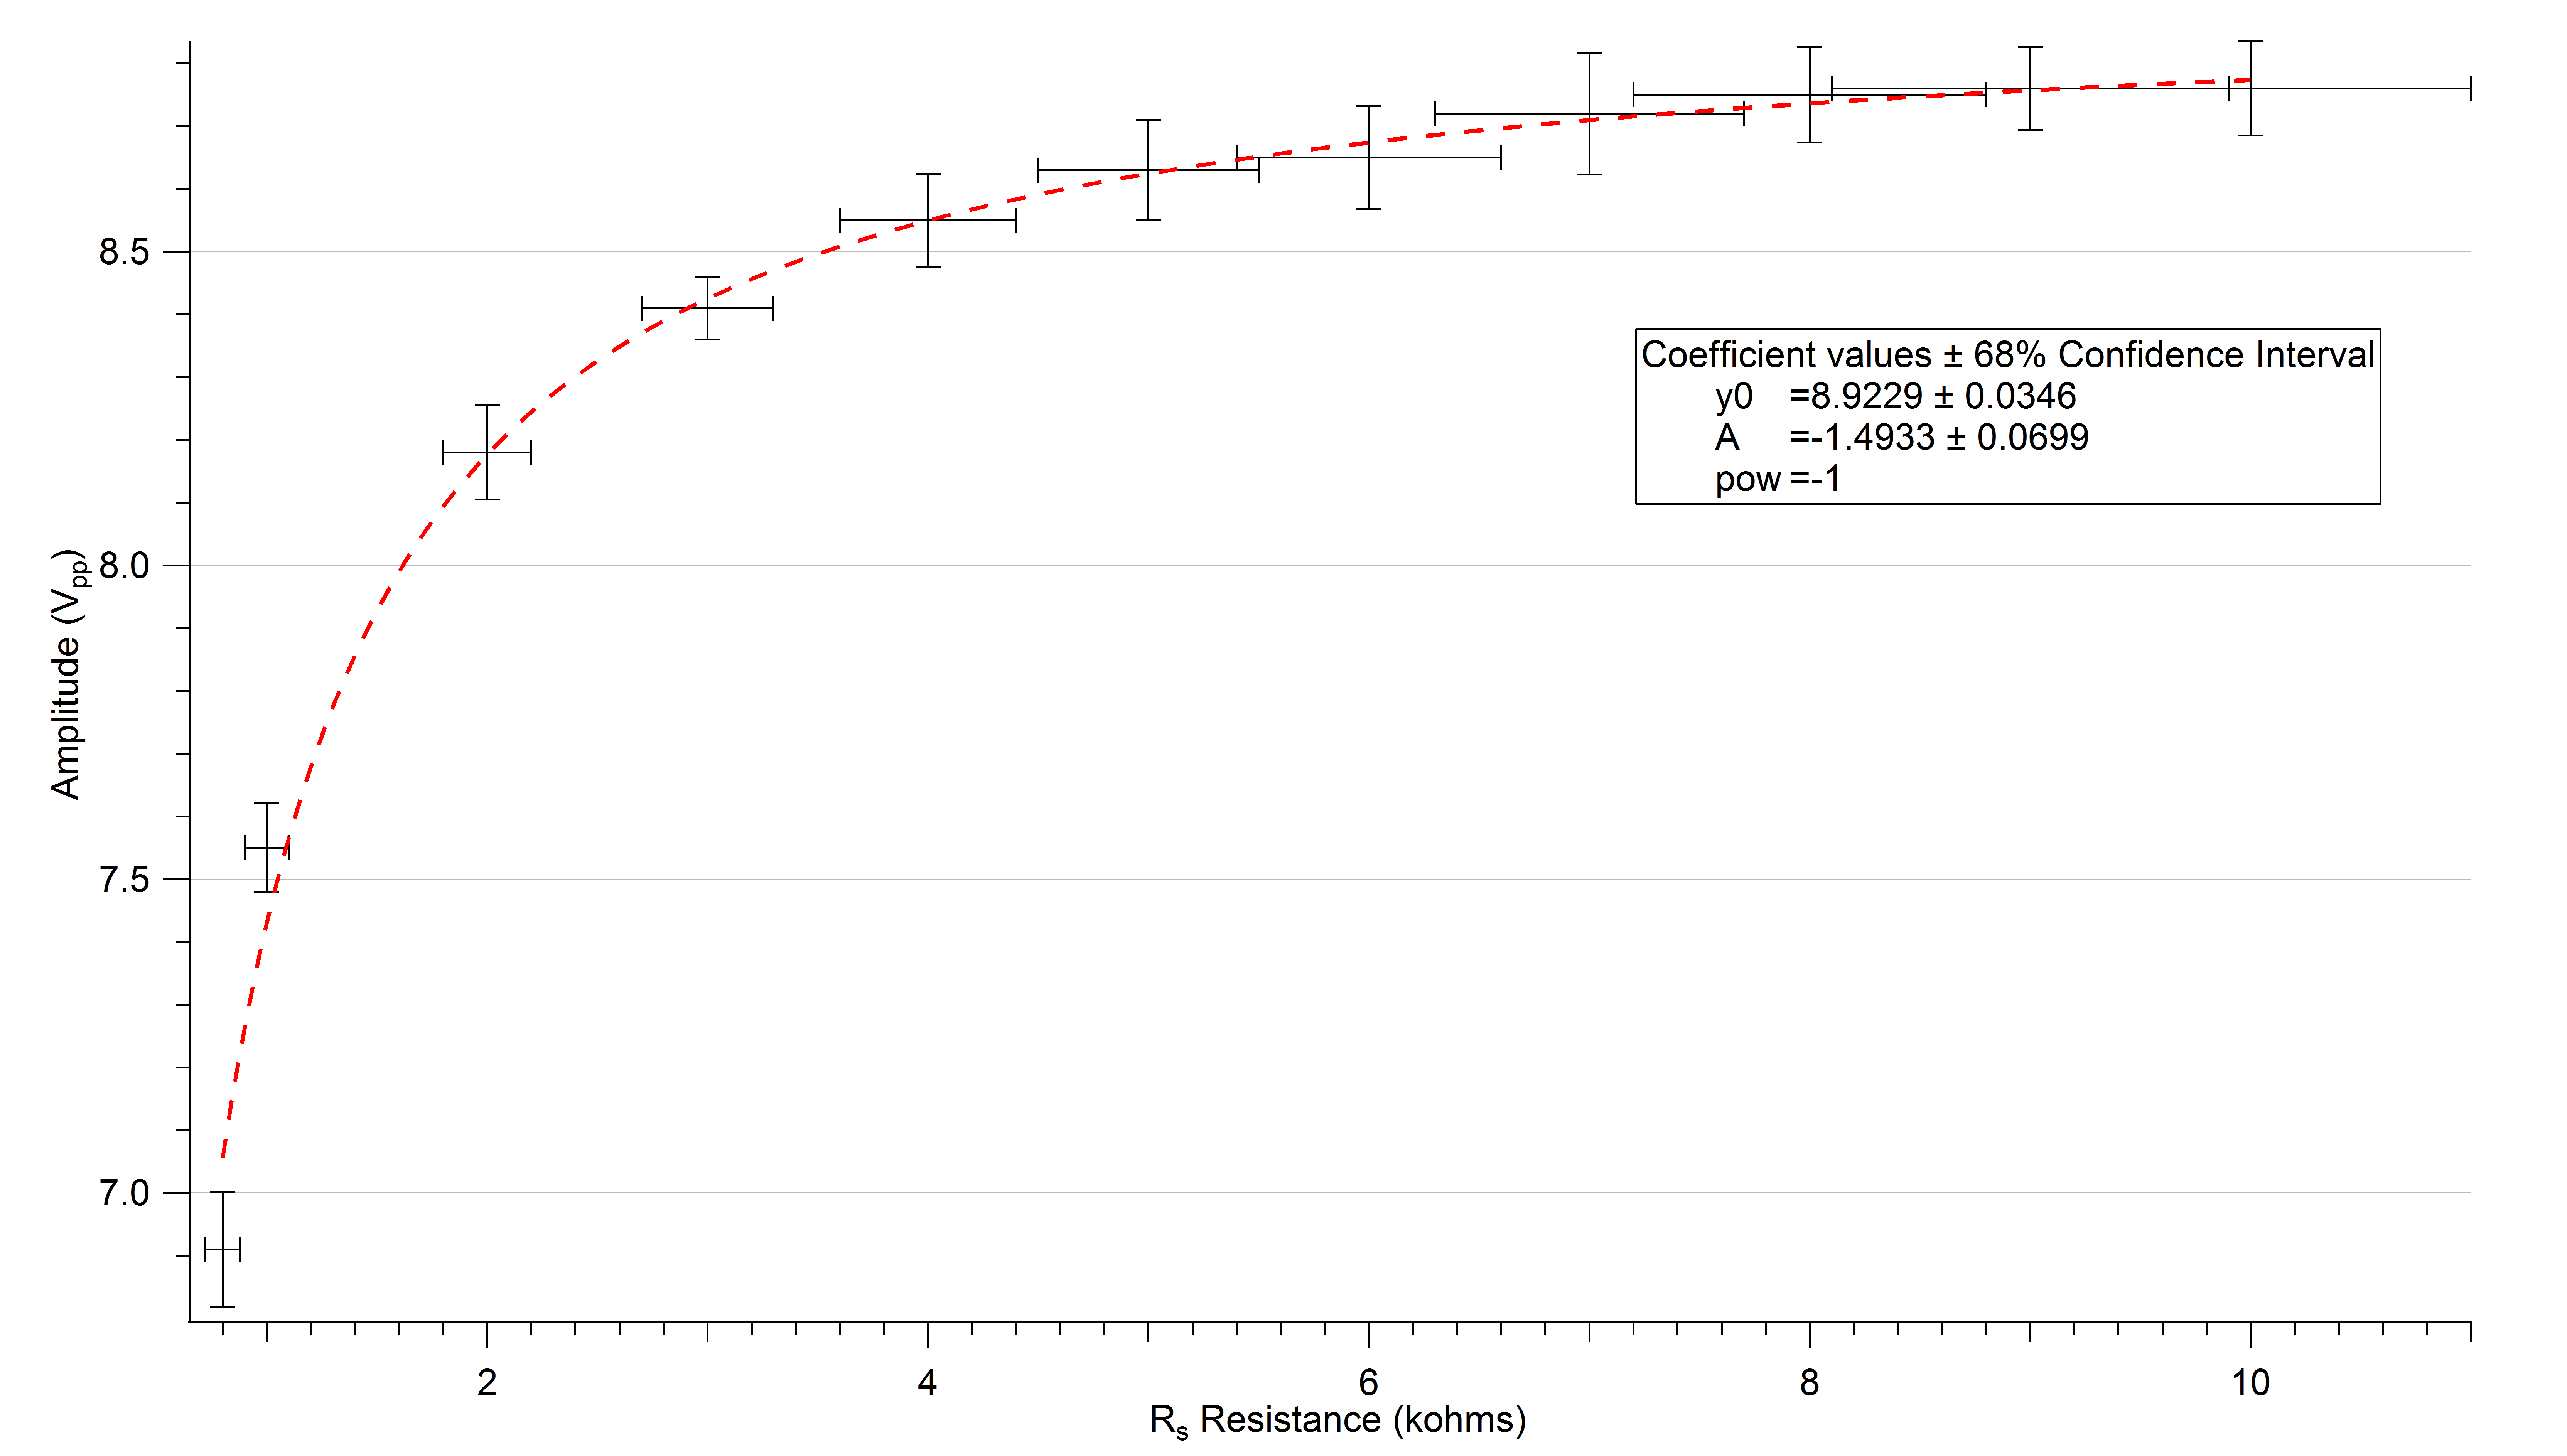
\includegraphics[scale=0.29]{Data/WienBridgeAmplitude.png}
\label{WBOAmplitude}
\end{figure}

As seen in the figures a power function fit of the experimental data generates great correspondence and agrees with the governing frequency equation in (3). Using the theoretical value of $4.7\mu F$ the respective frequency constant of proportionality is determined to be $33.86Hz/k\Omega$ which deviates from the measured value of $66.91\pm2.31 Hz/k\Omega$ by $49\%$. This deviation is large but can be associated to non-idealities associated with the utilized operational amplifier or load impedance.

The observed amplitude relationship serves to demonstrate the fact that operational amplifier gain does indeed have a frequency dependence and that higher frequencies produce lower gains. Since the wien bridge oscillator is very gain sensitive the associated frequency cut-off appears to occur much sooner then anticipated.
\pagebreak
\subsection{Triangle Wave Generator}%done

The visual examination of the triangle wave generator is illustrated in Figure \ref{TWGAmplitude}. The associated output frequency was measured at $1122Hz\pm 13Hz$ which deviated from the expected value of $1532Hz$ by $27\%$. 

\begin{figure}[H]
\centering
\caption{Triangle Wave Generator Amplitude Control}
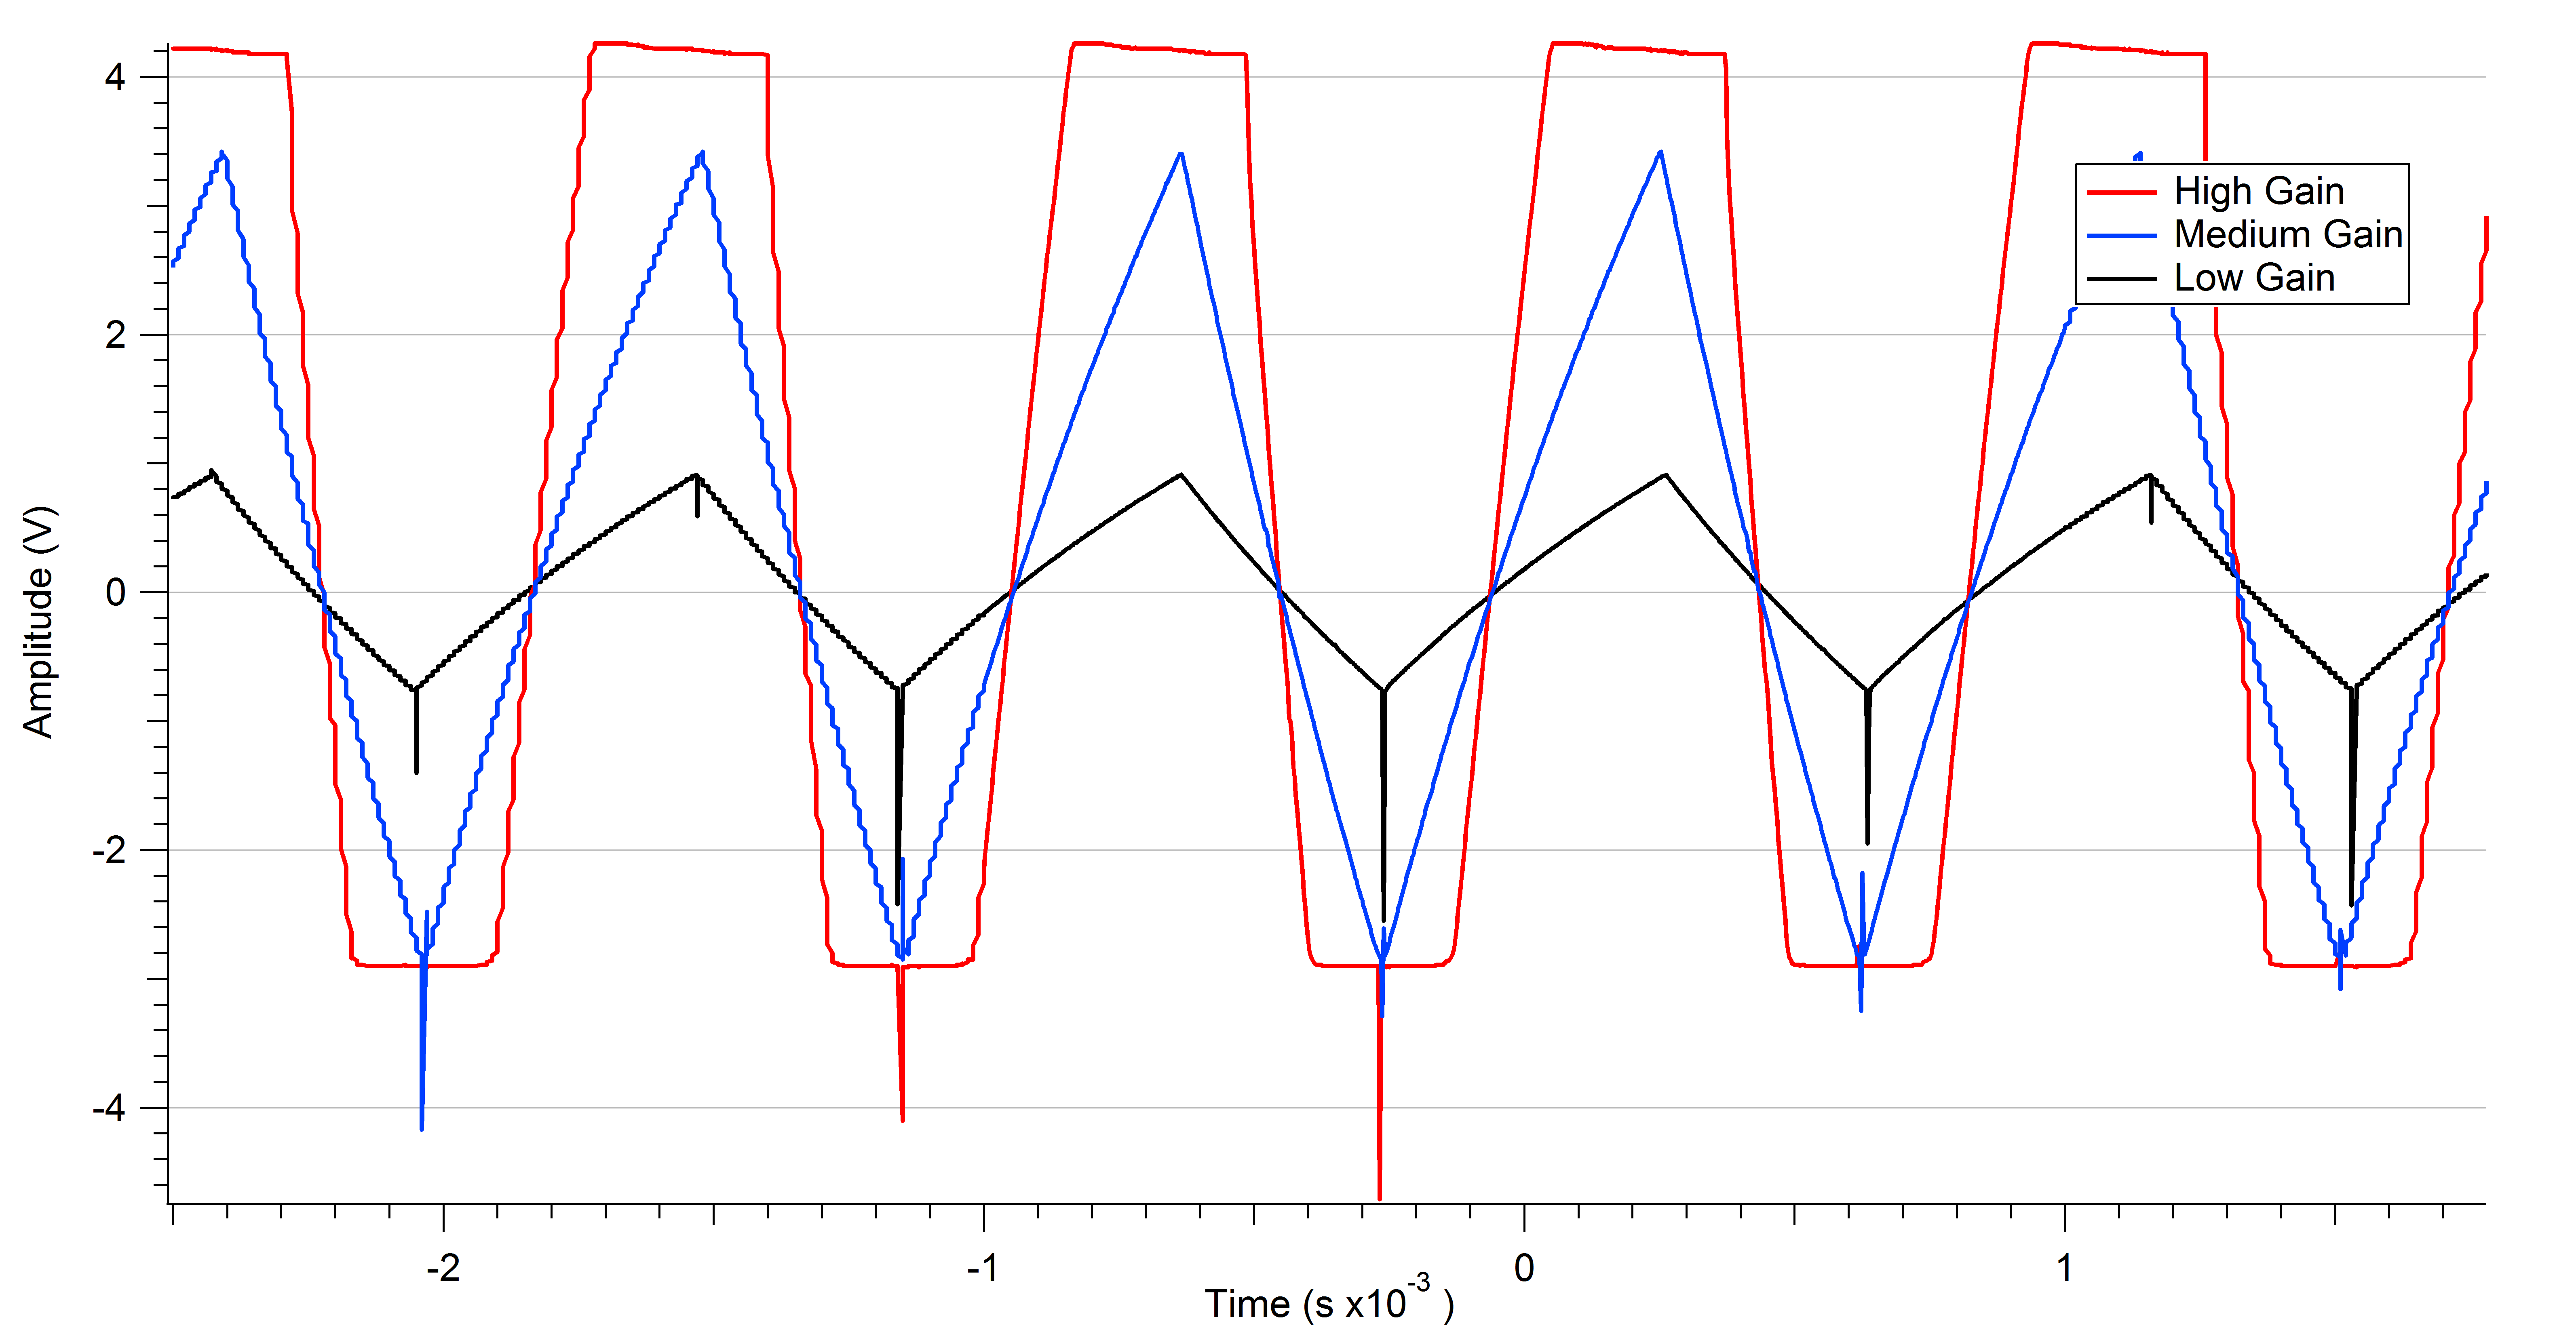
\includegraphics[scale=0.29]{Data/TriangleWaveGeneratorAmplitude.png}
\label{TWGAmplitude}
\end{figure}

From the figure the effect of $R_a$ on output amplitude is clearly shown to be in accordance with expectations. It is also observed that for very high setpoints the signal gets truncated due to the limiting supply voltage being used to operate the op-amps.
\pagebreak
\subsection{Three Phase Generation}%done

The results of the three phase generation accuracy test are illustrated in Figure \ref{ThreePhaseGenerationA} and show nearly linear frequency dependence over the tested range. 

\begin{figure}[H]
\centering
\caption{Three Phase Generation Accuracy}
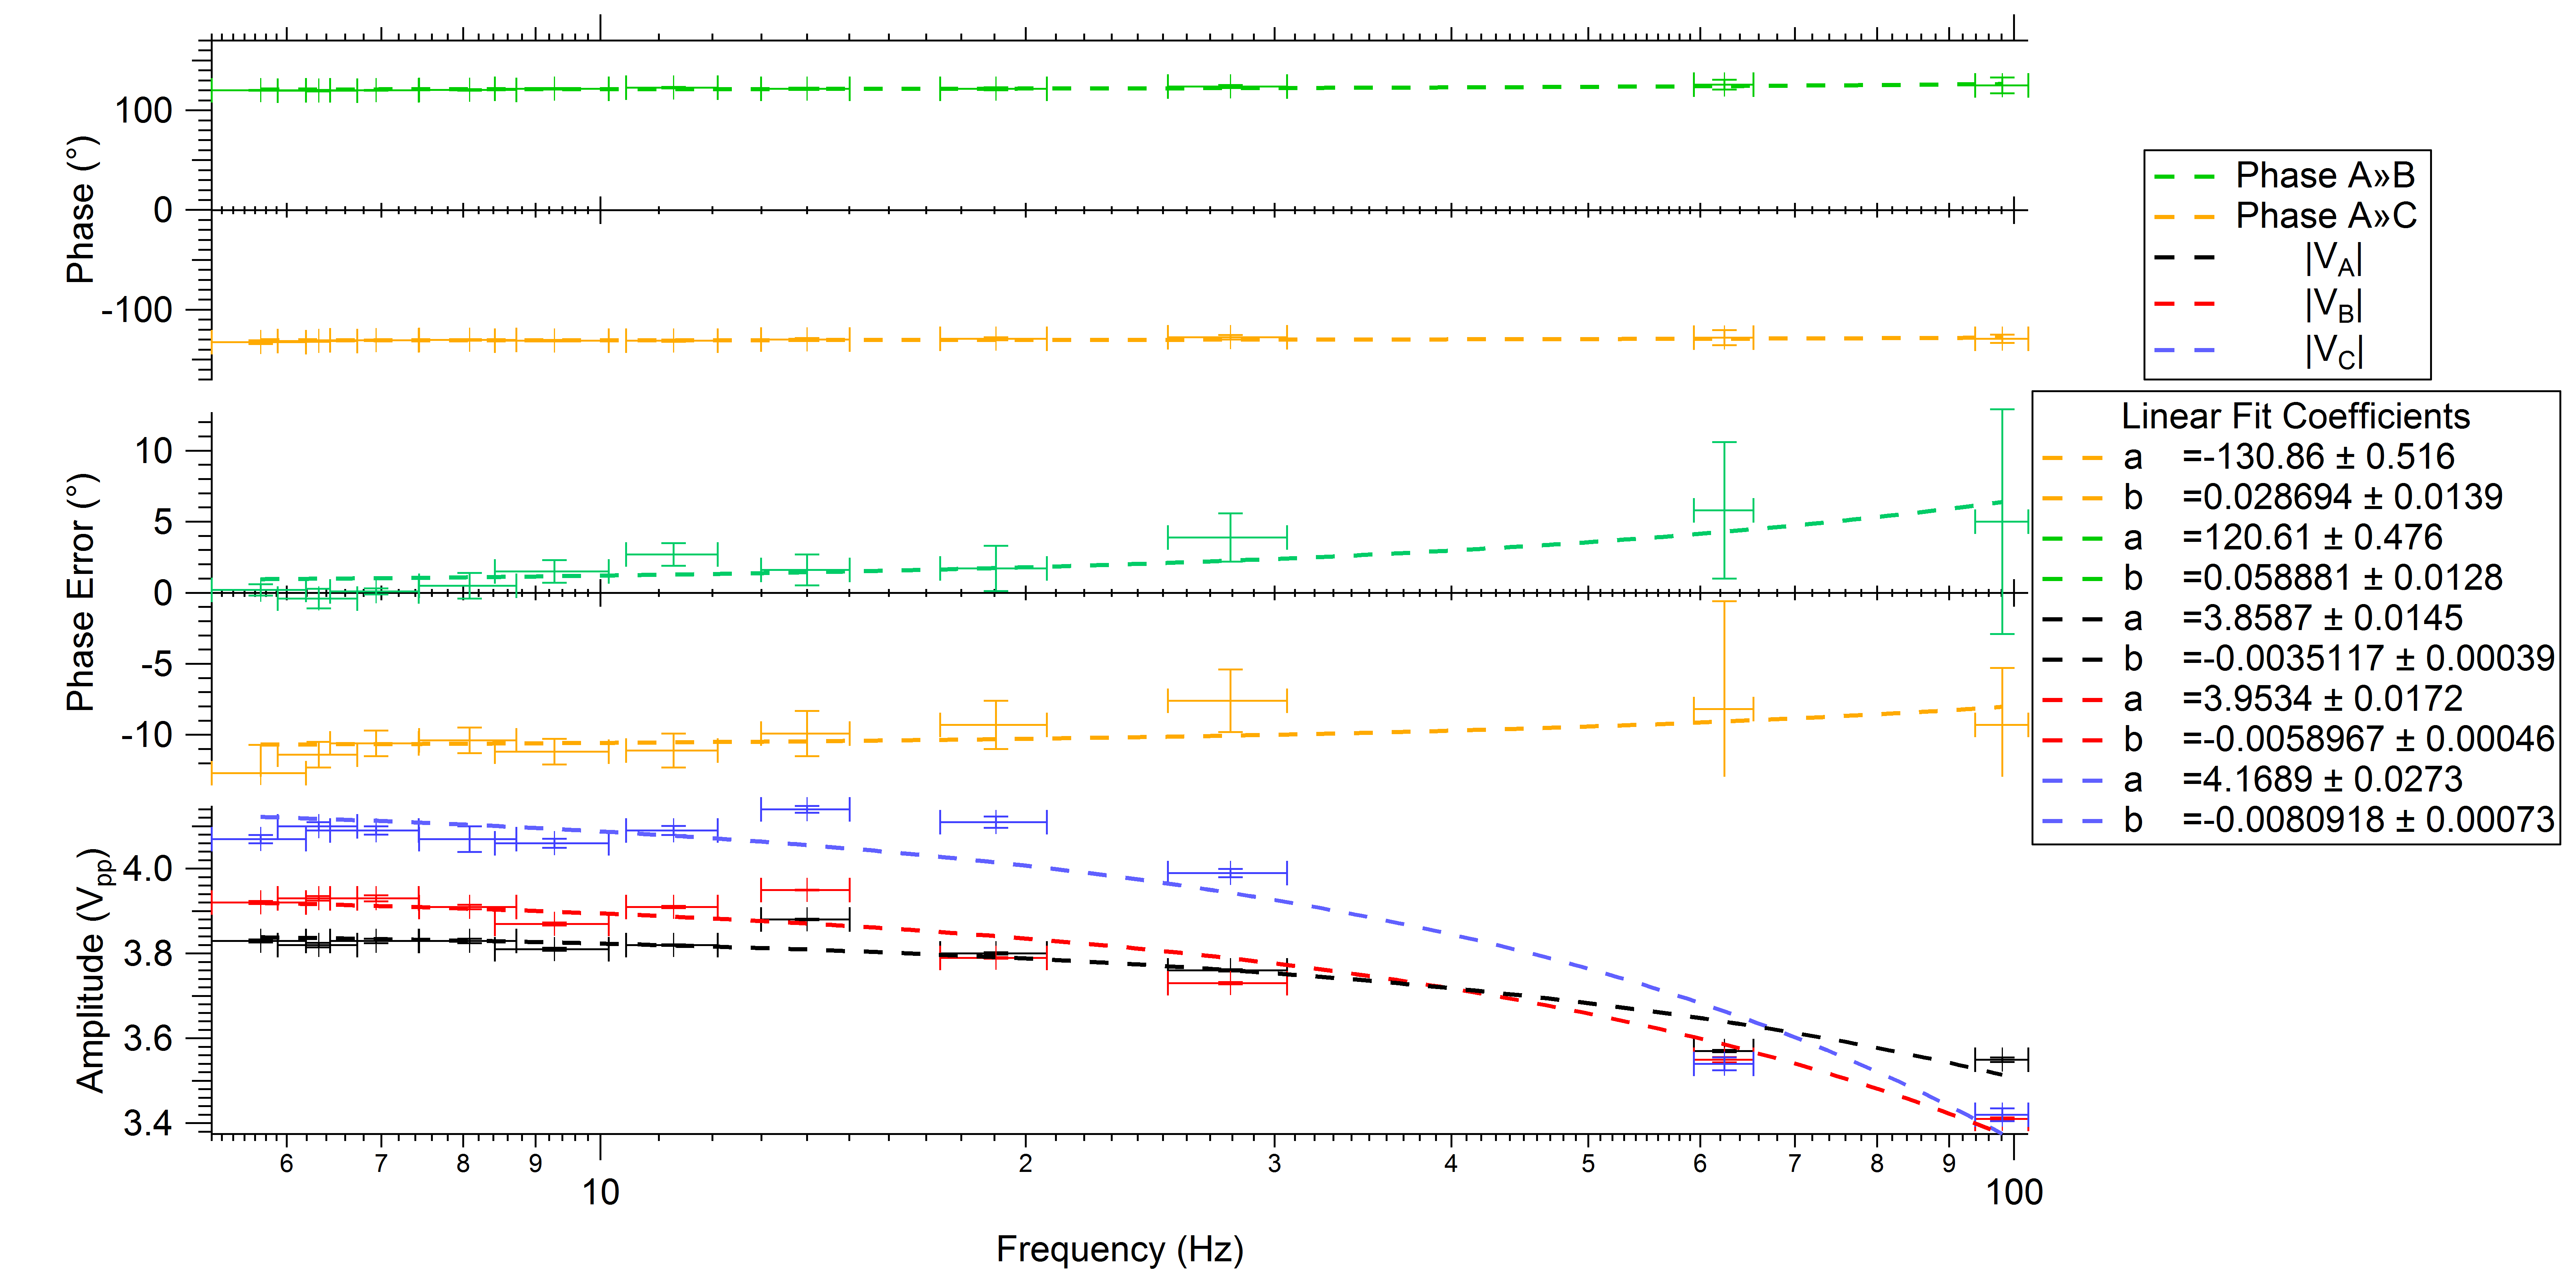
\includegraphics[scale=0.32]{Data/ThreePhaseGeneration.png}
\label{ThreePhaseGenerationA}
\end{figure}

In regards to the relative phase accuracy it was determined that PhaseAB measured at $120.61\pm 0.48^{\circ}$ and PhaseAC at $-130.86\pm 0.52^{\circ}$. Thus taking phase A as a reference it was observed that Phase C contained the largest deviations from expectations at $7\%$ error which is quite reasonable. It was also observed that near the high frequency end of the spectrum phase deviations begin to increase slightly. This is most likely associated with the increased instability present within the wien bridge output waveform as described in the previous section. Acting as further evidence to this theory the associated magnitude response of the output phases with respect to frequency also show significant reductions near the higher end of the frequency range. 
\subsection{Control Pulse Generation}%done

Results obtained from the direct analysis of the two pulse control sequences on the project prototype are described in detain in the following sections.

\subsubsection{Trapezoidal Pulse Width Modulation}%done

Referencing the input sine waveforms with the DC signal introduced a delay between respective peaks which was controlled through alteration of $R_d$. The results of the effect of this delay on phase spacing is illustrated in Figure \ref{PhaseDelay} and shows that with higher delay it becomes impossible for phases to overlap with the compromise being smaller motor torque periods.

\begin{figure}[H]
\centering
\caption{TPWM Pulse Width Delay Phase Accuracy}
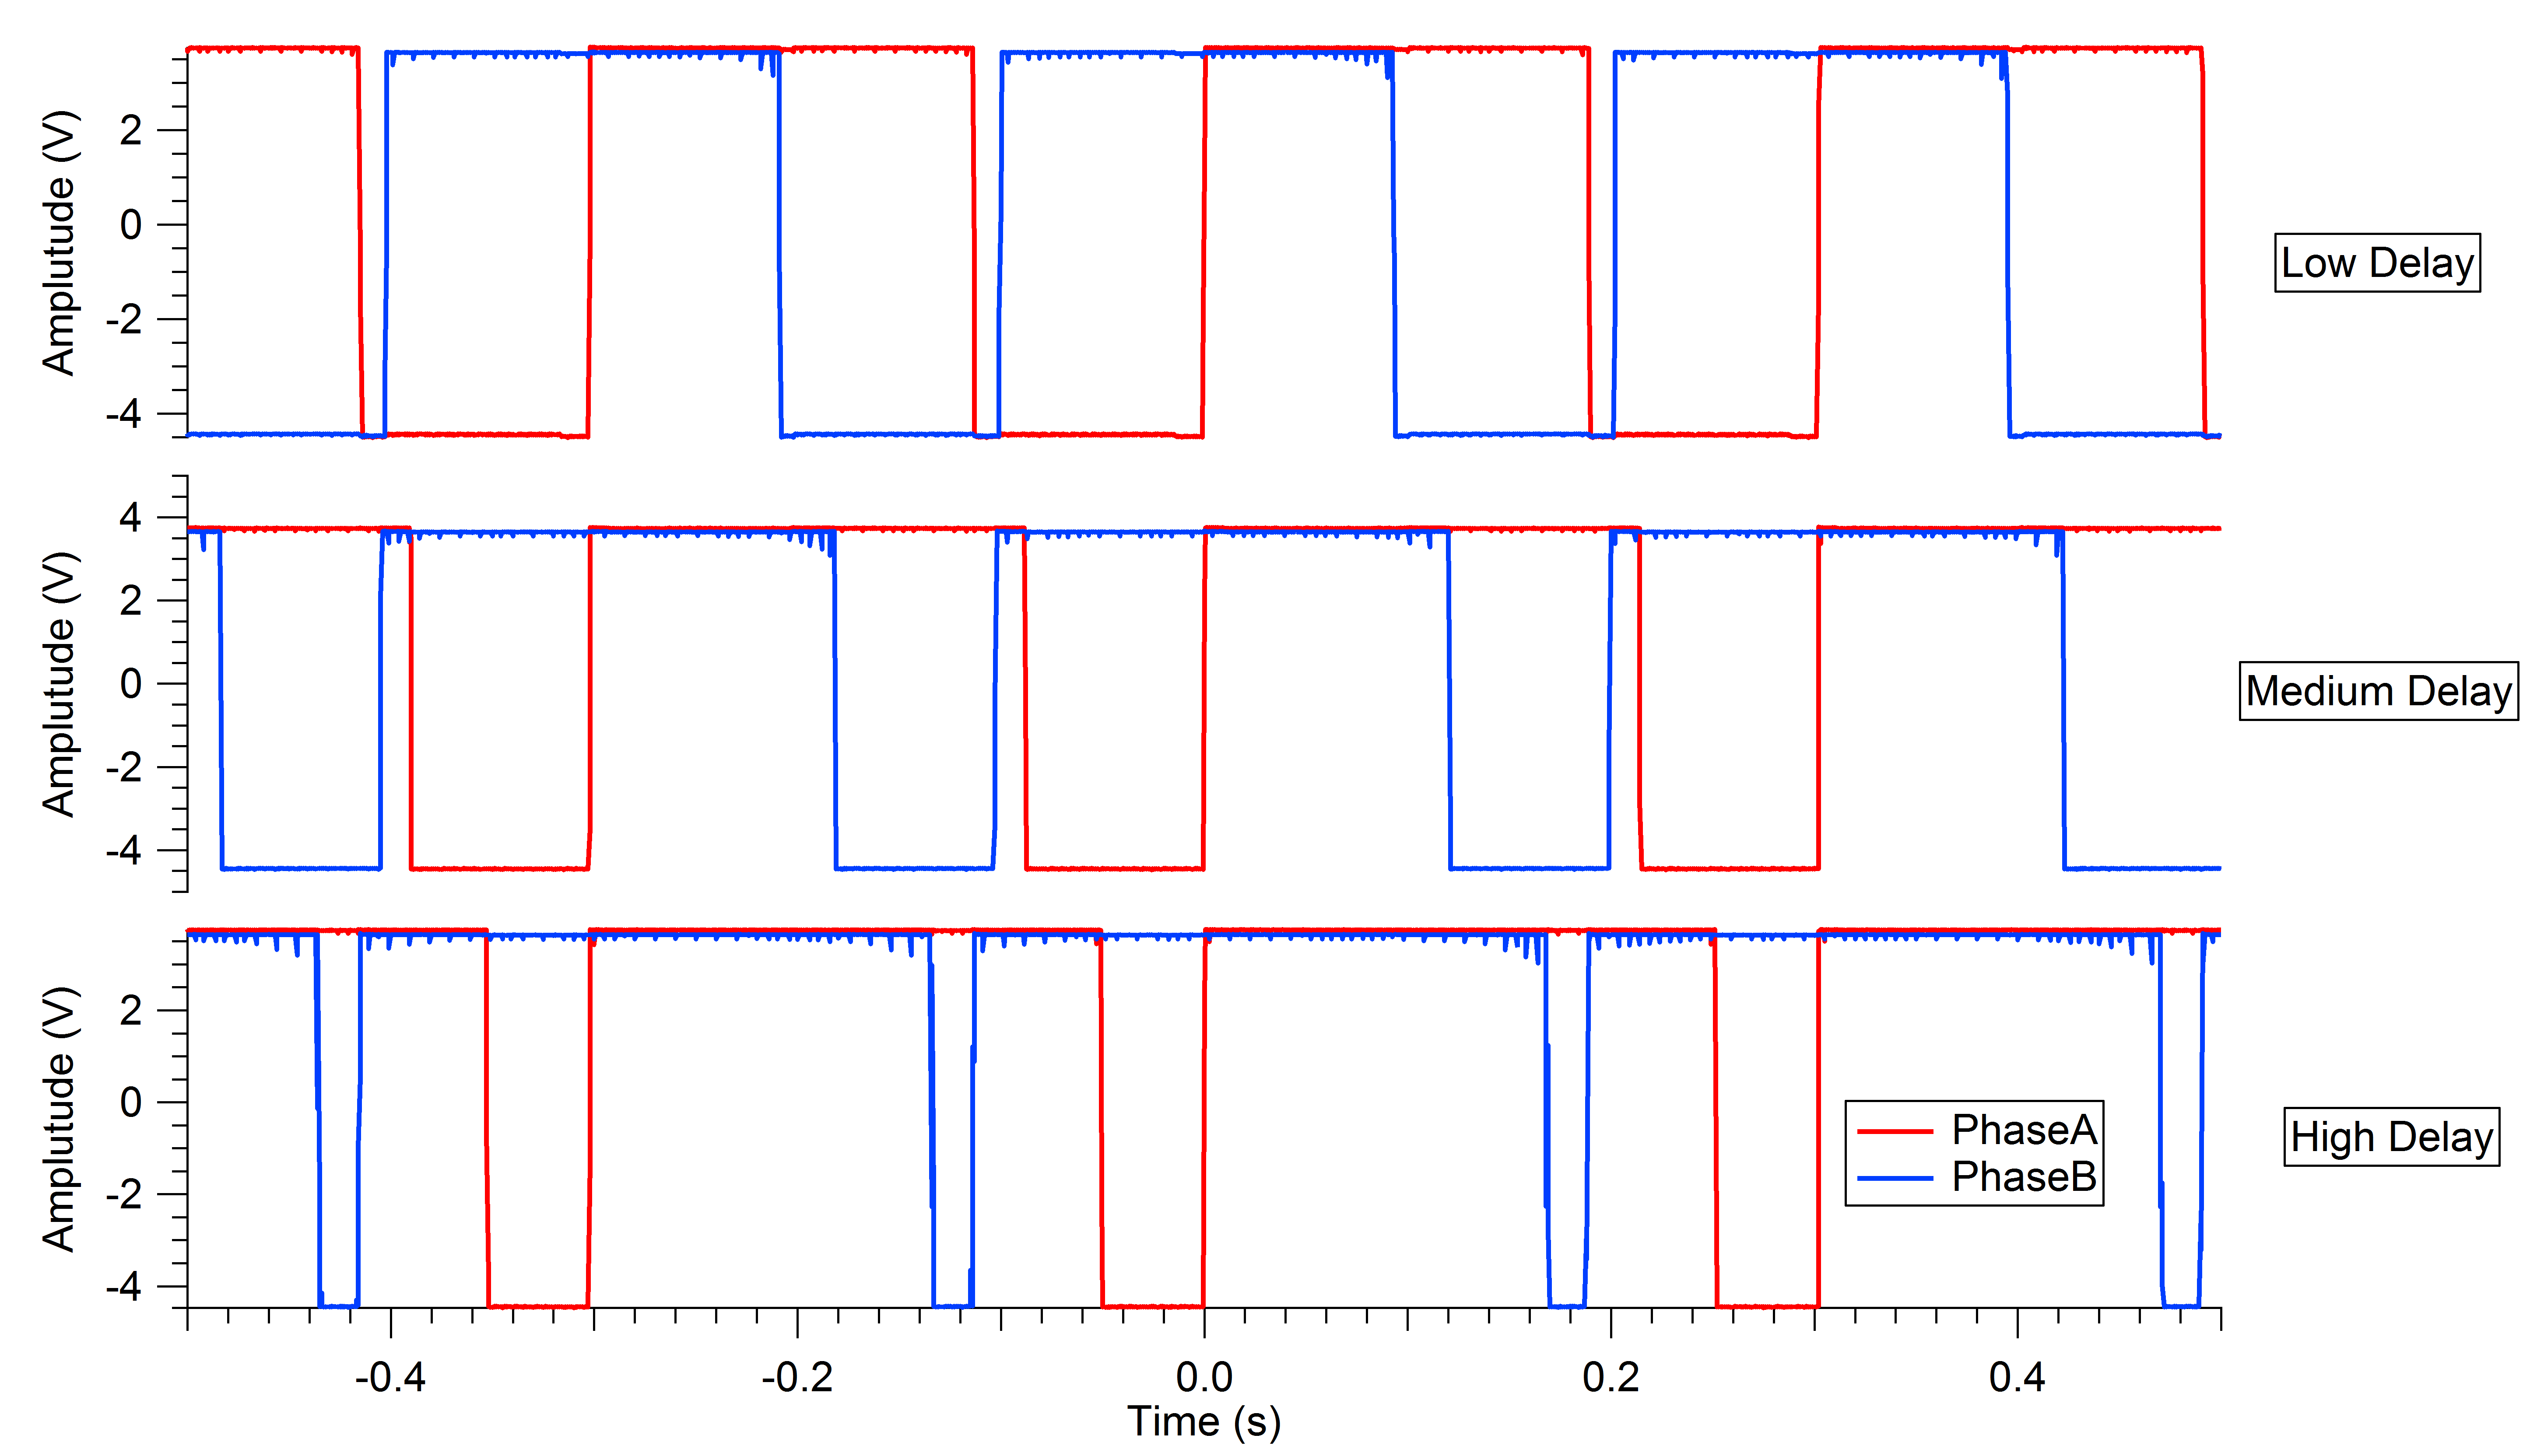
\includegraphics[scale=0.32]{Data/TPWM_PulsePhaseDelay.png}
\label{PhaseDelay}
\end{figure}

The secondary product of this delay is modulation and the results of the effect is illustrated in Figure \ref{PhaseDelayMod} and shows that with larger delays the motor is active for longer intervals hence producing more torquing power.

\begin{figure}[H]
\centering
\caption{TPWM Pulse Width Modulation through $R_d$}
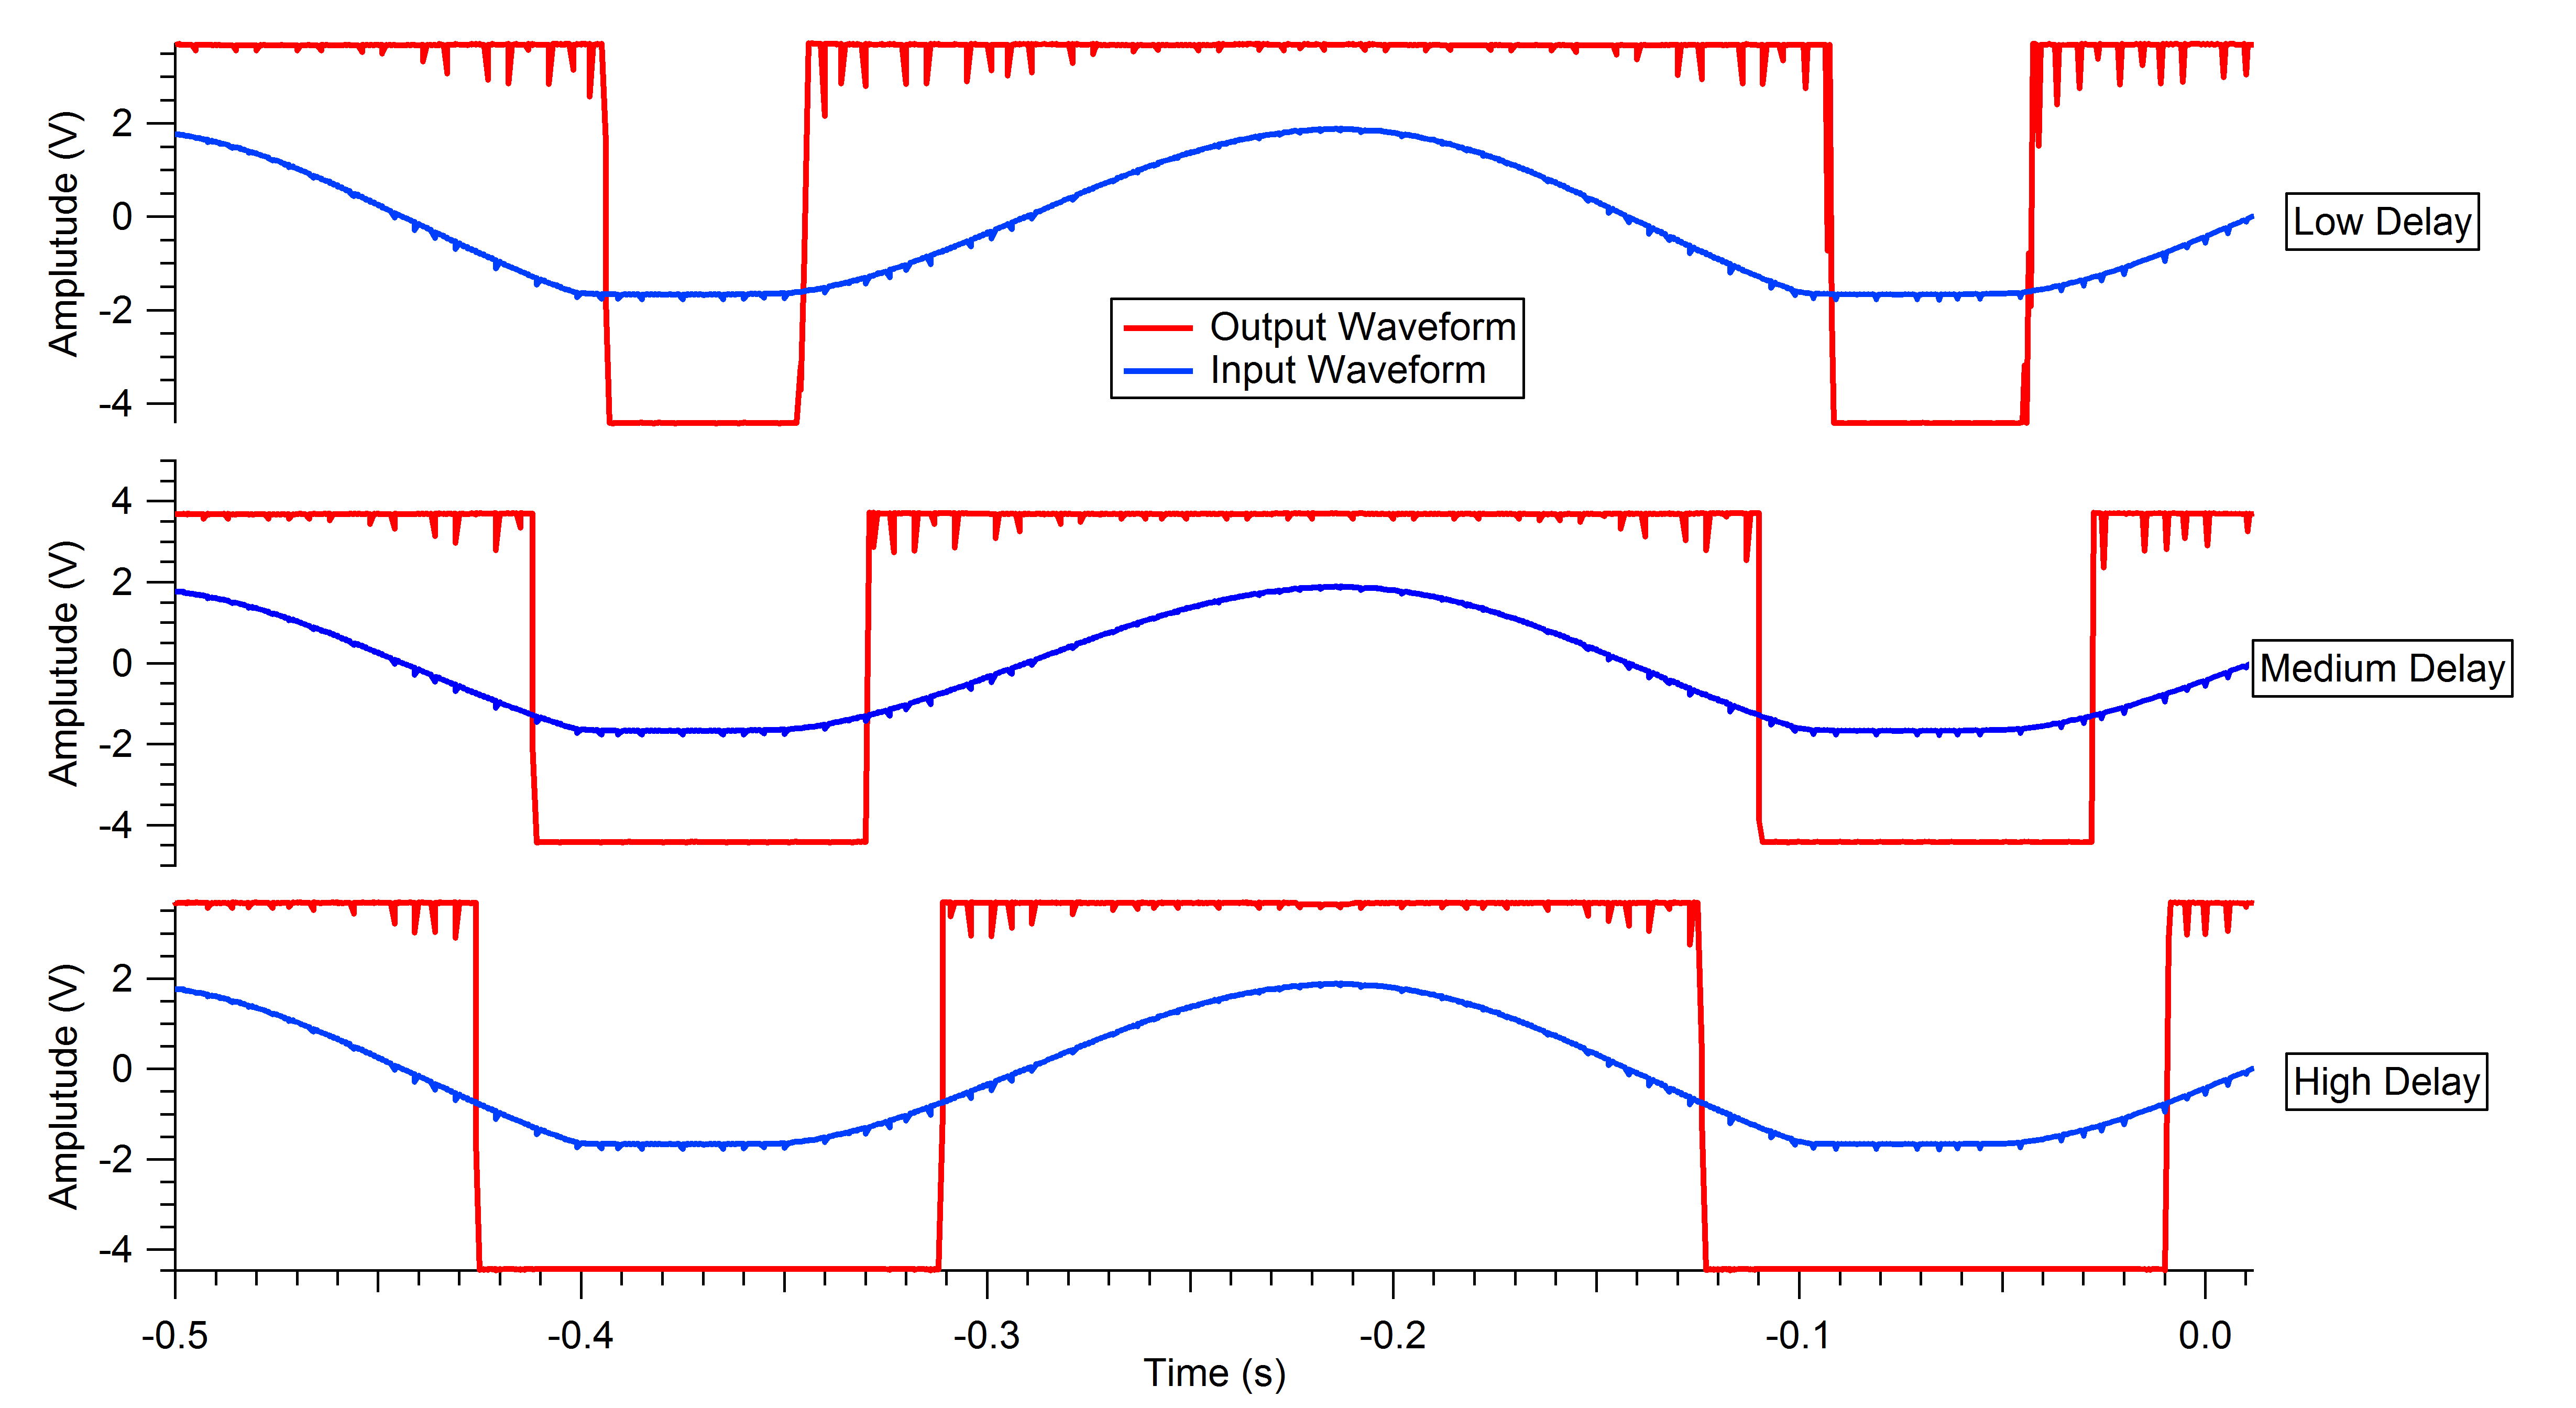
\includegraphics[scale=0.42]{Data/TPWM_PulseDelay.png}
\label{PhaseDelayMod}
\end{figure}

Lastly the effect of superimposing the triangle waveform on the pulse is illustrated in Figure \ref{TPWMA} and shows that under the condition of high modulation the waveform closely resembles the operation of a true TPWM signal. This also allows for complete control of the output current of the H-Bridge through direct changes in average pulse output strength.

\begin{figure}[H]
\centering
\caption{TPWM Amplitude Modulation through $R_a$}
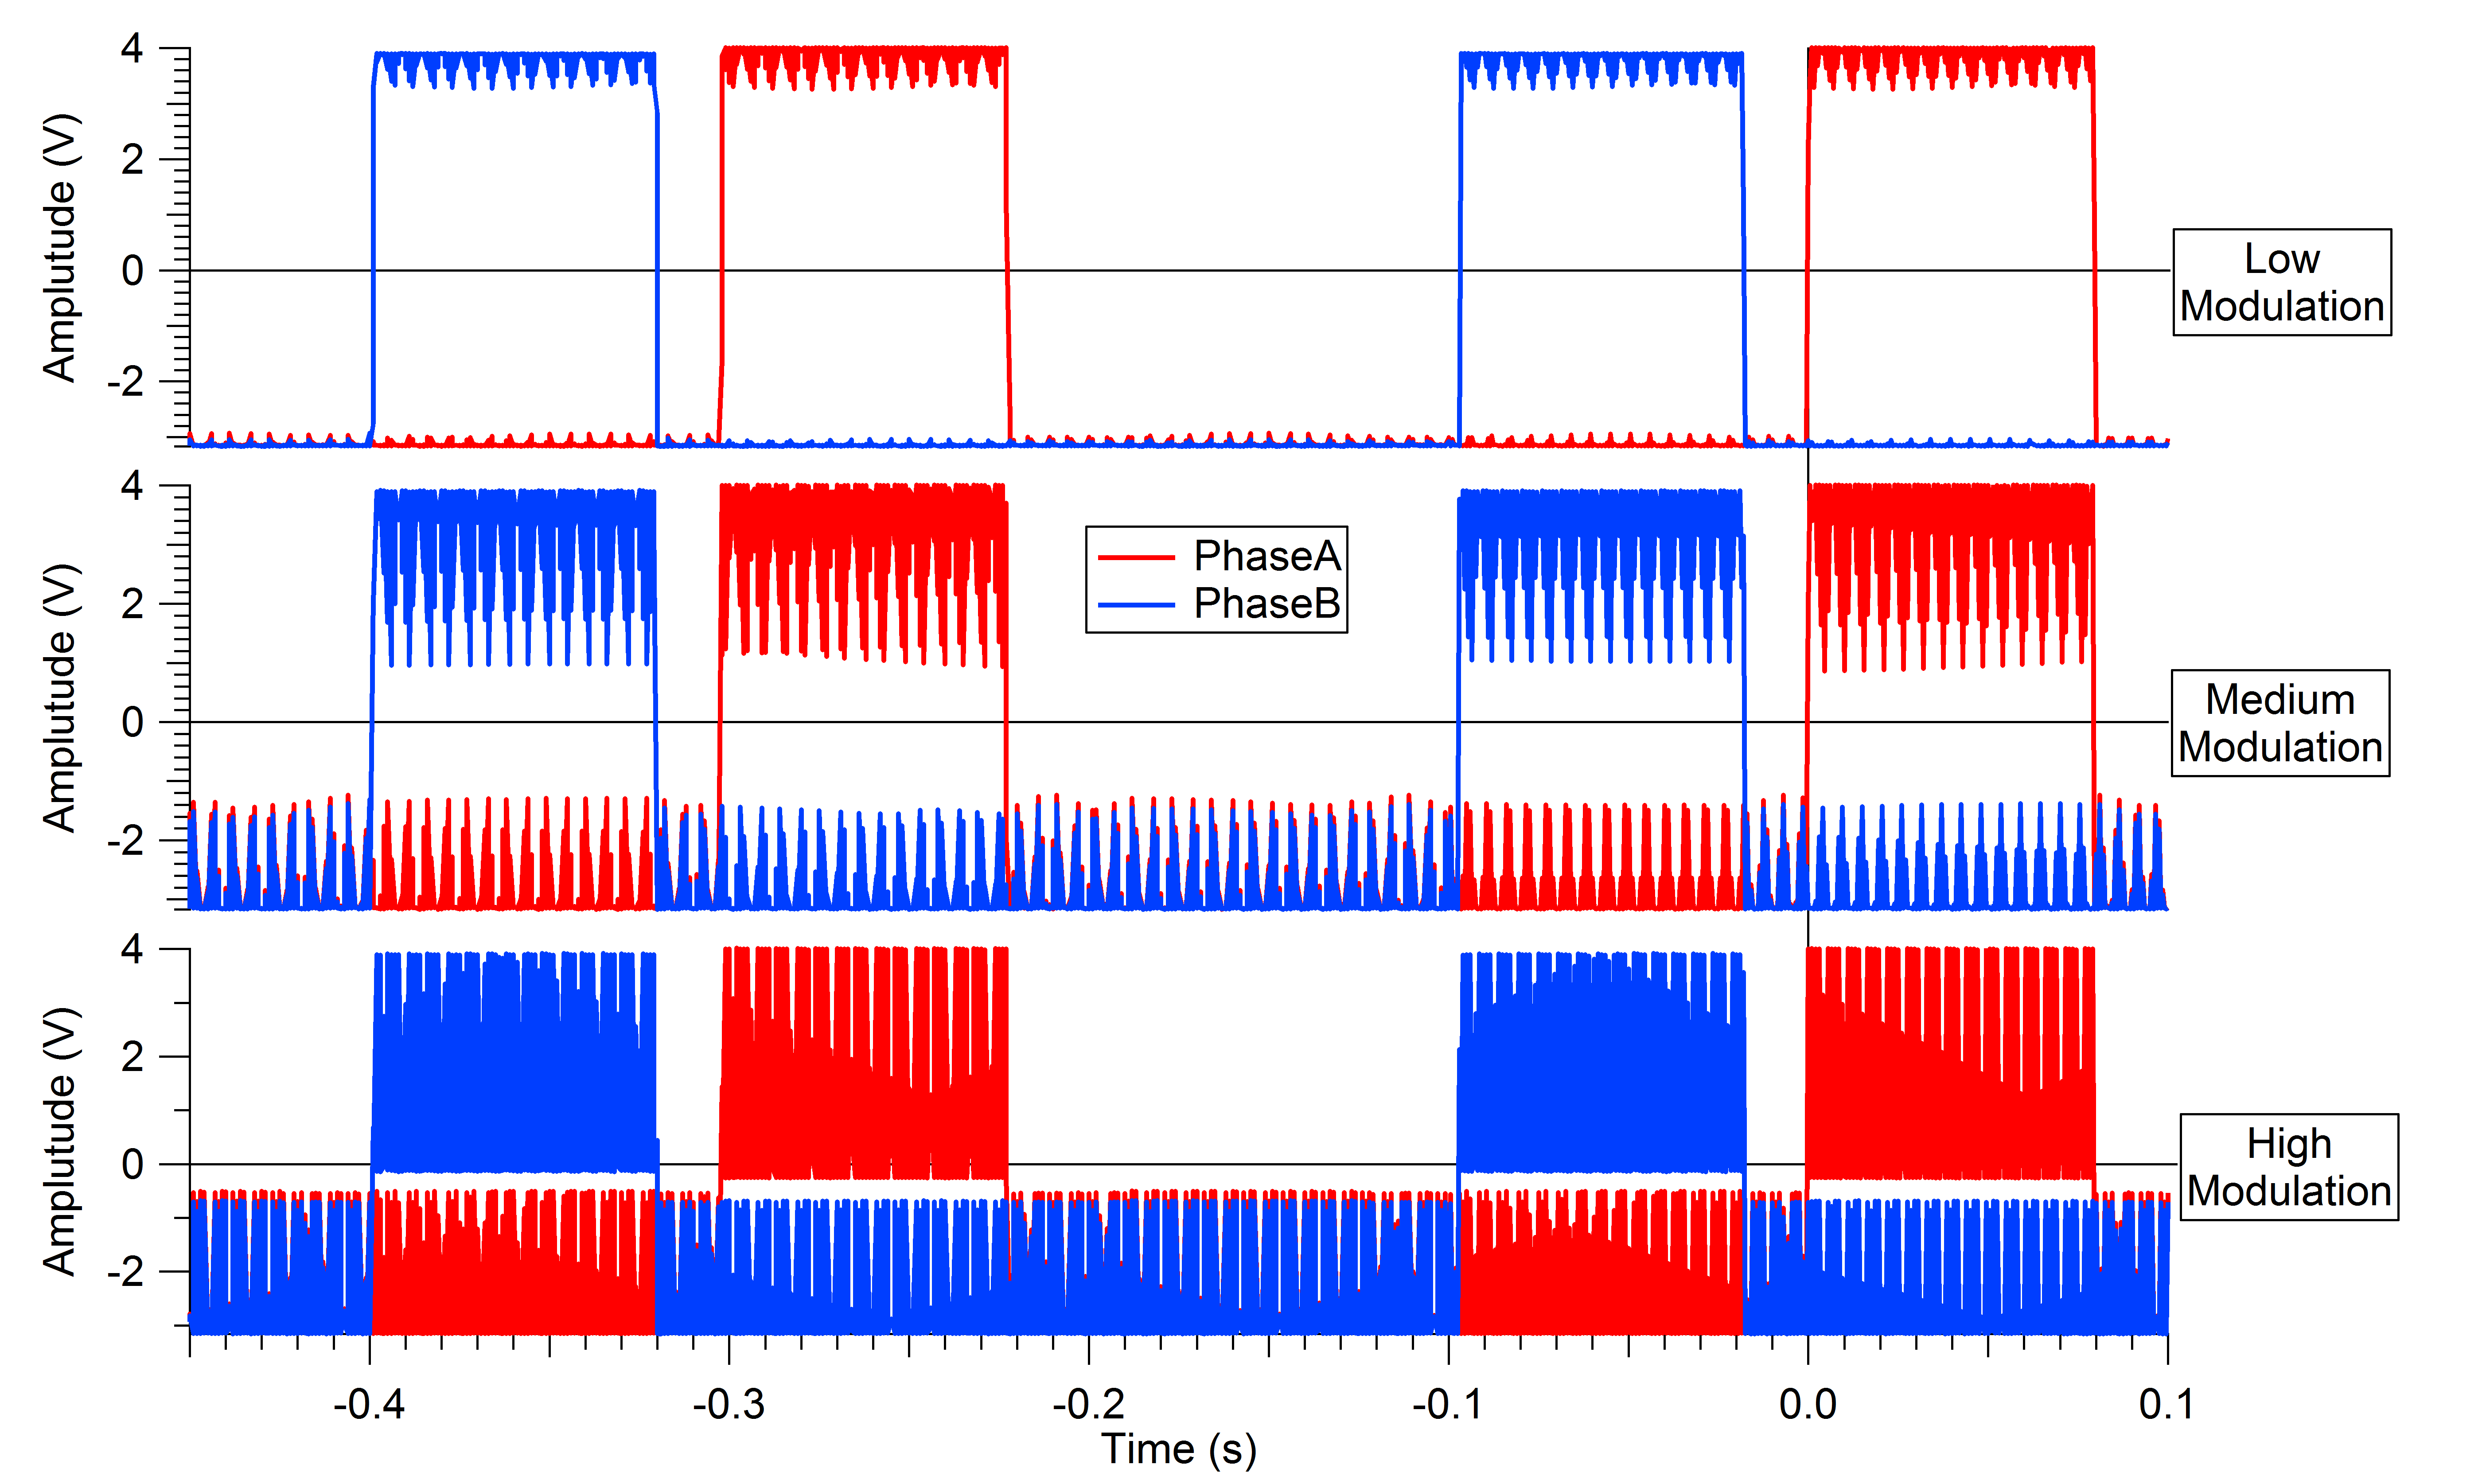
\includegraphics[scale=0.38]{Data/TPWM_PulseModulation.png}
\label{TPWMA}
\end{figure}

\subsubsection{Sinusoidal Pulse Width Modulation}%done

As the fundamental purpose of SPWM generation is to approximate the sine waveform using pulses, the examination of the effectiveness of the circuit begins with a look at the accuracy of this approximation. Figure \ref{SPWM_Accuracy} illustrates the progression of the input sinewave into a PWM waveform. This waveform is then filtered through a mathematically modeled low pass filter and the result is displayed on the bottom.

\begin{figure}[H]
\centering
\caption{SPWM Accuracy Examination}
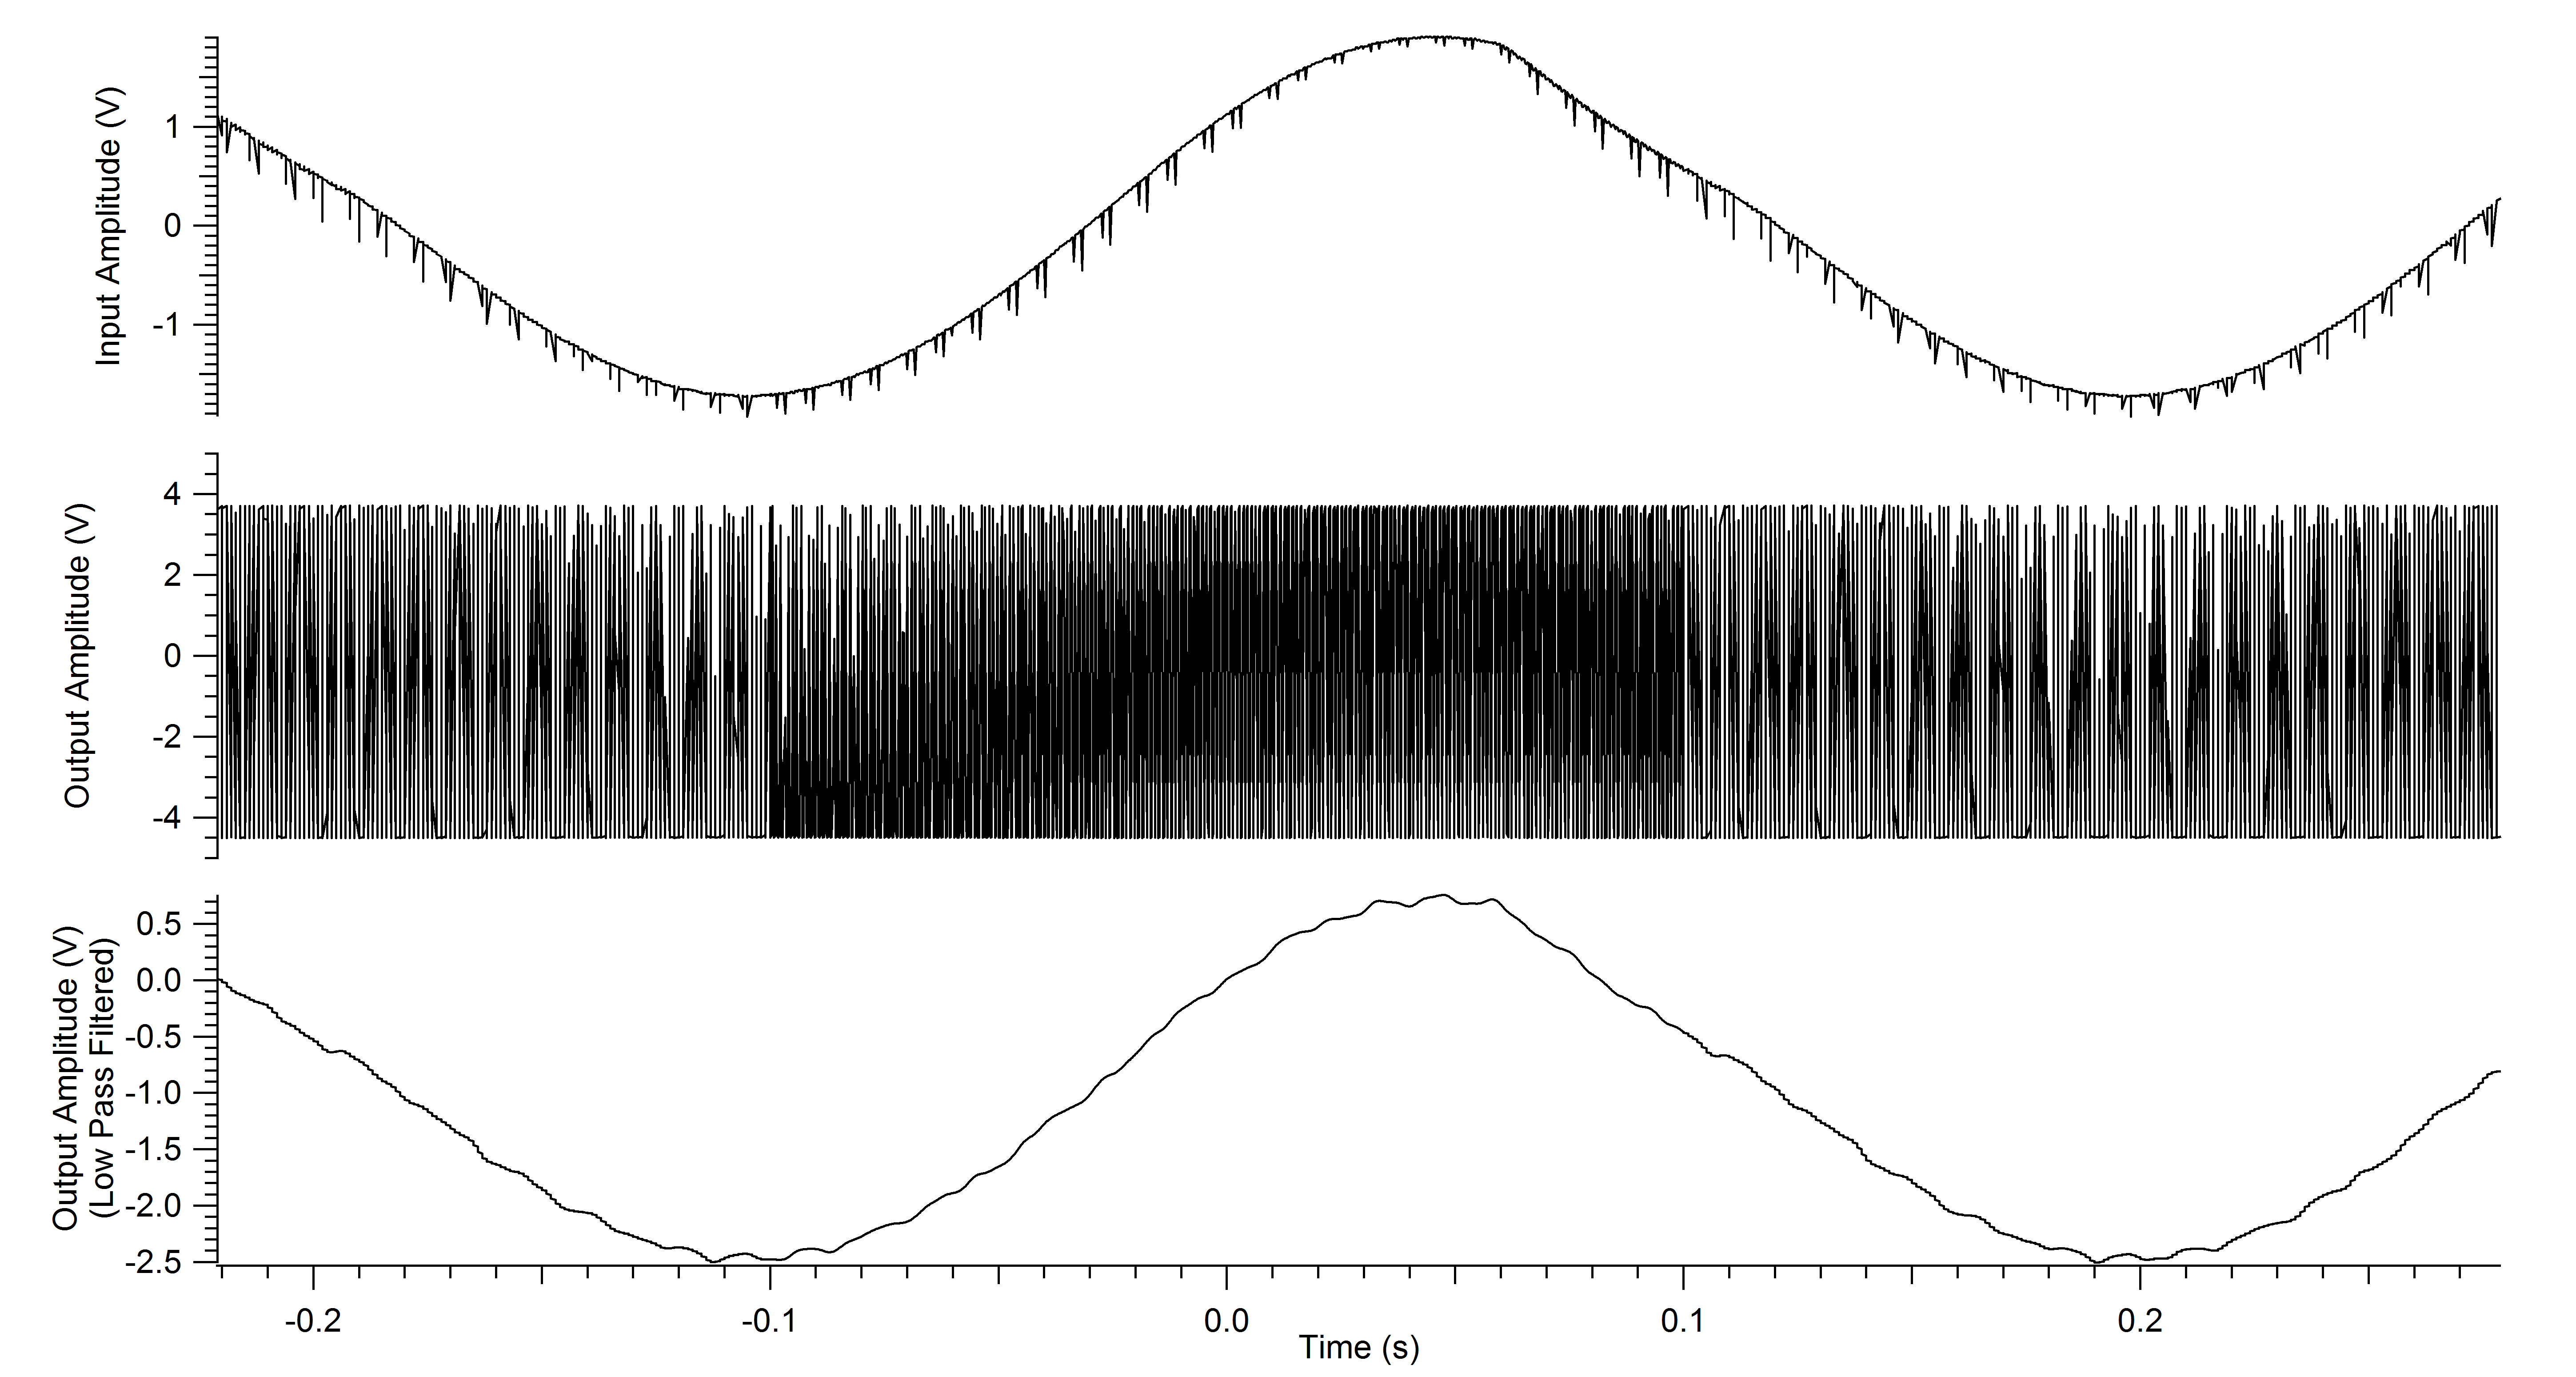
\includegraphics[scale=0.32]{Data/SPWM_Accuracy.png}
\label{SPWM_Accuracy}
\end{figure}

Clearly the pulse modulated approximation is successful in modeling the true behavior of the waveform. Next the effect of current control is examined. Figure \ref{SPWM_TriangleWaveModulation} demonstrates the effect of altering the amplitude of the triangle waveform and its associated result on SPWM amplitude.

\begin{figure}[H]
\centering
\caption{Sinusoidal Pulse Width Modulation}
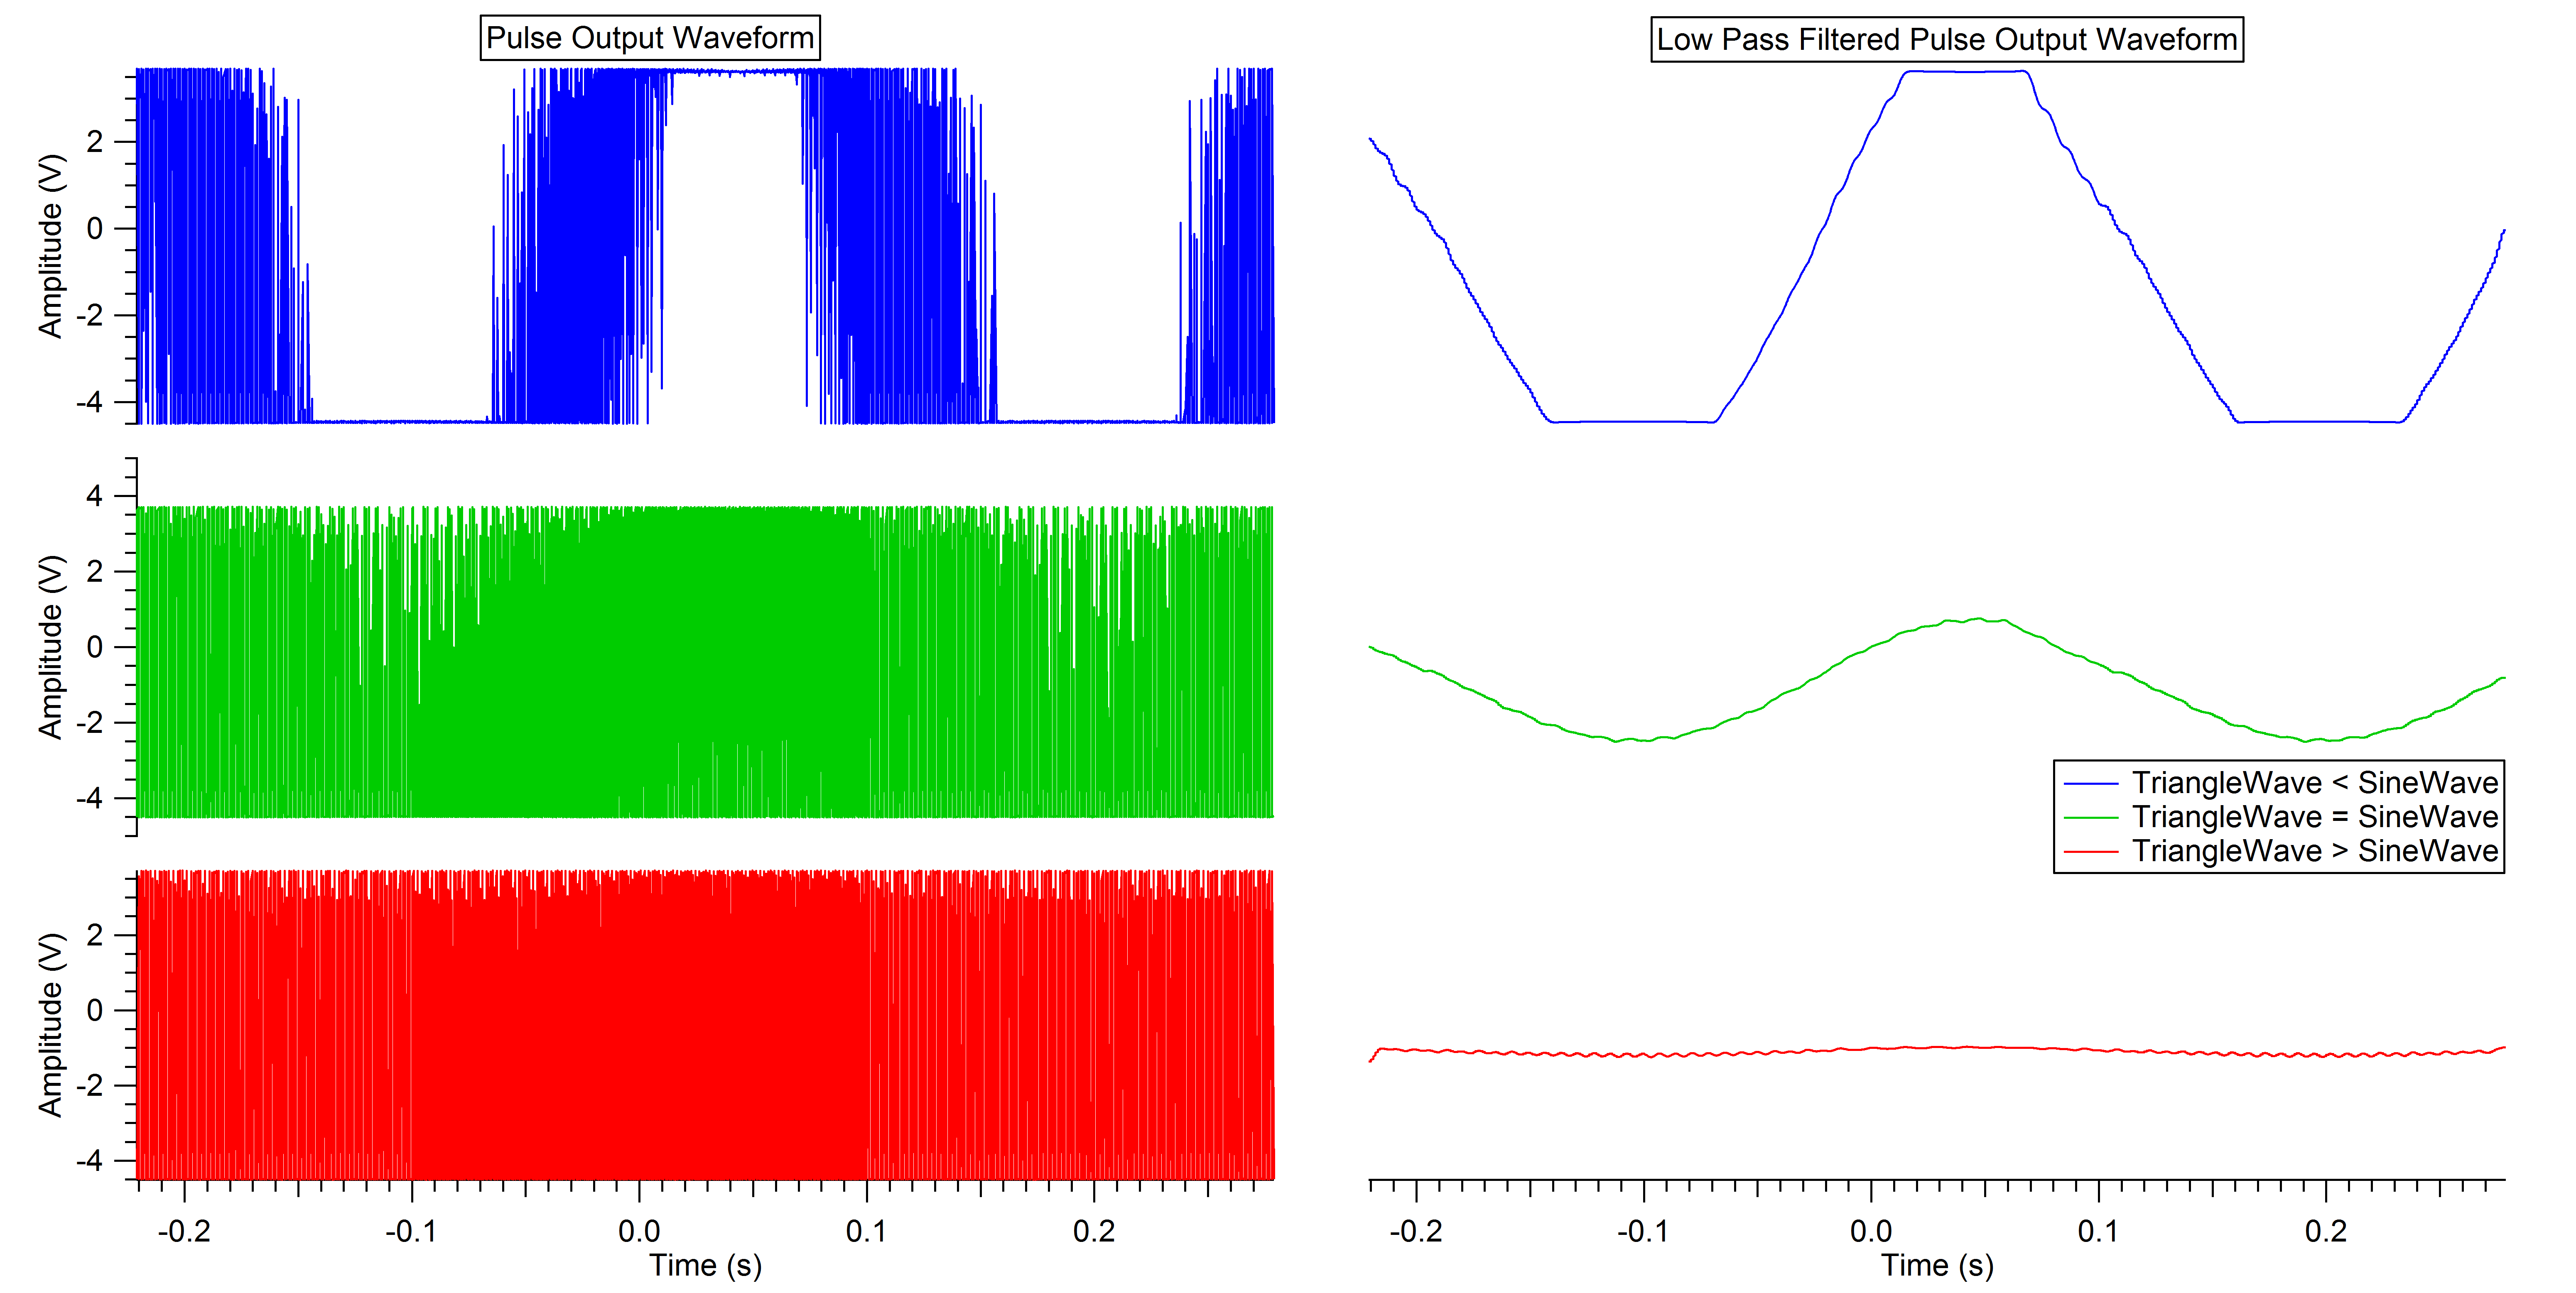
\includegraphics[scale=0.32]{Data/SPWM_TriangleWaveModulation.png}
\label{SPWM_TriangleWaveModulation}
\end{figure}

From the figure two important realizations can be made. First for the case of having the triangle waveform amplitude equal and above the sine waveform amplitude the resultant PWM pulses produce an average amplitude response that varies from low to high and as such can be used to regulate current flow through the H-bridge as desired. The second realization is that for the case of Triangle wave amplitude less then the sine wave amplitude the resulting filtered PWM signal resembles that of a Trapezoid. This was in fact an unexpected consequence caused by the limiting amplitude response of the utilized operational amplifiers. Regardless however it serves as another means of TPWM simulated control that is in fact an improvement upon the TPWM approximation that was intentionally generated as it contains the slightly tapered transition region iconic to trapezoidal pulse width modulation.
\subsection{Measured Motor Current Waveform}%done

The most meaningful method of verifying correct operation of the controller is through direct observation of the spinning of the motor itself. After having connected the "EMAX" motor to the controller output the results were a resounding success. Current waveforms were recorded for both modes of operation and illustrated in Figures~\ref{SPWM_Currentpng}~and~\ref{TPWM_Current} for the case of a spinning motor and a still motor (rotor held fixed).

\begin{figure}[H]
\centering
\caption{SPWM Current Waveform}
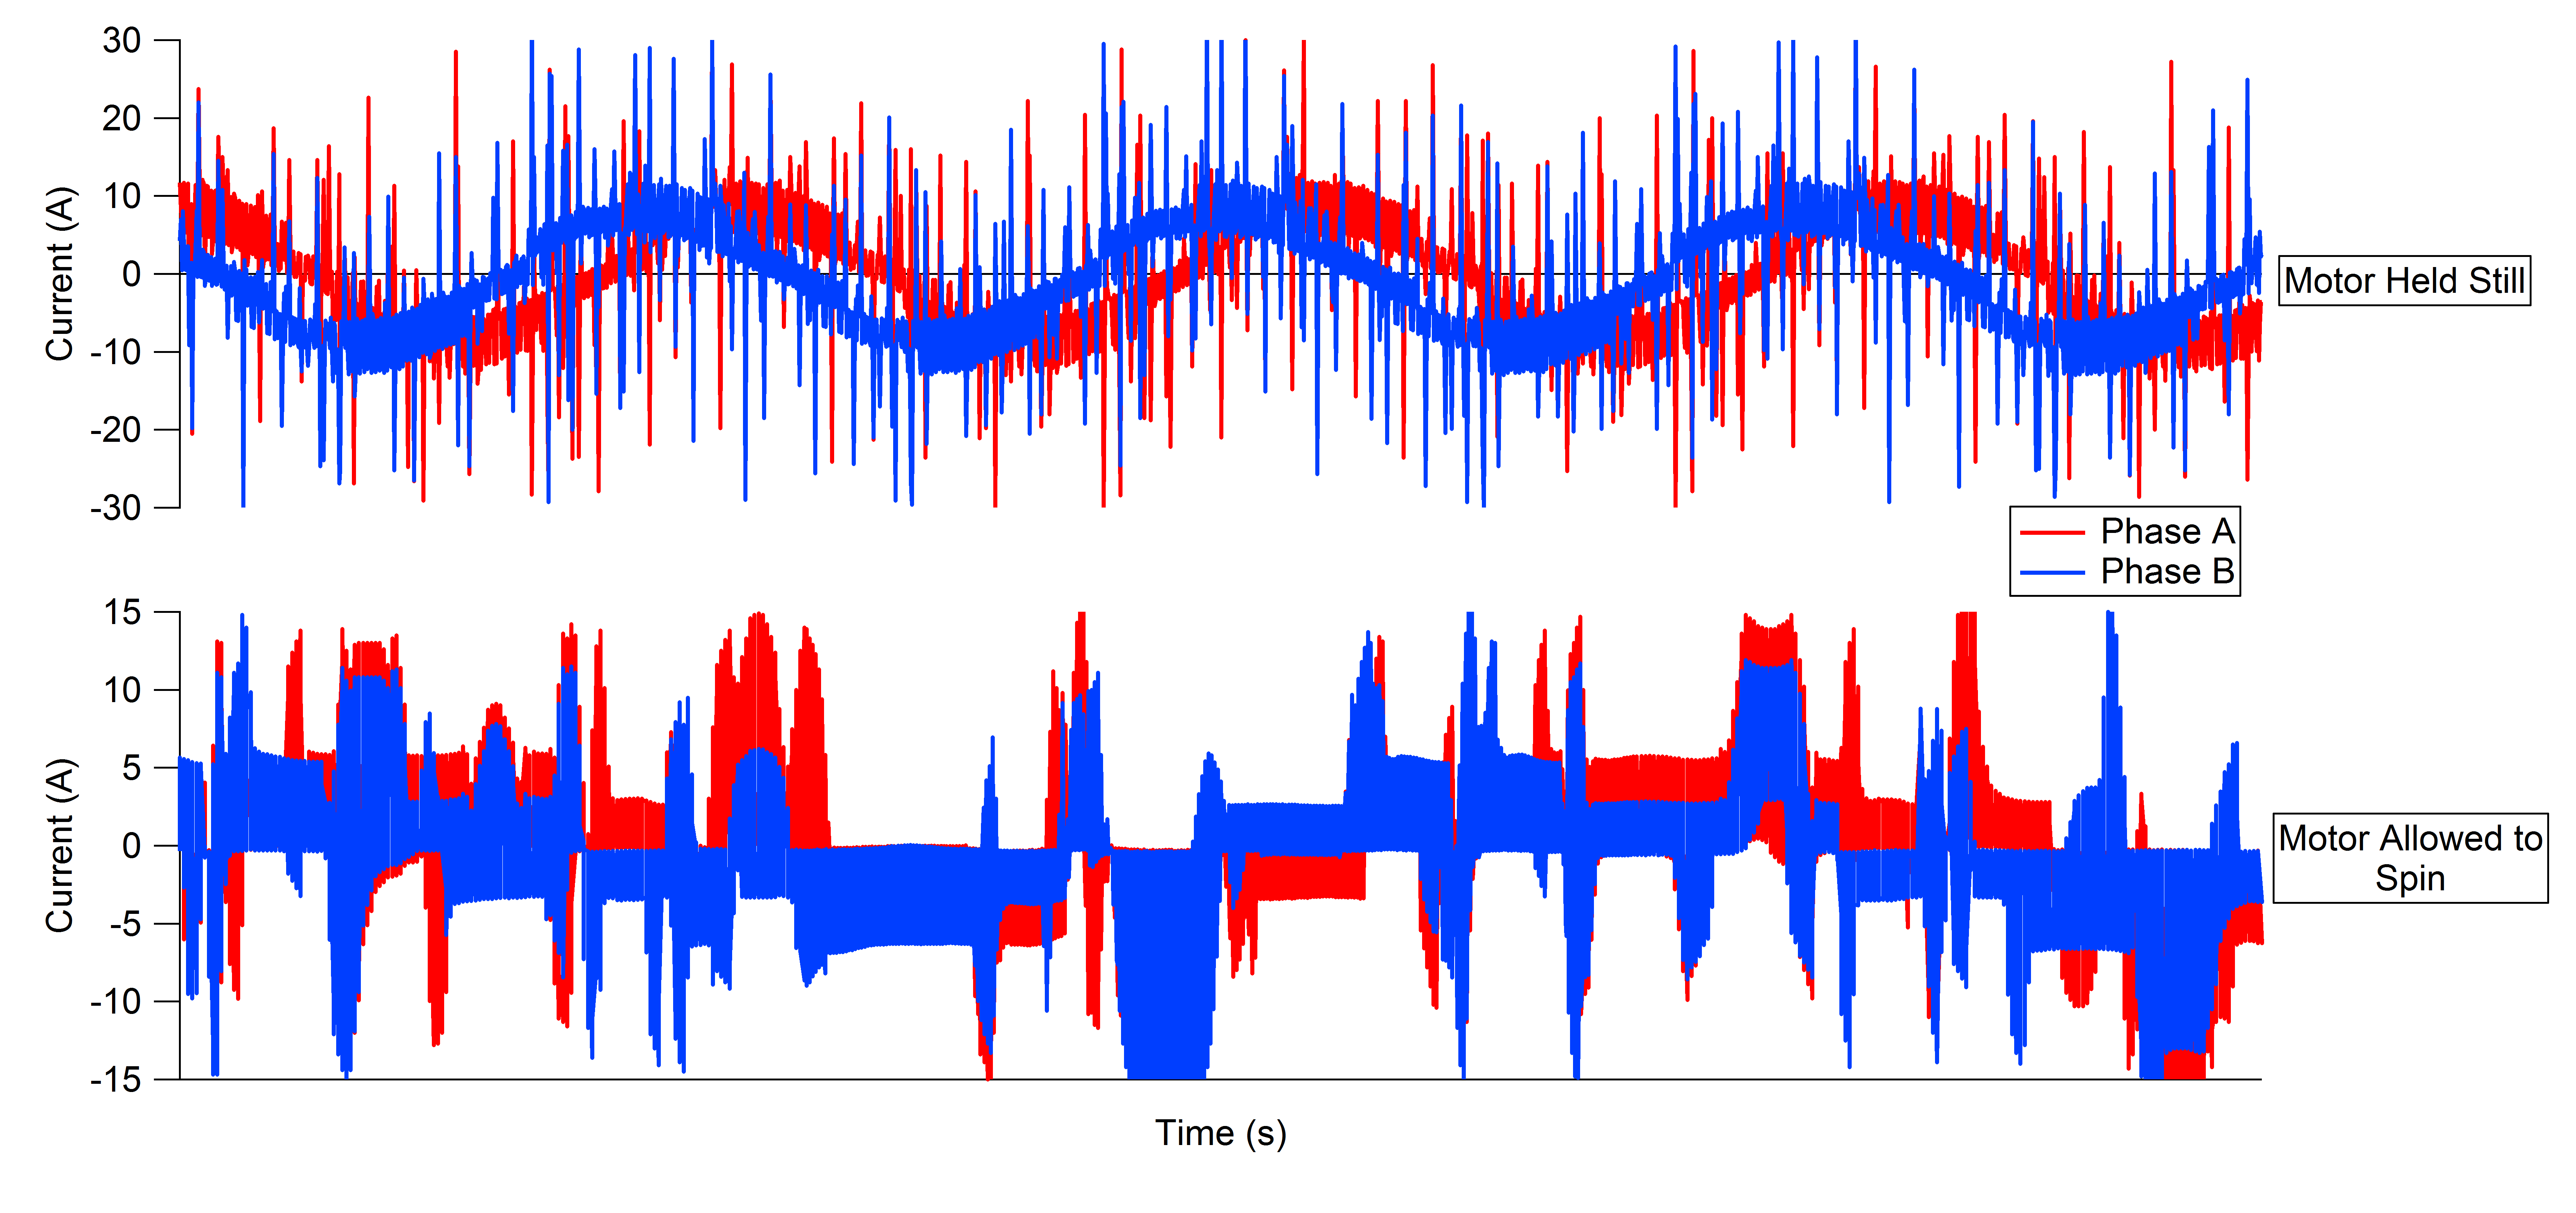
\includegraphics[scale=0.32]{Data/SPWM_Currentpng.png}
\label{SPWM_Currentpng}
\end{figure}

\begin{figure}[H]
\centering
\caption{TPWM Current Waveform}
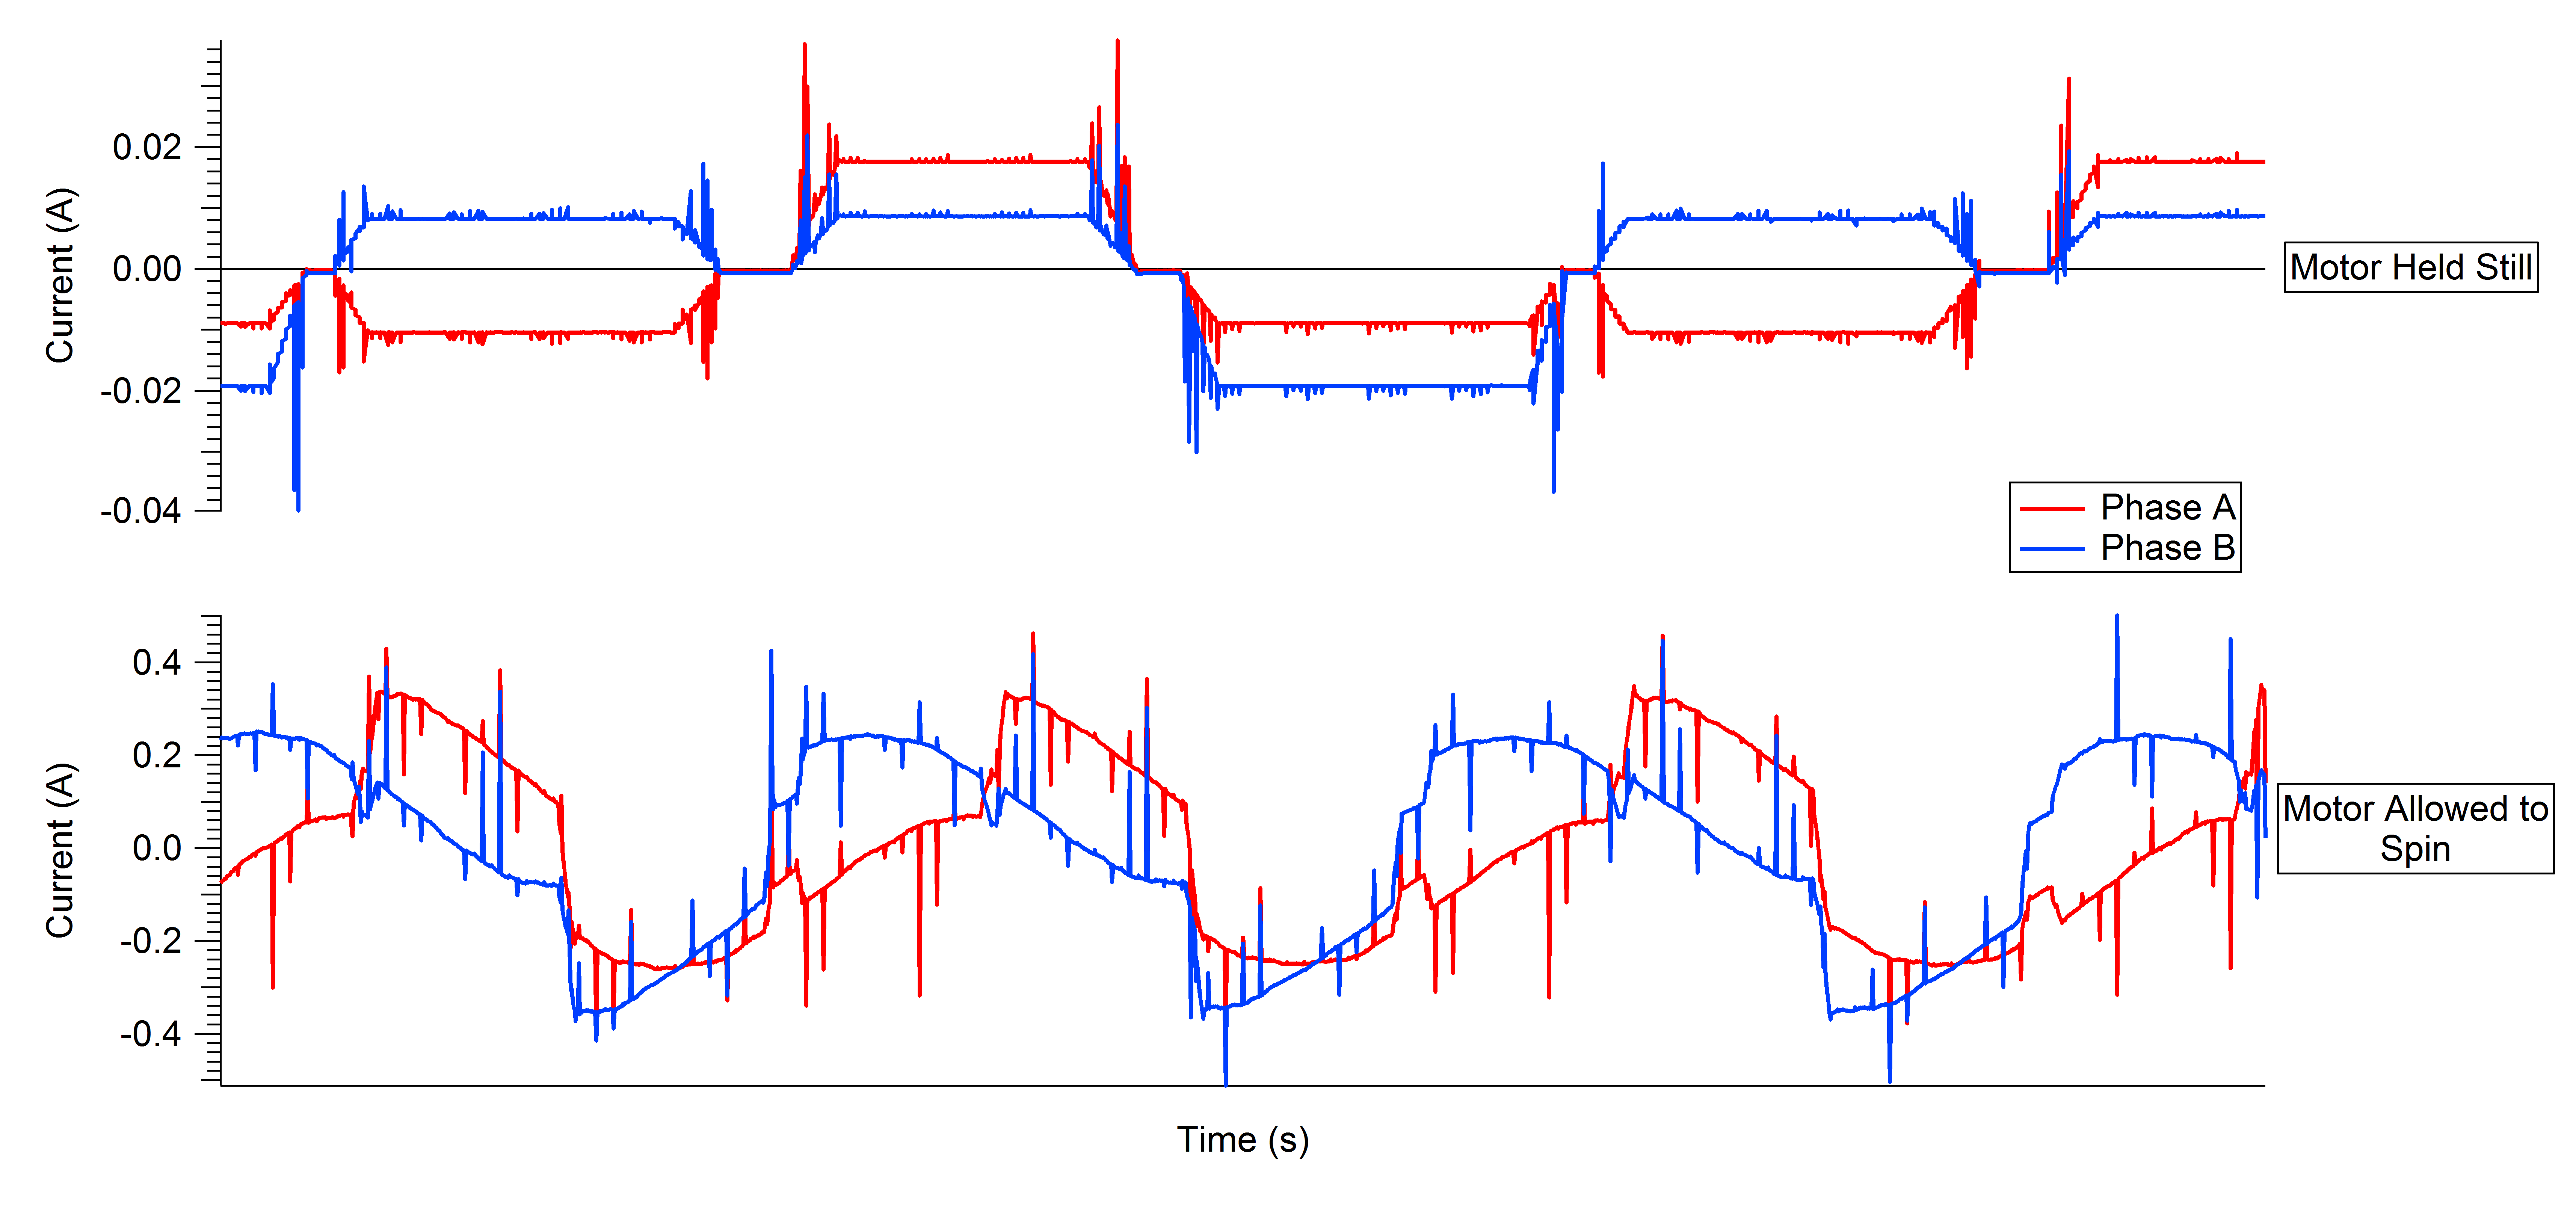
\includegraphics[scale=0.32]{Data/TPWM_Current.png}
\label{TPWM_Current}
\end{figure}

From the figures it is clear that the spinning of the motor produces irregularities in measurement which arise from the presence of non-linear back-emf voltages and timings. In the case of the still variants, the motor current is shown to behave in complete compliance to expectations. It is also important to note that as expected the TPWM control method generated significantly more bumpy operation in contrast to the SPWM mode.
\pagebreak
\section{Prototype Specifications}%done

Following the examination of the circuit operation the generalized performance specifications were summarized and are presented in Table~\ref{RESULTS}.

\begin{table}[H]
\centering
\caption{Prototype Characteristic Summary}
\label{RESULTS}
\resizebox{1.2\textwidth}{!}{
\begin{tabular}{|c|c|c|c|c|}
\hline
\textbf{Circuit Section} & \textbf{Parameter} & \textbf{Theoretical/Desired Value} & \textbf{Measured Value} & \textbf{\% Error} \\ \hline
Wien Bridge & Stability & Stable for all frequencies & Stable for $f<95Hz$ & N/A \\ \hline
Wien Bridge & $A_{f_{coefficient}}$ & $33.86Hz/k\Omega$ & $66.91\pm2.31 Hz/k\Omega$ & $49\%$ \\ \hline
Wien Bridge & Amplitide & Constant for all frequencies & Decays in accordance with $A=-1.483(R_s)^{-1}$ & N/A \\ \hline
Triangle Gen & Frequency & $1532Hz$ & $1122Hz\pm 13Hz$ & $27\%$ \\ \hline
Triangle Gen & Amplitude & Varriable with $R_a$ & Varriable with $R_a$ with upper limit & N/A \\ \hline
Phase Gen & PhaseAB & $120^{\circ}$ & $120.61\pm 0.48^{\circ}$ & $0.5\%$ \\ \hline
Phase Gen & PhaseAC & $-120^{\circ}$ & $-130.86\pm 0.52^{\circ}$ & $7\%$ \\ \hline
SPWM Gen & Amplitude Control & Full Control With $R_a$ & Full Control With $R_a$ produces TPWM at low $R_a$ & N/A \\ \hline
TPWM Gen & Amplitude Control & Full Control With $R_a$ & Control With $R_a$ from 100\% to 30\% of Max Power & N/A \\ \hline
Motor & SPWM & Operates Smoothly & Operates Smoothly & N/A \\ \hline
Motor & TPWM & Operates Bumpy & Operates Bumpy & N/A \\ \hline
\end{tabular}
}
\end{table}

\section{Proof of Design Demonstration}%done

The final design demonstration is to be conducted by allowing audience members to physical control the motor parameters through easily accessible potentiometers (as seen in Figure \ref{POTS}) and directly observe their effect on the "EMAX" model motor when equipped with a light load. 

\begin{figure}[H]
\centering
\caption{Motor-Controller-Prototype Control Knobs}
\includegraphics[scale=0.09]{Circuits/POTS.jpg}
\label{POTS}
\end{figure}

An oscilloscope will also be used to display the various intermediate signal stages so that interested individuals can better grasp the analogue methods of generating Pulse Width Modulation control waveforms.
\pagebreak
\section{Conclusions}%done

In conclusion it was determined that the proposed electric motor PWM controller successfully allowed for the actuation of the provided three phase "EMAX Model 2213-935kV" BLDC motor and furthermore demonstrated the performance differences in operation between SPWM and TPWM techniques in accordance with theory. The following points outline the overall behavior of the physical circuit with respect to expectations.

\begin{enumerate}
    \item The Wien Bridge Oscillator was shown to provide adjustable frequencies with variation of $R_s$ and allowed for direct control of motor speed in both SPWM and TPWM modes of operation.
    \item The relative accuracy of the three phase generator was shown to be reasonably acceptable and provided the necessary offset needed to actuate the motor in the desired direction.
    \item Amplitude Control of both SPWM and TPWM modes of operation was successfully accomplished with variation of $R_a$ and allowed for direct current regulation of the motor.
    \item The H-Bridge when combined with the respective input pulses allowed for the switching of current direction in the motor's main coils, thus producing a rotational force.
    \item The SPWM motor response was shown to be significantly smoother then the TPWM response in accordance with the theory outlined in Section 3.
\end{enumerate}

It is recommended that additional analysis be conducted to quantify the differences between the SPWM and TPWM effects on the motor through the use of a tachometer. Such tests would also allow for calibration of the various controls and result in more formal controller specifications.
\pagebreak
\section{Collaboration and Participation}%done

In order to fulfil the course teamwork requirements as per the Canadian Engineering Accreditation Board directives the project was conducted as a joint effort between both authors. Table \ref{collaboration} illustrates a general overview of the division of duties between the two authors. Naturally not all aspects involved in the formalization of the project can be easily quantized or defined and as such said list serves only as a generalized overview of the division of work.

\begin{table}[H]
\centering
\caption{Author Contribution Summary}
\label{collaboration}
\begin{tabular}{|c|c|}
\hline
\textbf{Kurtus Schulz} & \textbf{Matthew Santos} \\ \hline
Brainstorming and Idea Selection & Initial Circuit Design \\ \hline
Research into Control and Design & LTspice Simulations \\ \hline
Part Selection and Associated Logistics & \multicolumn{1}{l|}{Circuit Implementation and Initial Testing} \\ \hline
Formalization of Project Proposal & Circuit Refinements and Modifications \\ \hline
Prototype Testing and Evaluation & Detailed Analysis of Circuit Operation \\ \hline
Reviewing and Editing of Final Report & Formalization of Final Report \\ \hline
\multicolumn{2}{|c|}{Final Demo Presentation} \\ \hline
\end{tabular}
\end{table}

%References Section (%done)
\pagebreak
\addcontentsline{toc}{section}{References}
\nocite{*}
\bibliographystyle{amsplain}
\bibliography{bibliography.bib}

\pagebreak

%Appendix Section

\begin{appendices}%done
\pagebreak

\section{Circuit Schematics} %fix some annotations

\subsection{Overall Circuit Schematic Diagram}%done
\begin{figure}[H]
\centering
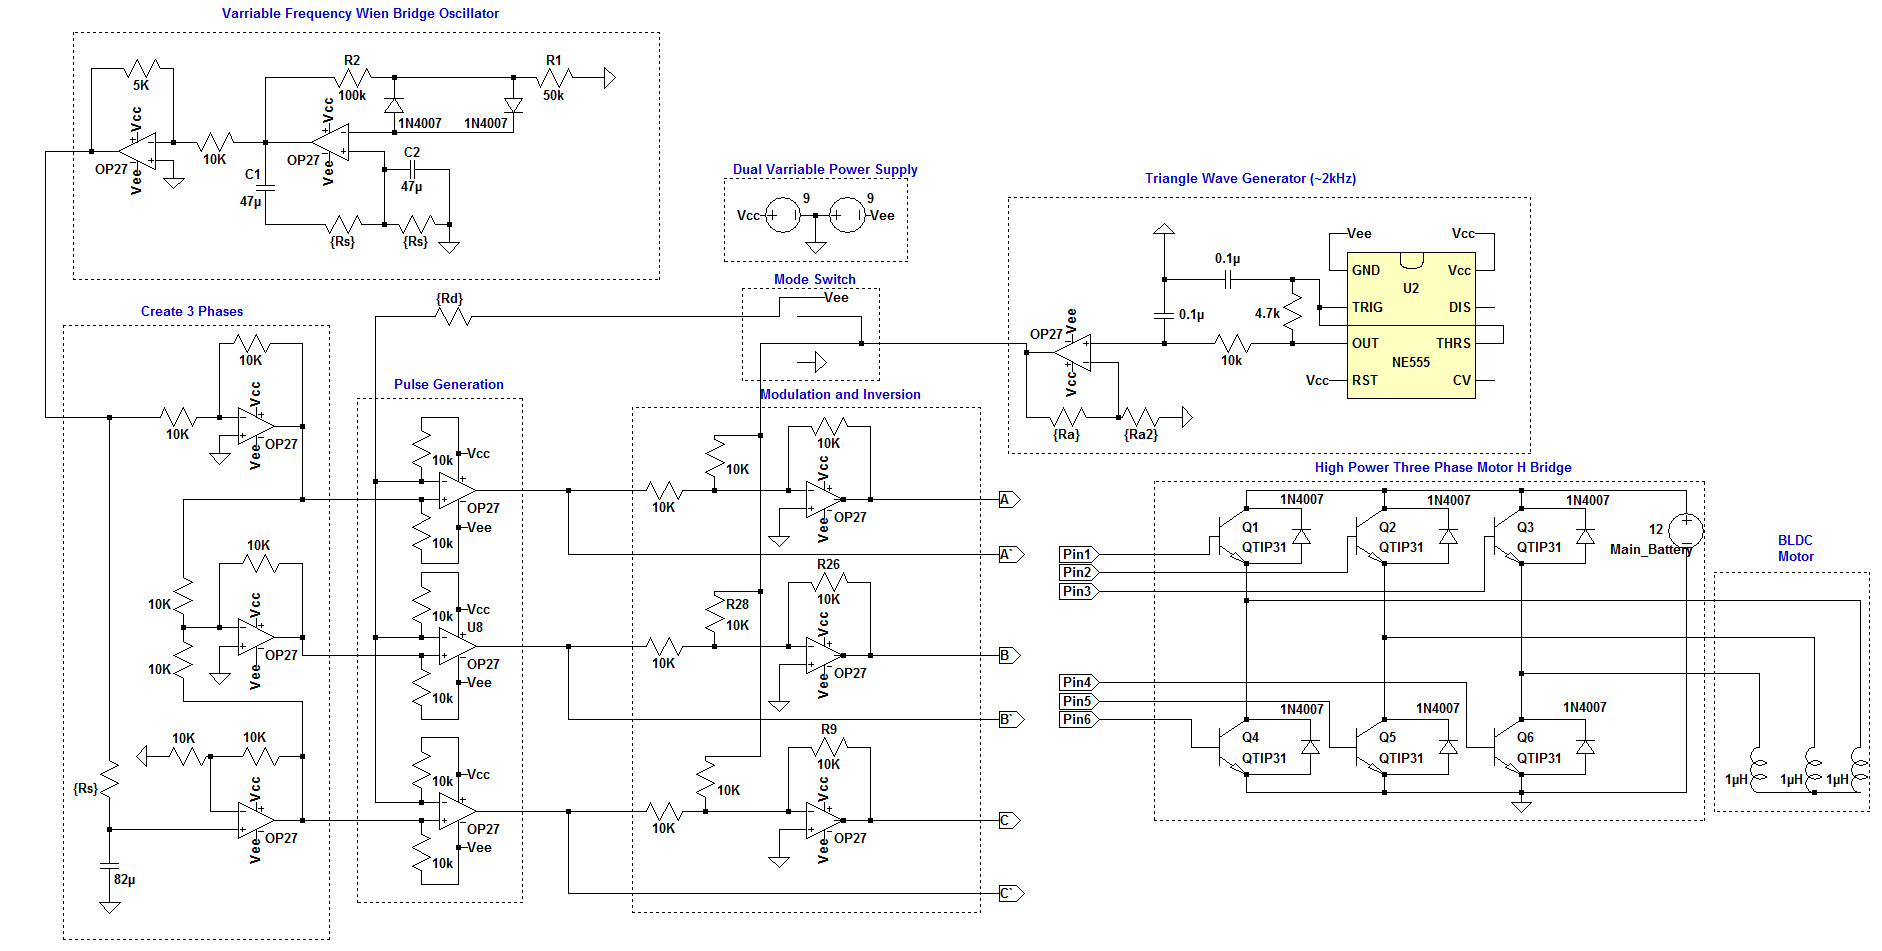
\includegraphics[scale=0.39,angle=90,origin=c]{Circuits/Overall_Design.png}
\label{Overall_Design}
\end{figure}
\subsection{Wien Bridge Oscillator Circuit}%done
\begin{figure}[H]
\centering
\includegraphics[scale=0.52,angle=90,origin=c]{Circuits/WBOCircuit.png}
\label{Overall_Design_V1}
\end{figure}
\subsection{Triangle Wave Generator Circuit}%done
\begin{figure}[H]
\centering
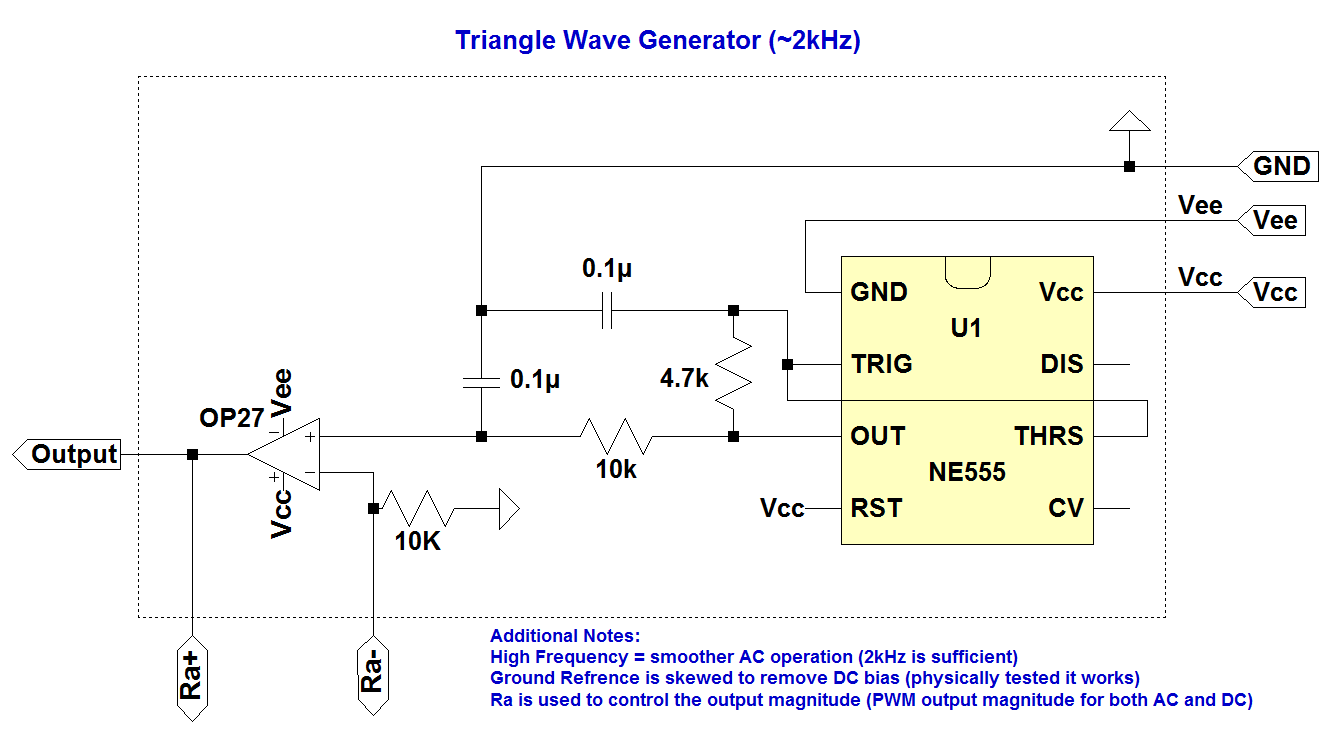
\includegraphics[scale=0.52,angle=90,origin=c]{Circuits/Triangle_Wave_Generator.png}
\label{Overall_Design_V1}
\end{figure}
\subsection{Phase Generation Circuit}%done
\begin{figure}[H]
\centering
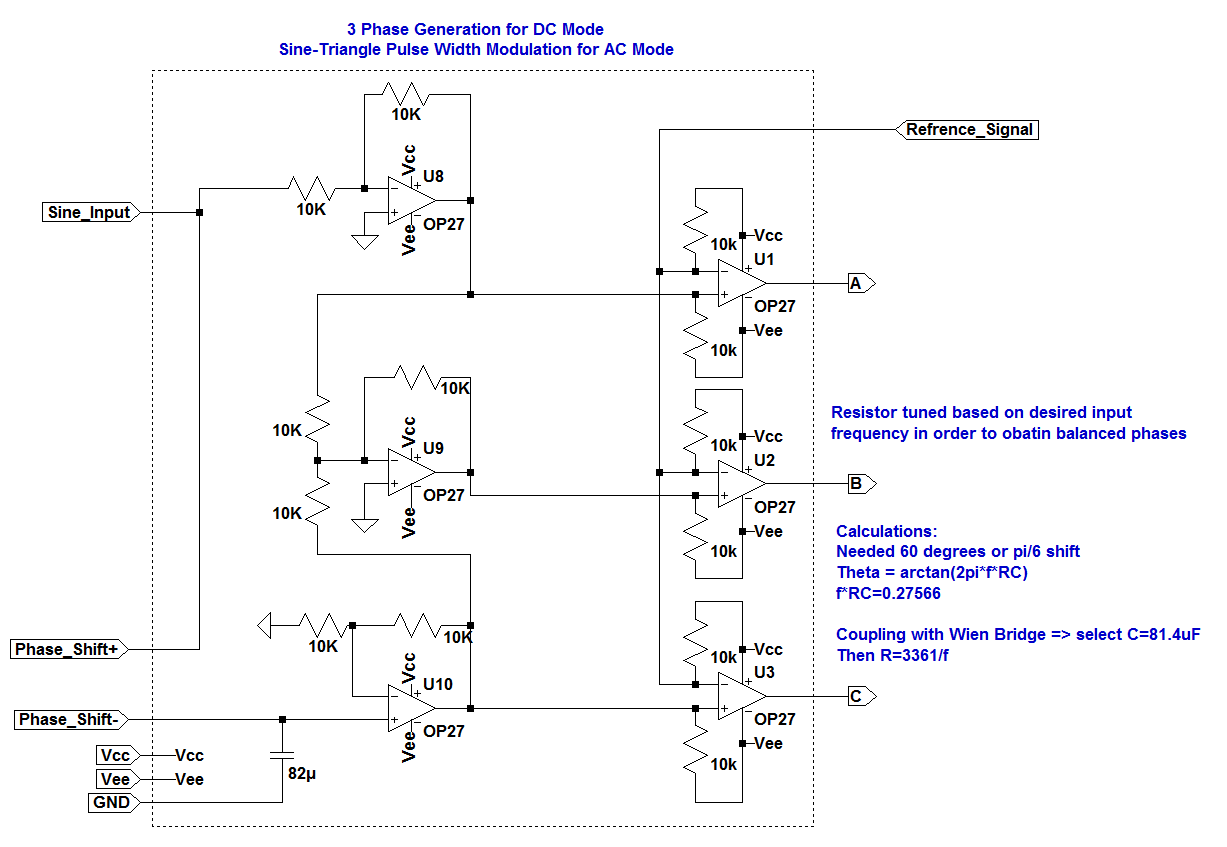
\includegraphics[scale=0.52,origin=c]{Circuits/Phase_Generation.png}
\label{Overall_Design_V1}
\end{figure}
\subsection{Modulation and Inversion Circuit}%done
\begin{figure}[H]
\centering
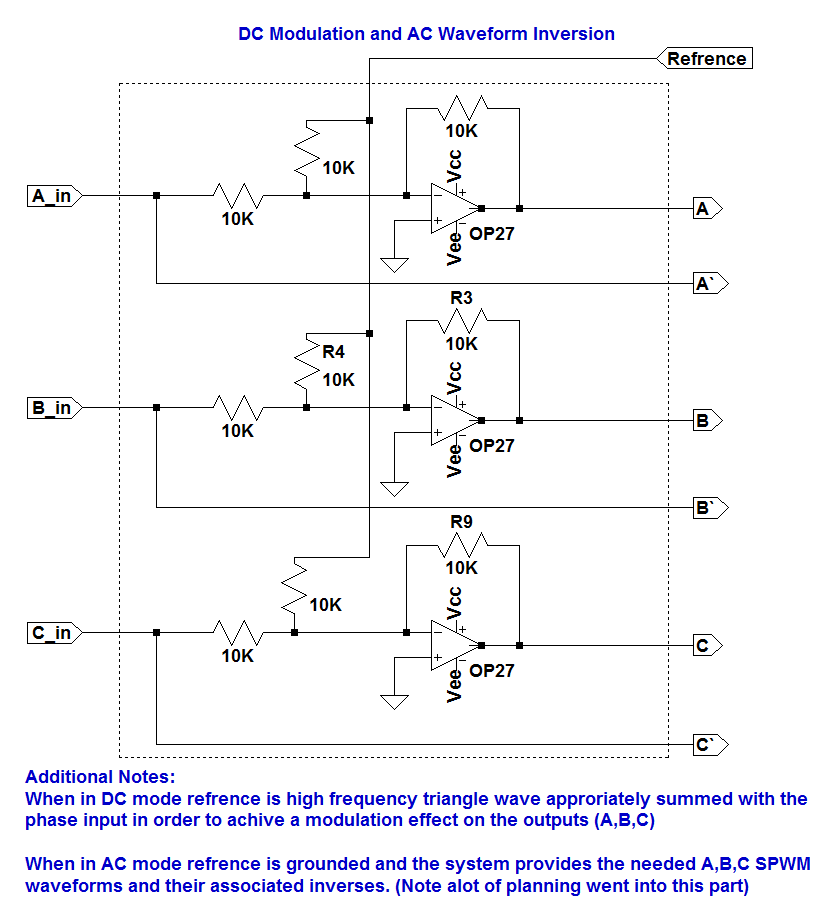
\includegraphics[scale=0.52,origin=c]{Circuits/Modulation_and_Inversion.png}
\label{Overall_Design_V1}
\end{figure}
\subsection{H-Bridge Three Phase Driver Circuit}%done
\begin{figure}[H]
\centering
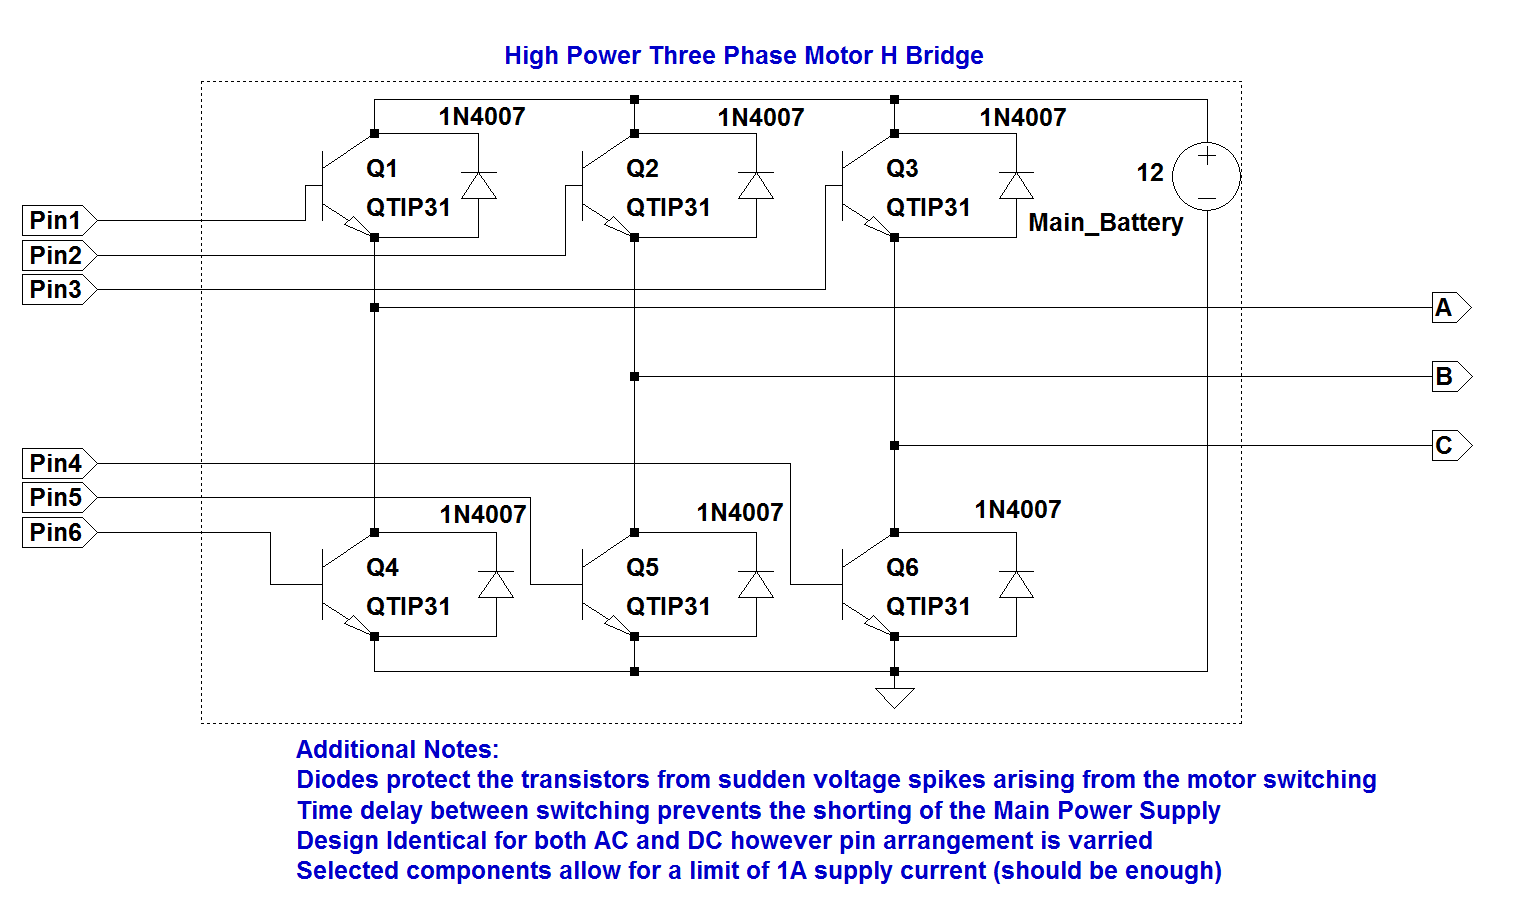
\includegraphics[scale=0.45,angle=90,origin=c]{Circuits/H_bridge.png}
\label{Overall_Design_V1}
\end{figure}

\pagebreak
\section{Simulation Results}%done

\subsection{Wien Bridge Oscillator Simulated Output}%done
\begin{figure}[H]
\centering
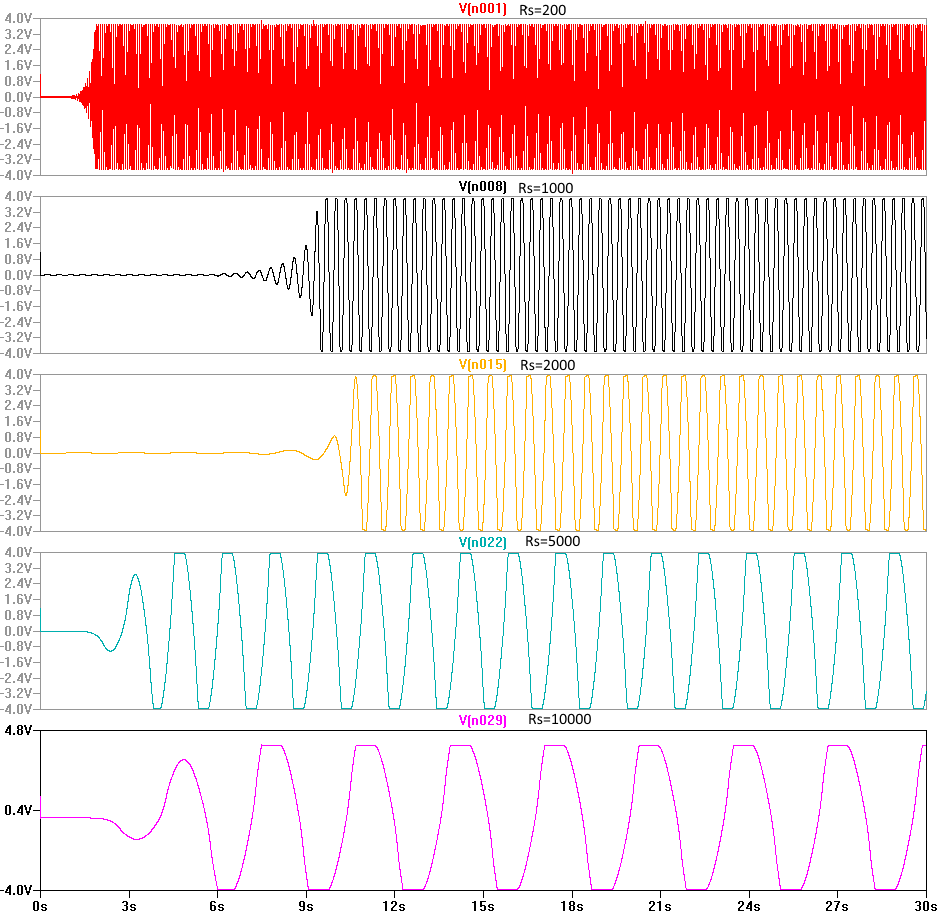
\includegraphics[scale=0.56,origin=c]{Data/Wein_Bridge_Output.png}
\label{Triangle_Gen_Output}
\end{figure}
Thus it is shown that the adjustment of $R_s$ correctly adjusts frequency output while maintaining overall magnitude. It is noted that the oscillations take time in order to reach saturation. Through the manipulation of Rs frequencies between 100Hz and 0.22Hz are theorized.

\subsection{Triangle Wave Generator Simulated Output}%done
\begin{figure}[H]
\centering
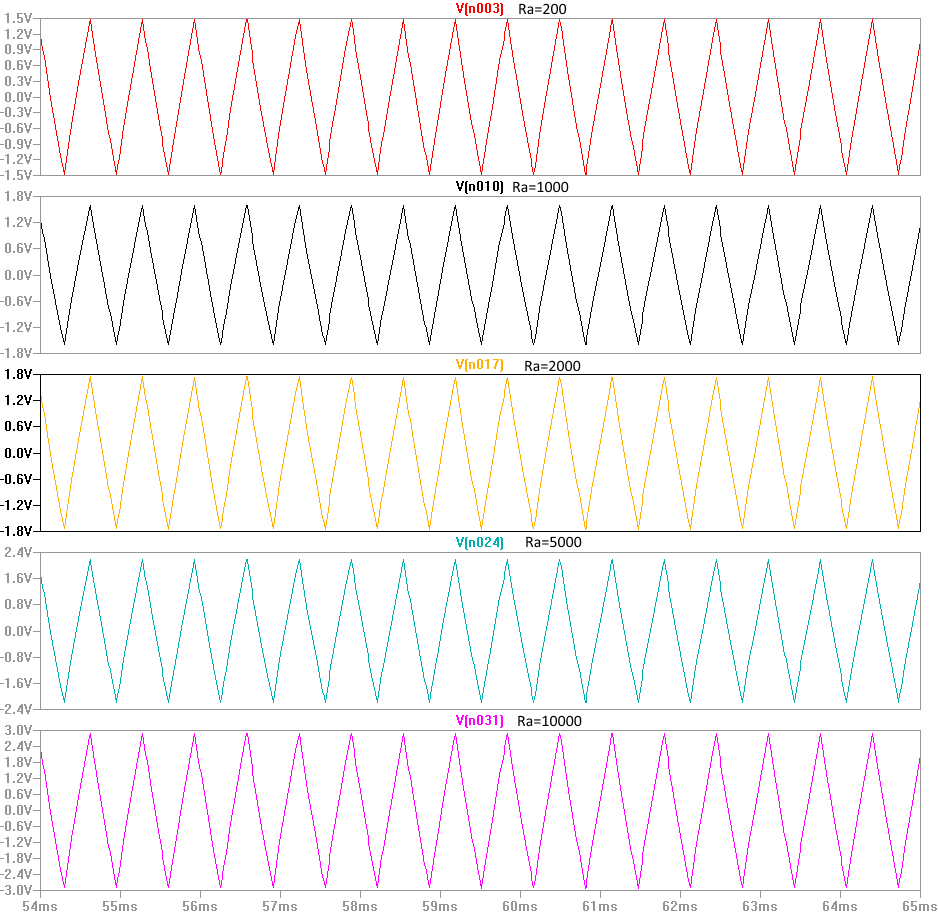
\includegraphics[scale=0.56,origin=c]{Data/Triangle_Wave_Output.png}
\label{Triangle_Gen_Output}
\end{figure}
As expected the frequency output of the generator is fixed at approximately 1500Hz which should be sufficient for both Modulation of the TPWM control signal and sine wave resolution during the SPWM configuration.The varying of the $R_a$ tuning resistor correctly adjusts the maximum output amplitude of the triangle wave from 1.5V to 3.0V as intended.

\subsection{Three Phase Sine Wave Generation}%done
\begin{figure}[H]
\centering
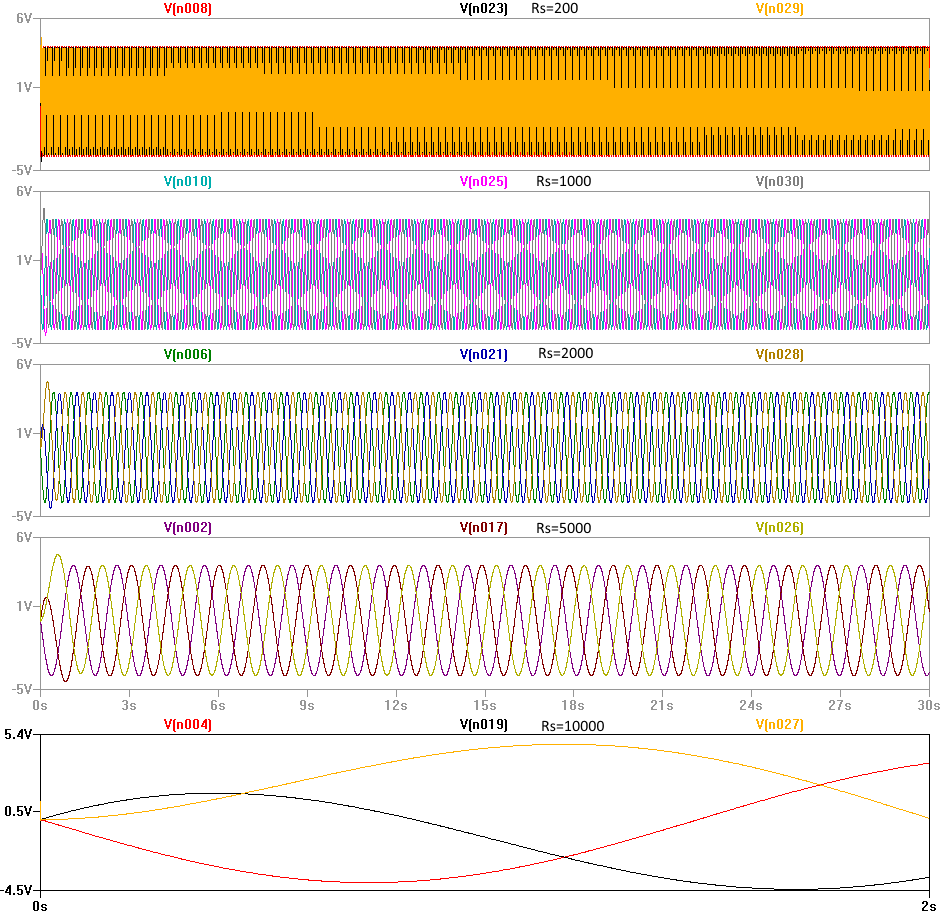
\includegraphics[scale=0.56,origin=c]{Data/3_Phase_Output.png}
\label{Triangle_Gen_Output}
\end{figure}

Through the solving of the associated system of equations the phase shifting circuit was tuned in conjunction with the Wien Bridge oscillator frequency set-point so that it will correctly produce the required 120 degree shifts at any frequency illustrated in the above simulation.

\subsection{Phase Generator Output (TPWM Configuration)}%done
\begin{figure}[H]
\centering
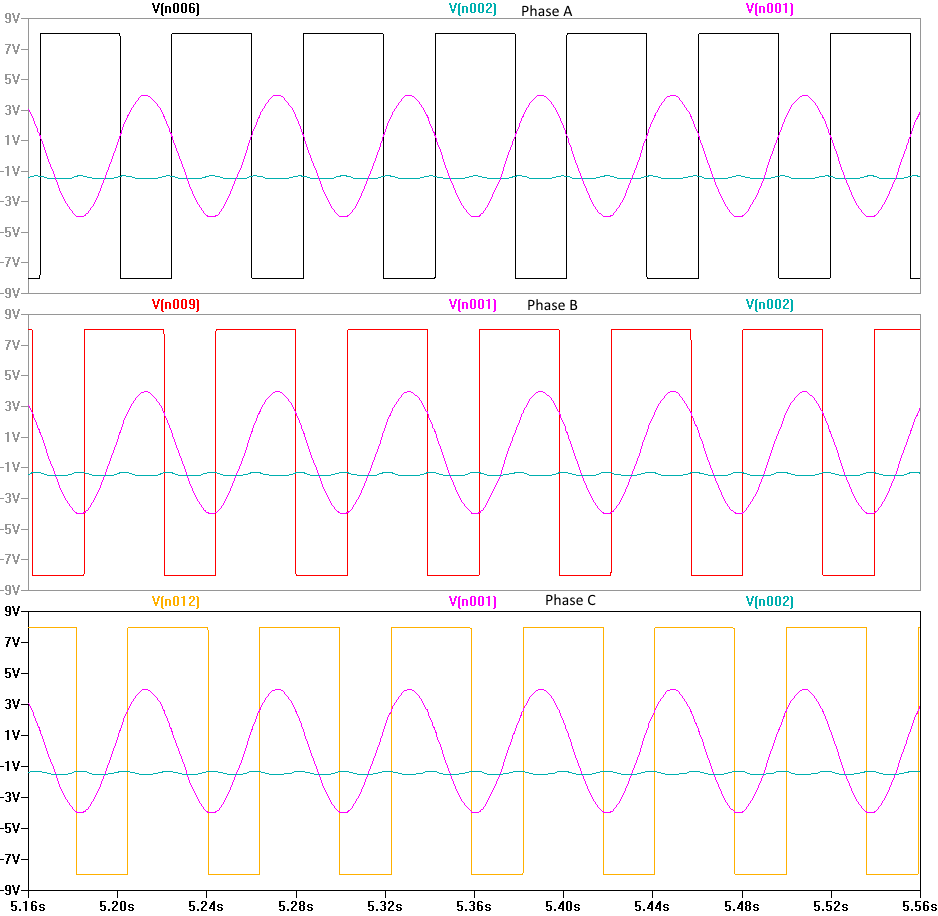
\includegraphics[scale=0.56,origin=c]{Data/DC_Refrenced_Phase_Generation_Output.png}
\label{Triangle_Gen_Output}
\end{figure}

The above simulation illustrates the production of the \emph{inverse} ON/OFF switching signals needed for commutation switching (about to be fed into an inverting summer). As illustrated these square wave signals are produced by comparing the 3 phase sine waves with a DC setpoint established through the tuning of Rd. Through alteration of this Rd resistance the spacing between switching events is varied as evident in the next figure.

\begin{figure}[H]
\centering
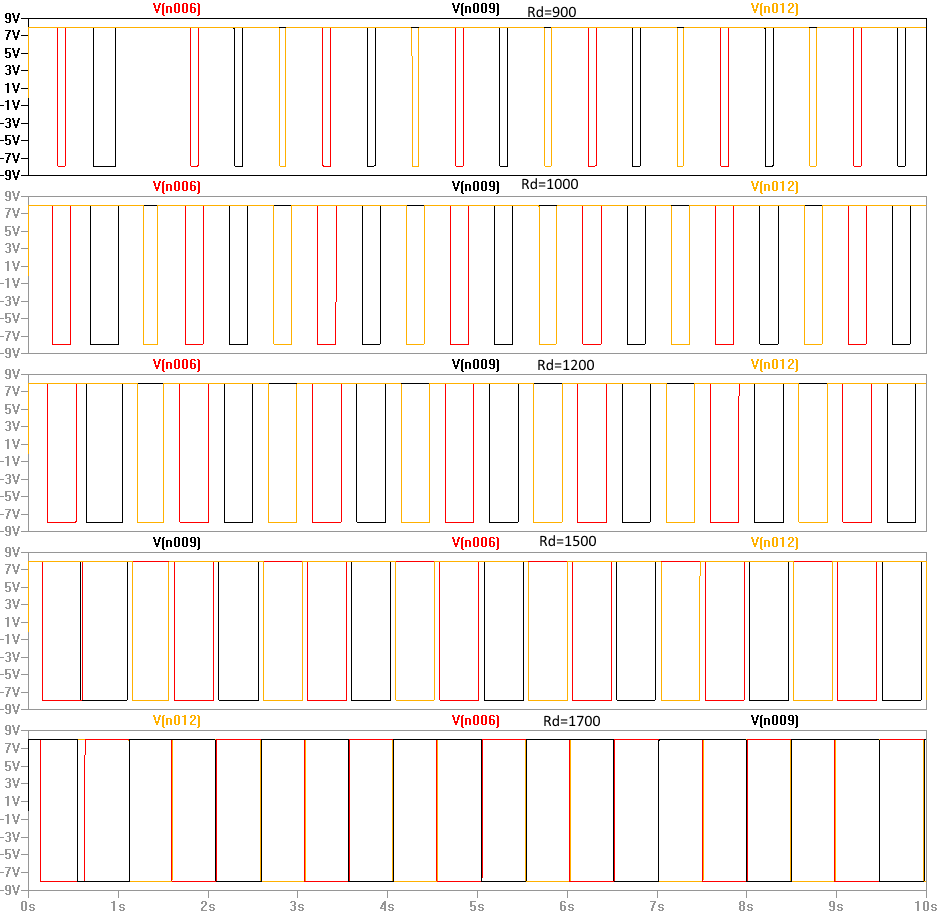
\includegraphics[scale=0.56,origin=c]{Data/DC_Phase_Gen_Rd_Effect.png}
\label{Triangle_Gen_Output}
\end{figure}

From the figure it is clear to see that an increase in $R_d$ produces shorter delay between actuation events. Care must be taken to always ensure a delay so as to prevent direct shorting of the H-Bridge driver. While not a variable of primary importance control of this delay allows for a smoothing like effect on motor control and also doubles as another form of modulation adjustment.

\subsection{Phase Generator Output (SPWM Configuration)}%done
\begin{figure}[H]
\centering
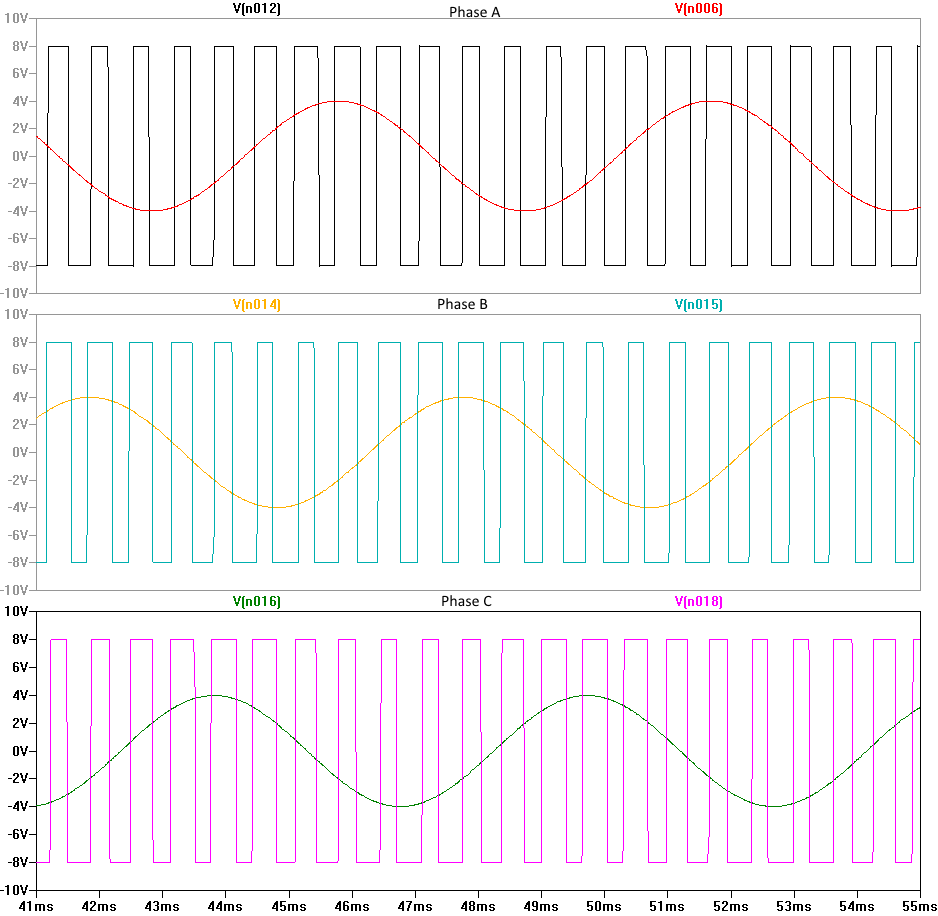
\includegraphics[scale=0.56,origin=c]{Data/AC_Phase_Gen_Output.png}
\label{Triangle_Gen_Output}
\end{figure}

Through the toggling of a switch the triangular waveform is set to connect to the reference terminal of the Phase Generator Circuit and its previous connection is then grounded. The 3 phase sine wave is directly compared with a high frequency triangle wave which is used to directly approximate the sine wave in the form of Sinewave Pulse Width Modulation (SPWM). The results are illustrated above.  These three signals can be used to directly drive the H-Bridge Circuit.

\subsection{Modulation and Inversion Output (TPWM Configuration)}%done
\begin{figure}[H]
\centering
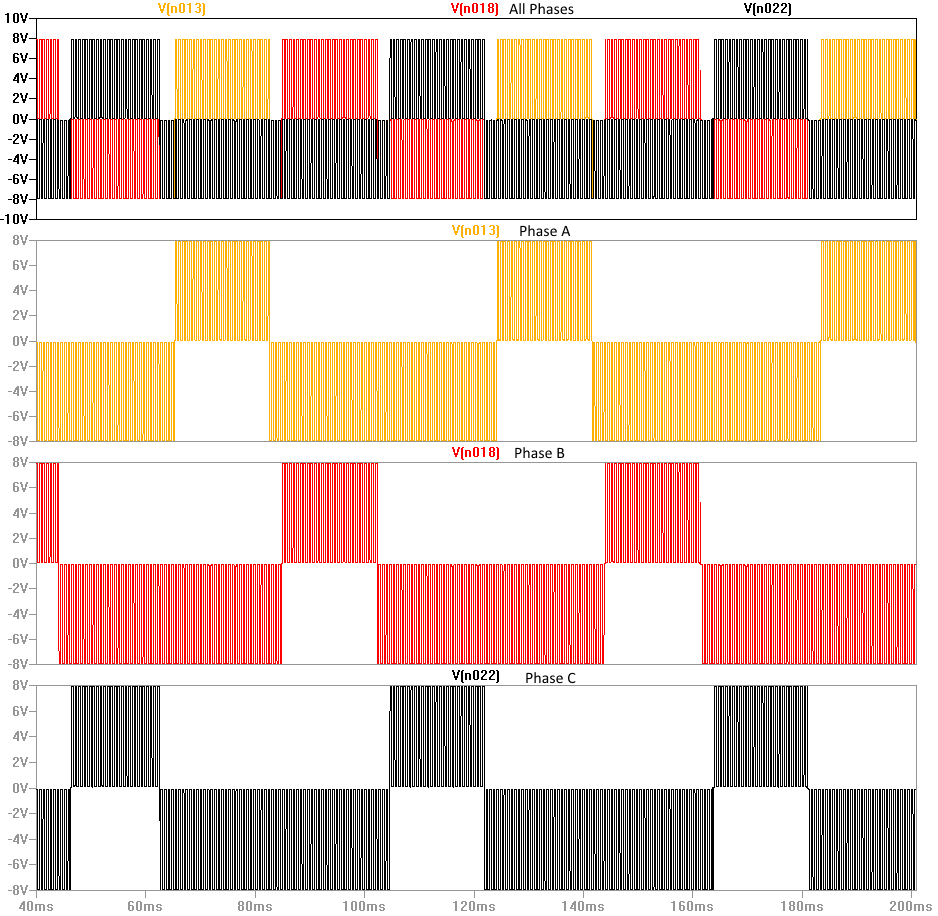
\includegraphics[scale=0.56,origin=c]{Data/Modulation_Inversion_DC_Output_High_Modulation.png}
\label{Triangle_Gen_Output}
\end{figure}

In TPWM configuration this circuit acts as an inverting summer which superimposes the high frequency triangular waveform on top of the previously generated square wave pulse signals. This has a modulation effect and through the varying of Ra can be used to adjust the average strength of the signal entering the H-Bridge Driver as illustrated in the next figure.

\begin{figure}[H]
\centering
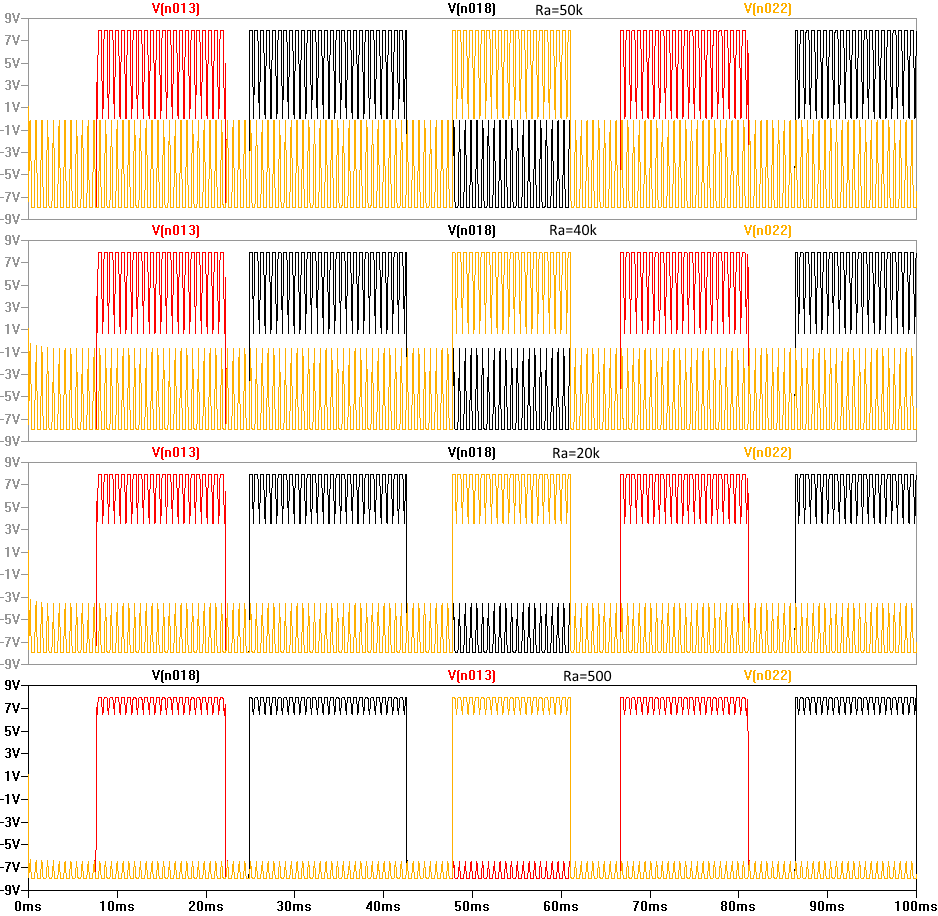
\includegraphics[scale=0.56,origin=c]{Data/Modulation_Inversion_DC_Output_Varied_Modulation.png}
\label{Triangle_Gen_Output}
\end{figure}

As illustrated above the altering of $R_a$ acts as a throttle on the output effectively adjusting its average amplitude through time based switching approximating the definition of pulse width modulation.

\subsection{Modulation and Inversion Output (SPWM Configuration)}%done

\begin{figure}[H]
\centering
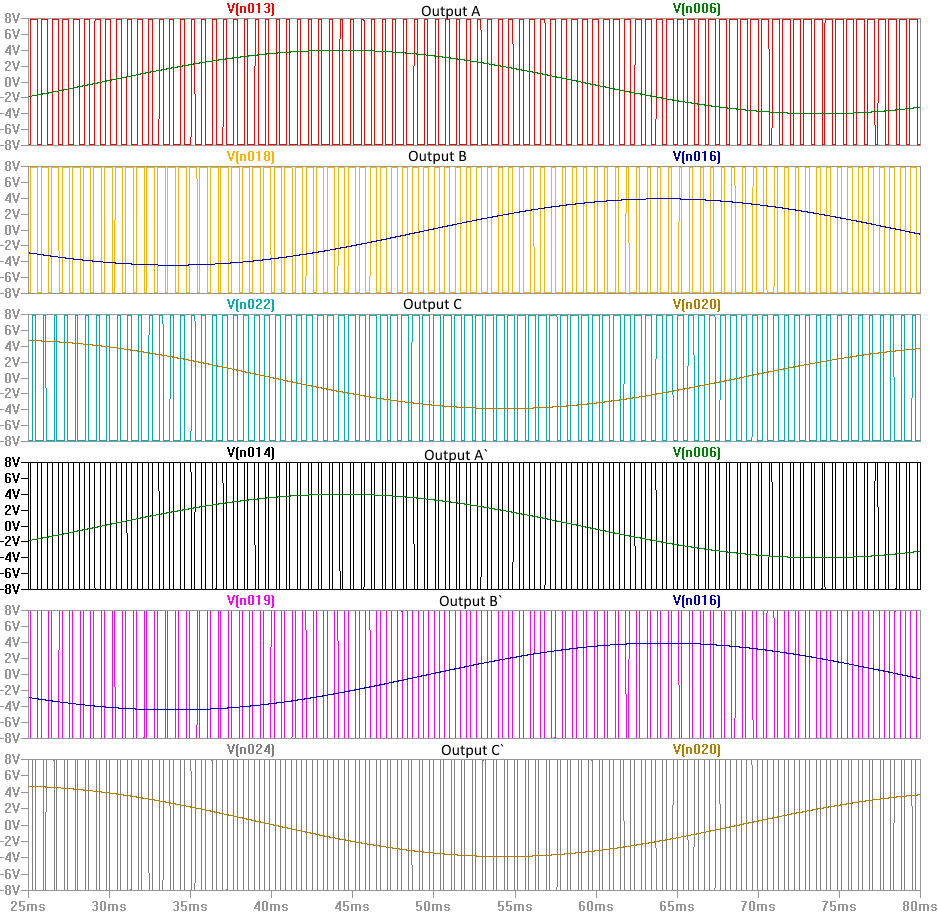
\includegraphics[scale=0.56,origin=c]{Data/AC_PWM_FINAL.png}
\label{Triangle_Gen_Output}
\end{figure}


In this configuration the circuit is simply an inverter and is used to extract the converse waveforms of the SPWM signals coming from the phase generator output. After inversion all the required signals for motor commutation are present and can be directly inserted into the H-bridge.

\subsection{Simulated Motor Current Waveforms}%done

In order to verify that the controller operates correctly the current waveforms in each of the windings were directly measured for TPWM configuration and the results are shown below.

\begin{figure}[H]
\centering
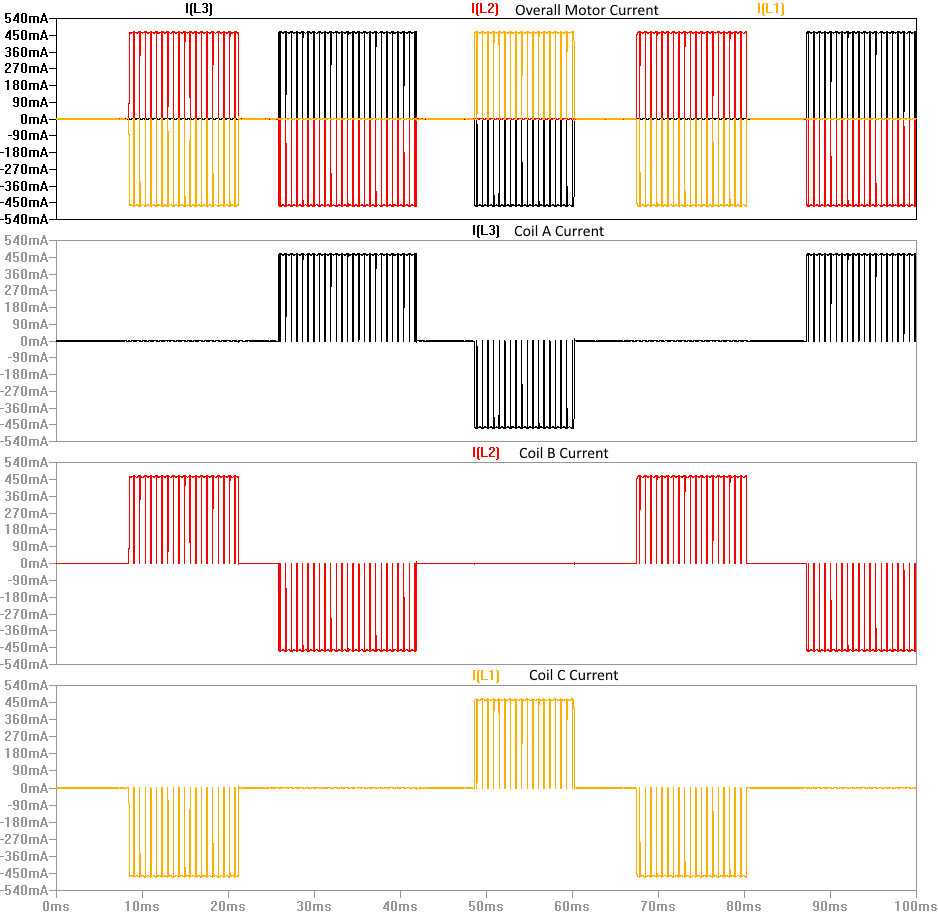
\includegraphics[scale=0.56,origin=c]{Data/Motor_OUTPUT_DC.png}
\label{Triangle_Gen_Output}
\end{figure}

From the figure it is clear that the motor is provided adequate current to actuate with a proper switching cycle including the needed delay to prevent the H-bridge from shorting.  

When examined in the SPWM configuration the motor exhibited the following current waveforms.

\begin{figure}[H]
\centering
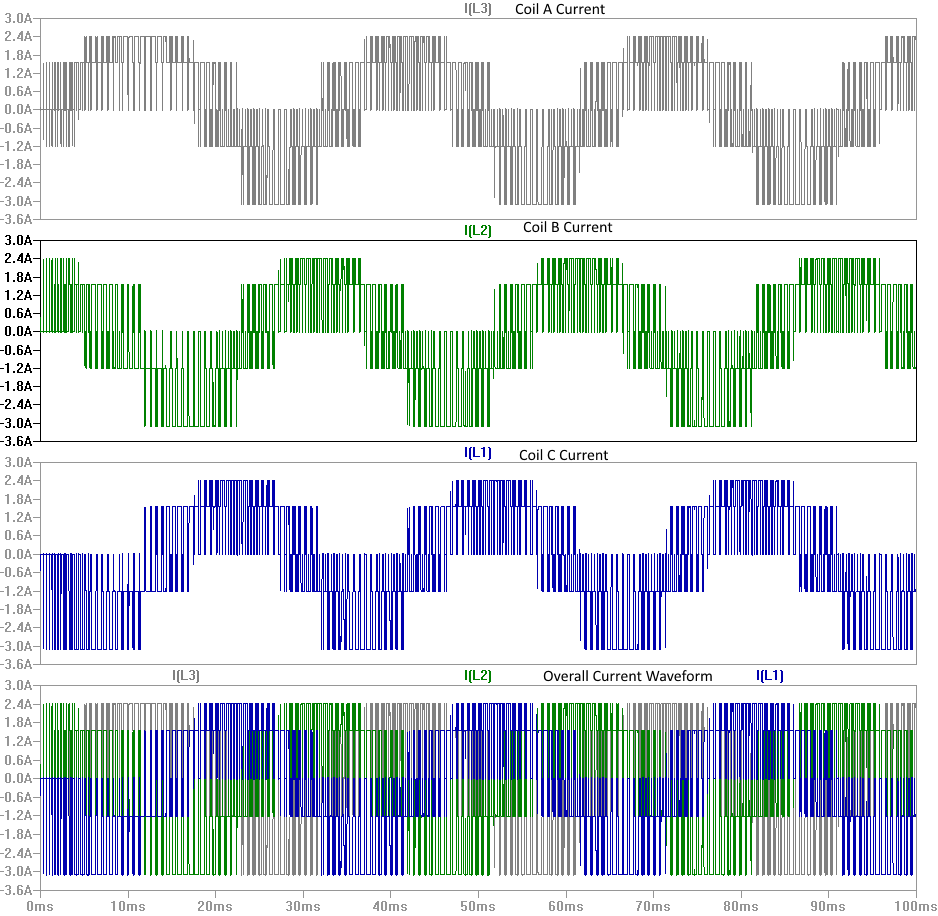
\includegraphics[scale=0.56,origin=c]{Data/Motor_OUTPUT_AC.png}
\label{Triangle_Gen_Output}
\end{figure}

From the figure it is clear that the motor is achieving commutation through the required waveform cycling which approximates a sinusoidal waveform.

\end{document}